%%%%%%%%%%%%%%%%%%%%%%%%%%%%%%%%%%%%%%%%%
% Masters/Doctoral Thesis 
% LaTeX Template
% Version 2.4 (22/11/16)
%
% This template has been downloaded from:
% http://www.LaTeXTemplates.com
%
% Version 2.x major modifications by:
% Vel (vel@latextemplates.com)
%
% This template is based on a template by:
% Steve Gunn (http://users.ecs.soton.ac.uk/srg/softwaretools/document/templates/)
% Sunil Patel (http://www.sunilpatel.co.uk/thesis-template/)
%
% Template license:
% CC BY-NC-SA 3.0 (http://creativecommons.org/licenses/by-nc-sa/3.0/)
%
%%%%%%%%%%%%%%%%%%%%%%%%%%%%%%%%%%%%%%%%%

%----------------------------------------------------------------------------------------
%	PACKAGES AND OTHER DOCUMENT CONFIGURATIONS
%----------------------------------------------------------------------------------------

\documentclass[
11pt, % The default document font size, options: 10pt, 11pt, 12pt
%oneside, % Two side (alternating margins) for binding by default, uncomment to switch to one side
catalan, % ngerman for German
singlespacing, % Single line spacing, alternatives: onehalfspacing or doublespacing
%draft, % Uncomment to enable draft mode (no pictures, no links, overfull hboxes indicated)
%nolistspacing, % If the document is onehalfspacing or doublespacing, uncomment this to set spacing in lists to single
%liststotoc, % Uncomment to add the list of figures/tables/etc to the table of contents
%toctotoc, % Uncomment to add the main table of contents to the table of contents
%parskip, % Uncomment to add space between paragraphs
%nohyperref, % Uncomment to not load the hyperref package
headsepline, % Uncomment to get a line under the header
%chapterinoneline, % Uncomment to place the chapter title next to the number on one line
%consistentlayout, % Uncomment to change the layout of the declaration, abstract and acknowledgements pages to match the default layout
]{MastersDoctoralThesis} % The class file specifying the document structure

\usepackage[utf8]{inputenc} % Required for inputting international characters
\usepackage[T1]{fontenc} % Output font encoding for international characters
\usepackage{eurosym}
\usepackage{footnote}
\usepackage{palatino} % Use the Palatino font by default
\usepackage{babel}
\usepackage[backend=bibtex,natbib=true]{biblatex} % Use the bibtex backend with the authoryear citation style (which resembles APA)
\usepackage{multirow}
\usepackage{float}

\addbibresource{example.bib} % The filename of the bibliography

\usepackage[autostyle=true]{csquotes} % Required to generate language-dependent quotes in the bibliography

%----------------------------------------------------------------------------------------
%	MARGIN SETTINGS
%----------------------------------------------------------------------------------------

\geometry{
	paper=a4paper, % Change to letterpaper for US letter
	inner=2.5cm, % Inner margin
	outer=3.8cm, % Outer margin
	bindingoffset=.5cm, % Binding offset
	top=1.5cm, % Top margin
	bottom=1.5cm, % Bottom margin
	%showframe, % Uncomment to show how the type block is set on the page
}

%----------------------------------------------------------------------------------------
%	THESIS INFORMATION
%----------------------------------------------------------------------------------------

\thesistitle{Wisebite} % Your thesis title, this is used in the title and abstract, print it elsewhere with \ttitle
\supervisor{Ernest Teniente} % Your supervisor's name, this is used in the title page, print it elsewhere with \supname
\examiner{} % Your examiner's name, this is not currently used anywhere in the template, print it elsewhere with \examname
\degree{Grau en Enginyeria Informàtica} % Your degree name, this is used in the title page and abstract, print it elsewhere with \degreename
\author{Albert Suàrez} % Your name, this is used in the title page and abstract, print it elsewhere with \authorname
\addresses{} % Your address, this is not currently used anywhere in the template, print it elsewhere with \addressname

\keywords{} % Keywords for your thesis, this is not currently used anywhere in the template, print it elsewhere with \keywordnames
\university{\href{http://www.upc.edu}{Universitat Politècnica de Catalunya}} % Your university's name and URL, this is used in the title page and abstract, print it elsewhere with \univname
\department{\href{https://www.essi.upc.edu/}{Departament d'Enginyeria de Serveis i Sistemes d'Informació}} % Your department's name and URL, this is used in the title page and abstract, print it elsewhere with \deptname
\group{\href{https://www.essi.upc.edu/}{ESSI}} % Your research group's name and URL, this is used in the title page, print it elsewhere with \groupname
\faculty{\href{http://www.fib.upc.edu}{Facultat d'Informàtica de Barcelona}} % Your faculty's name and URL, this is used in the title page and abstract, print it elsewhere with \facname

\AtBeginDocument{
\hypersetup{pdftitle=\ttitle} % Set the PDF's title to your title
\hypersetup{pdfauthor=\authorname} % Set the PDF's author to your name
\hypersetup{pdfkeywords=\keywordnames} % Set the PDF's keywords to your keywords
\hypersetup{linkcolor=black}
}

\newcolumntype{L}{>{\centering}m{0.75cm}}
\newcolumntype{M}{m{9cm}}
\newcolumntype{T}{m{12cm}}

\newcommand\tab[1][0.75cm]{\hspace*{#1}}

\begin{document}

\frontmatter % Use roman page numbering style (i, ii, iii, iv...) for the pre-content pages

\pagestyle{plain} % Default to the plain heading style until the thesis style is called for the body content

%----------------------------------------------------------------------------------------
%	TITLE PAGE
%----------------------------------------------------------------------------------------

\begin{titlepage}
\begin{center}


\includegraphics[scale=0.25]{Figures/logo-upc.png} % University/department logo - uncomment to place it

\vspace*{.06\textheight}
{\scshape\LARGE \univname\par}\vspace{1.5cm} % University name
\textsc{\Large Treball Final de Grau}\\[0.5cm] % Thesis type

\HRule \\[0.4cm] % Horizontal line
{\huge \bfseries \ttitle\par}\vspace{0.4cm} % Thesis title
\HRule \\[1.5cm] % Horizontal line
 
\begin{minipage}[t]{0.4\textwidth}
\begin{flushleft} \large
\emph{Autor:}\\
\href{http://www.johnsmith.com}{\authorname} % Author name - remove the \href bracket to remove the link
\end{flushleft}
\end{minipage}
\begin{minipage}[t]{0.4\textwidth}
\begin{flushright} \large
\emph{Director:} \\
\href{http://www.jamessmith.com}{\supname} % Supervisor name - remove the \href bracket to remove the link  
\end{flushright}
\end{minipage}\\[3cm]
 
\vfill

\large \textit{Un treball final de grau corresponent\\ al \degreename}\\[0.3cm] % University requirement text
\textit{en el}\\[0.4cm]
\deptname\\[2cm] % Research group name and department name
 
\vfill

{\large \today}\\[4cm] % Date
 
\vfill
\end{center}
\end{titlepage}


%----------------------------------------------------------------------------------------
%	ABSTRACT PAGE
%----------------------------------------------------------------------------------------

\begin{abstract}
\addchaptertocentry{\abstractname} % Add the abstract to the table of contents
La tecnologia està evolucionant de forma exponencial en els últims anys. Tot i així, sembla que hi ha un seguit de sectors en la societat que no s'acaben d'adaptar a aquest canvi. Un d'aquests sectors és el la restauració. Ja poden existir sistemes d'Intel·ligència Artificial que et realitzen la comanda al supermercat de forma automàtica, però encara avui en dia es veuen establiments com bars i restaurants que encara realitzen les comandes a bolígraf i paper. La pregunta que ens realitzem és: per què està passant això? En aquest treball final de grau s'ha estudiat els motius i s'ha analitzat com podria ser la millor solució pel problema comentat.
\\\\
\textit{Wisebite}, la plataforma que gestiona de forma intel·ligent els establiments de restauració, té com a objectiu solucionar aquesta problemàtica. Així, no només modernitzaria el sector, sinó que també podria oferir millors resultats en qualitat de servei, eficiència i beneficis econòmics als establiments que decideixin implantar-la.
\end{abstract}

%----------------------------------------------------------------------------------------
%	THESIS CONTENT - CHAPTERS
%----------------------------------------------------------------------------------------

\tableofcontents % Prints the main table of contents

\mainmatter % Begin numeric (1,2,3...) page numbering

\pagestyle{thesis} % Return the page headers back to the "thesis" style

% Include the chapters of the thesis as separate files from the Chapters folder
% Uncomment the lines as you write the chapters

% Chapter 1

\chapter{Introducció} % Main chapter title

\label{Chapter1} % For referencing the chapter elsewhere, use \ref{Chapter1} 

Aquest projecte és un Treball Final de Grau en Enginyeria Informàtica a la Facultat d'Informàtica de Barcelona (\textit{Universitat Politècnica de Catalunya}). Un projecte amb la finalitat principal de convertir un establiment de restauració qualsevol en quelcom intel·ligent, podent gestionar de forma més eficient, còmode i professional les seves comandes, podent-les analitzar posteriorment i interactuant de forma més activa amb el client de l'establiment.

\section{Contextualització}

El món de la restauració va néixer molts segles enrere i amb el transcurs de la història ha anat evolucionant proporcionalment amb l'evolució del ser humà i els seus costums. Tot i així, el que és clar és que el concepte d'anar a prendre quelcom al bar durant algun moment del dia es segueix mantenint per molt temps que passi, almenys a Espanya.
\\\\
La tecnologia ha estat quelcom que sempre ha existit, però no amb tanta importància i impacte com té actualment. Des del naixement de l'\textit{smartphone} \cite{smartphone} el 1992 quan IBM va treure el primer pilot de telèfon mòbil amb funcionalitats de PDA incorporades, s'ha anat instaurant a les nostres vides de manera exponencial fins al punt on és pràcticament una part nostra, que sense ella no seria el mateix. D'aquest aspecte se li pot treure tant punts favorables com negatius. Entre els positius tenim sistemes similars als del projecte que estem tractant, el qual dóna infinitats d'avantatges respecte al sistema convencional. Avui en dia, en el context de la societat actual en què vivim, sistemes intel·ligents implantats en els establiments de restauració es veuen a comptagotes, i no pas perquè les plataformes existents siguin dolentes o precàries, sinó per un altre seguit de factors. Factors com pot ser l'impacte econòmic que implica la instauració d'un sistema d'aquestes característiques, la manca d'adaptabilitat al canvi o bé la complexitat d'alguns establiments.
\\\\
El fet és que des de principis de segle els costums humans canvien amb una rapidesa realment diferent de la de fa segles, tan ràpidament que el món de la restauració en conjunt no s'ha pogut adaptar.
El naixement de les noves tecnologies i el poder que tenen avui en dia a la societat es veu reflectit en bars i restaurants, on algun d'ells (i cada cop més) la utilitzen en el negoci.
Tot i així, en l'estudi d'aquest tòpic, apareix un seguit de qüestions gens menyspreables, les quals han de ser tractades.

\subsection{Factor econòmic}

Un dels principals problemes per als quals aquest sector no s'ha acabat d'adaptar és el cost de la implantació de la tecnologia en un establiment d'aquestes característiques. Cada restaurant o bar és únic en referència a la resta, per tant, cada un d'ells necessita un sistema adaptat a les seves necessitats, i això es fa pagar.
\\\\
El desenvolupament d'un sistema genèric és notablement més barat respecte un específic, ja que l'equip encarregat de construir pot vendre-ho posteriorment a més d'un client, així doncs pot ajustar més el preu. En canvi, si estem parlant d'un sistema totalment personalitzat i especialitzat per un establiment, llavors el cost puja considerablement, ja que han de cobrir els costos del disseny i la implementació del sistema.
\\\\
És aquí doncs on s'estableix un dels tres grans problemes que fa que sistemes d'aquestes característiques no es vegin avui en dia en els establiments de restauració. A més a més se li suma l'època de crisi econòmica viscuda que fa complicar el panorama. Només els establiments que aconsegueixen facturar grans quantitats es poden permetre sistemes com el que comentem.

\subsection{Adaptació al canvi}

En aquest sector ens podem trobar molts tipus d'usuaris. Perfils de gent que sempre busquen ser millors en el sector i fan el possible per estar actualitzats amb la tecnologia d'aquell moment. 
En canvi, existeixen nombrosos casos d'establiments on els responsables d'aquests no tenen facilitat per adaptar-se al canvi, és a dir, que se satisfan amb el procediment de negoci que sempre han tingut i sempre els ha funcionat, encara que sigui antiquat. Amb dificultats com aquestes no és fàcil instaurar un sistema d'aquestes característiques, ja que els usuaris que la utilitzen no s'adaptarien i, en conseqüència, tindria represàlies negatives.
\\\\
La implantació de tot sistema en una corporació o empresa, ja sigui enfocat en el món de la restauració o bé en un altre sector, no només recau en la compra de material \textit{hardware} i \textit{software}, sinó que també recau en la implicació dels treballadors que hauran d'interactuar amb aquest nou sistema. Per tant, és obligació dels responsables de tot establiment que vulgui implantar un sistema d'aquestes característiques motivar a l'equip de treballadors en aquest aspecte. La plataforma a implantar ja pot ser molt bona, però si no hi ha voluntat de l'equip en utilitzar-la correctament, molt probablement el procés acabarà en fallida. 

\newpage
\subsection{Complexitat}

Tots els establiments d'aquest sector funcionen de maneres molt diferents acord a les seves característiques i funcionalitats. Alguns d'ells disposen de sistemes molt complexos i complicats en comparació de la competència, cosa que aporta dificultat en la implantació d'un sistema d'aquest tipus. I en contrapartida, implantar una plataforma d'aquestes característiques en un establiment molt simple com pot arribar a ser un bar de poble tampoc acaba de ser del tot útil.
\\\\
En conseqüència, podem tenir dues situacions que impedeixen el \textit{boom} d'aquests sistemes en el món de restauració. Per una banda, restaurants molt complexos que incapaciten crear un sistema que ho controli tot de forma fàcil. I per altra banda, bars molt simples o senzills que mai s'arribaran a plantejar sistemes d'aquestes característiques.

%----------------------------------------------------------------------------------------

\section{Motivació}

Durant el quadrimestre anterior a l'inici del Treball Final de Grau vaig estar rumiant profundament cap a on volia encaminar el projecte. Tenia disponible la capacitat de realitzar-ho en l'empresa en la qual estava treballant, i actualment segueixo. Tot i així, donades unes circumstàncies que es comentarà a continuació, vaig decidir encaminar-me a realitzar el projecte de \textit{Wisebite}.
\\\\
En el meu context familiar i d'amistats he tingut sempre molt present la cultura de la gastronomia, com bé caracteritza el nostre país. Tot i així, amb els anys he anat coneixent persones que es dediquen professionalment al món de la restauració, sigui cambrers, cuiners o administradors d'establiments del sector. En anar amb aquest tipus de persones a prendre quelcom o a menjar un àpat, em feien veure diferent l'establiment de com ho feia abans. Molts cops ens centràvem més en com era el servei i com estava muntat internament la cadena de producció dins l'establiment que pas gaudir de l'àpat que ens estaven servint.
\\\\
En conseqüència, arran d'això i dels coneixements tècnics que he anat adquirint durant el grau aquests quatre anys, vaig estar pensant com es podria aplicar la tecnologia en establiments d'aquest tipus per tal de millorar la seva eficiència i poder oferir un millor producte als clients.
\\\\
Per dissenyar i construir una idea més autèntica vaig estar parlant amb aquest grup de persones, que s'ha comentat anteriorment, i se'ls va preguntar com funcionaven els seus establiments i que realitzarien per poder millorar-los al que correspon a la gestió del bar o restaurant. Una gran majoria d'aquests em va comentar que van implantar un sistema de gestió de comandes a través d'un mòbil o tauleta, però que els havia costat molt temps acabar-ho implantant donat al cost que comportava. I no només això, sinó que els hi va costar bastant adaptar-se a causa de la poca usabilitat que tenia el sistema que utilitzaven.
\\\\
\newpage
Així doncs, vist quin era l'estat actual, vaig decidir-me a realitzar un estudi de mercat analitzant quines aplicacions i plataformes existien en aquell moment (apartat que comentarem posteriorment) i em vaig adonar que hi havia molta feina per fer. Les aplicacions que aplicaven la filosofia de \textit{Wisebite} estaven bastant obsoletes i no disposaven d'una interfície d'usuari que tendia a la usabilitat, fet que dificultava l'adaptabilitat al canvi dels usuaris.
\\\\
En conclusió, després d'estudiar bé la proposta vaig parlar l'\textit{Ernest Teniente} i va acceptar ser el meu director d'aquest projecte i Treball Final de Grau.
% Chapter Template

\chapter{Estat de l'art} % Main chapter title

\label{Chapter2} % Change X to a consecutive number; for referencing this chapter elsewhere, use \ref{ChapterX}

Per conèixer millor el potencial d'aquest mercat i saber les alternatives per a una major profunditat en el coneixement del sector, s'ha de realitzar un estudi del mercat existent per a comprovar la presència d'aplicacions que són similars, sigui per objectiu o per mercat, a \textit{Wisebite}. A continuació apareixen algunes de les aplicacions que s'han pogut trobar.
\\\\
El fet d'analitzar cadascuna d'elles et permet veure quines funcionalitats pots oferir al client perquè directament no existeix cap eina que les faciliti o bé per millorar les existents. S'ha volgut destacar sis plataformes similars a \textit{Wisebite}, algunes en millors aspectes que altres. Al acabar de valorar cadascuna d'elles, es realitzarà un estudi ja més globalitzat que permeti veure quines avantatges ofereix \textit{Wisebite} al mercat actual.

%----------------------------------------------------------------------------------------
%	SECTION 1
%----------------------------------------------------------------------------------------

\section{Waiterio}

Aplicació\cite{waiterio} orientada especialment a substituir el \textit{TPV} d'un bar o restaurant. Disposa de funcionalitats com creació de menús i comandes, convidar companys de feina amb rols associats, visualització en mòbil i tauleta, reports periòdics i generació de factures totals o fraccionades.
\\\\
L'aplicació disposa d'entre unes 50.000 i 100.000 descàrregues al \textit{Play Store}. En general, conté moltes funcionalitats i té una interfície d'usuari ben cuidada que permet l'ús de l'aplicació de forma més còmode i confortable.
\\
\begin{figure}[H]
\centering
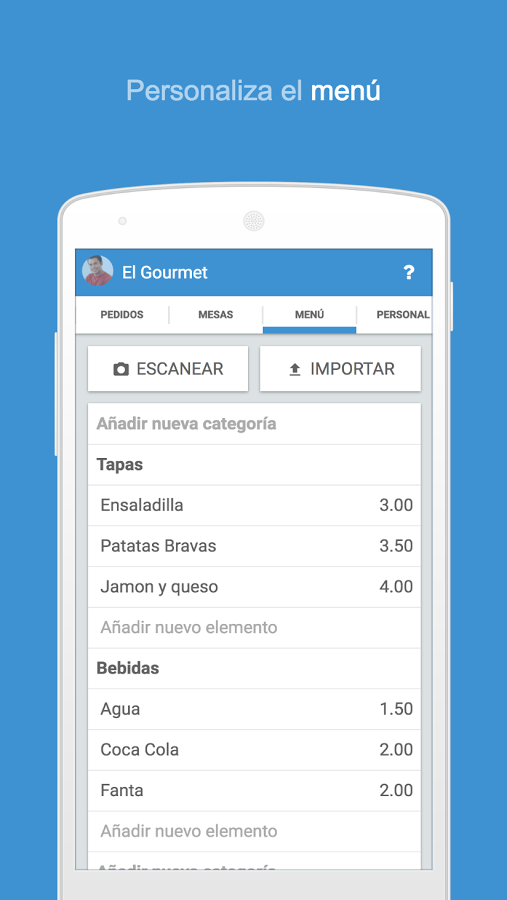
\includegraphics[scale=0.15]{Figures/waitero-1.png}
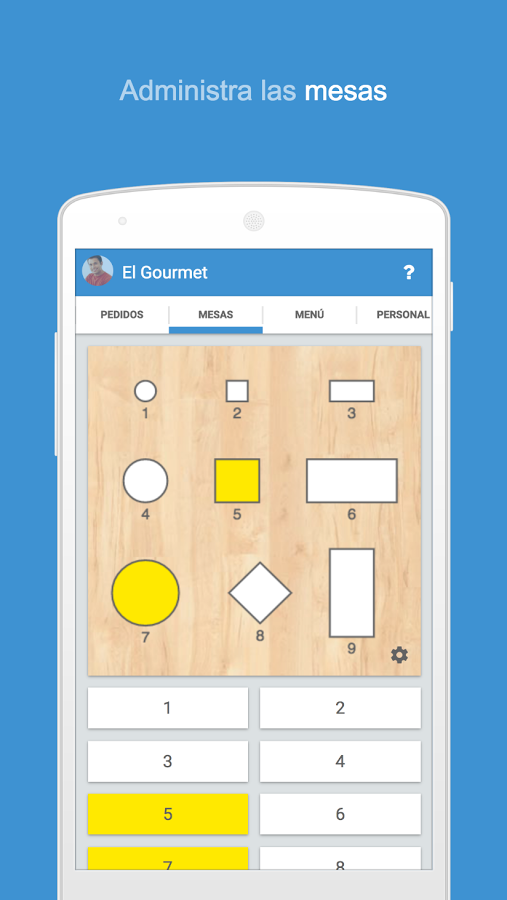
\includegraphics[scale=0.15]{Figures/waitero-2.png}
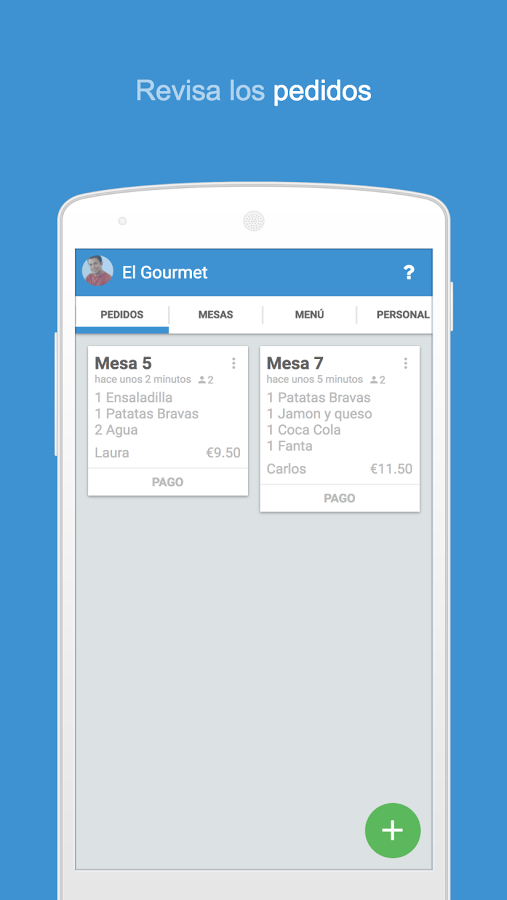
\includegraphics[scale=0.15]{Figures/waitero-3.png}
\caption{Captures de pantalla de Waitero}
\end{figure}



%----------------------------------------------------------------------------------------
%	SECTION 2
%----------------------------------------------------------------------------------------

\section{Prime Tray}

Aplicació\cite{primetray} orientada a les comandes del client a l'establiment. L'usuari té la capacitat de seleccionar un restaurant de la llista i fer la comanda en línia i anar-ho a buscar un cop és notificat.

%----------------------------------------------------------------------------------------
%	SECTION 3
%----------------------------------------------------------------------------------------

\section{OrderSev}

Aplicació\cite{ordersev} orientada especialment a substituir el TPV d'un bar o restaurant. Disposa de funcionalitats com creació de menús i comandes, generació de factures i vistes tant des de cuina com del cambrer.

%----------------------------------------------------------------------------------------
%	SECTION 4
%----------------------------------------------------------------------------------------

\section{TabletWaiter}

Aplicació\cite{tabletwaiter} orientada a ser un estil de carta per a l'establiment. Cada taula d'un restaurant hauria d'haver-hi un dispositiu amb aquesta aplicació activa a on es pugui consultar els plats i seleccionar-los, així es rebria a cuina i ja podrien començar a preparar la comanda. També permet cridar al cambrer via aplicació i demanar el compte.

%----------------------------------------------------------------------------------------
%	SECTION 5
%----------------------------------------------------------------------------------------

\section{Cloud Waiter}

Aplicació\cite{cloudwaiter} orientada a les comandes del client a l'establiment. L'usuari té la capacitat d'escanejar un codi QR amb el qual podrà accedir a l'aplicació i realitzar la comanda.

%----------------------------------------------------------------------------------------
%	SECTION 6
%----------------------------------------------------------------------------------------

\section{FastOrder}

Aplicació\cite{fastorder} orientada a les comandes del client a l'establiment. L'usuari té la capacitat d'escanejar un codi QR amb el qual podrà accedir a l'aplicació i realitzar la comanda i tot el que sigui necessari. Destacar la molt bona interfície d'usuari, que permet gaudir d'una millor experiència com a usuari.

%----------------------------------------------------------------------------------------
%	SECTION 7
%----------------------------------------------------------------------------------------

\section{Conclusions}

Encara que hi ha moltes aplicacions relacionades amb aquest àmbit (si bé, amb objectius i funcionalitats molt diverses, en alguns casos molt dispars al projecte), s'ha fet una selecció prou representativa però tot i així reduïda, amb l'objectiu de realitzar una correcta anàlisi que permeti treure conclusions de forma còmoda i eficaç.
\\\\
Un cop realitzada aquesta selecció de potencials competidors de l'aplicació, i comprès (a grans trets) les seves funcionalitats i objectius, procedim a un estudi detallat comparant-ho amb la visió d'aquest projecte.
\\\\
El que s'ha pogut veure estudiant el mercat és que hi ha dos grans grups d'aplicacions. Per una banda, tenim els sistemes que només se centren en la gestió interna de l'establiment i poder realitzar comandes més fàcil i eficientment. Per altra banda, tenim les plataformes que permeten al client, que acudeix a l'establiment, viure una millor experiència i estar còmode en la seva estança. Aleshores, partint d'aquesta premissa, \textit{Wisebite} vol innovar en el mercat oferint un nou sistema que fusioni els dos grups, així creant un fort vincle entre ambdues parts: empleat i client.
% Chapter Template

\chapter{Definició de l'abast} % Main chapter title

\label{Chapter3} % Change X to a consecutive number; for referencing this chapter elsewhere, use \ref{ChapterX}

Un sistema d'aquestes característiques podria tenir infinitat de requisits i funcionalitats, és per això que és important definir l'abast d'aquest projecte i veure quins són els objectius d'aquest.

%----------------------------------------------------------------------------------------
%	SECTION 2
%----------------------------------------------------------------------------------------

\section{Objectius}

L'objectiu principal d'aquest Treball Final de Grau és dissenyar i construir un sistema que aconsegueixi fer la vida més fàcil als empleats de qualsevol establiment de restauració, sigui bar o restaurant, i crear una millor experiència per a qualsevol usuari d'aquests locals, és a dir, millorar la seva estança oferint-li eficiència en el servei i millor tracte per part de l'establiment.
\\\\
Com ja s'ha comentat anteriorment, l'elevat cost d'implantar un sistema com aquest és la dificultat més gran. És per això que un altre objectiu important és poder construir una plataforma plenament genèrica què la puguis personalitzar al teu gust i, en definitiva, fer-la teva. Així aconseguiràs reduir una quantitat abismal en costos i obtenir majors beneficis gràcies a les funcionalitats d'aquest sistema. Perquè com bé s'ha comentat abans el cost d'implantar un sistema d'aquestes característiques no resideix en la compra d'elements tecnològics com dispositius mòbils, sinó en la compra d'un software especialitzat.
\\\\
Per altra banda es buscarà oferir la millor experiència d'usuari possible de tal manera que el cost d'aprendre a utilitzar aquesta aplicació sigui el mínim.
\\\\
Un cop especificada, dissenyada i implementada la plataforma de \textit{Wisebite} s'intentarà llançar a establiments del cercle familiar i d'amistats per així rebre un feedback de quin és el funcionament de l'aplicació en una situació real. I finalment, si la plataforma té un bon impacte, estudiar la viabilitat econòmica del projecte.

%----------------------------------------------------------------------------------------
%	SECTION 3
%----------------------------------------------------------------------------------------

\section{Abast}

En el capítol anterior s'ha analitzat les funcionalitats de les aplicacions existents en el mercat actual. En realitzar-ho, s'ha vist que totes elles es podien classificar en tres grans grups. El sistema final estarà format per aquests tres components molt importants que li donaran valor al producte resultant, i marcarà la diferència respecta la competència del mercat, tal com s'ha comentat en l'estudi anterior.

\subsection{Gestió de comandes}

En primer terme, el sistema serà capaç de gestionar les comandes d'un establiment de restauració. La plataforma tindrà la capacitat de crear menús i plats personalitzats, amb les preferències i opcions desitjades. Cadascun d'aquest contindrà informació vital i d'importància com el preu i una petita descripció del seu contingut. Com a empleat de l'establiment que té implantat \textit{Wisebite}, podrà crear comandes fàcilment i sense cap problemàtica, amb l'ajut d'una interfície molt intuïtiva. Totes les peticions seran rebudes de forma automàtica a cuina amb una interfície còmoda i agradable per tal d'agilitzar el procés el màxim possible. Aquesta informació s'anirà actualitzant en temps real sense necessitat d'actualitzar-ho manualment.
\\\\
Un cop implantat aquest component del sistema s'estarà aconseguint una millora notable en l'eficiència de les comandes. Això provocarà una satisfacció per part de la clientela, ja que rebran les comandes sol·licitades abans, que esdevindrà a uns majors ingressos per a l'establiment donat que acudirà més gent gràcies a la possible fama que es pugui generar per aquest fet.

\subsection{Anàlisi de l'establiment}

L'avantatge més important, i amb diferència, d'emmagatzemar les dades digitalment és la facilitat de realitzar un estudi detallat d'aquestes dades. El sistema tindrà la capacitat de convertir aquestes dades sense massa significat a priori a una font d'informació que serà de gran utilitat per als responsables de l'establiment.
\\\\
Per què són tan importants les dades?, es podria arribar a preguntar qualsevol. Anteriorment es prenien decisions molt importants a partir de l'experiència de les persones i de la percepció de negoci. En canvi, amb les dades en el nostre poder, es poden prendre decisions objectives i no subjectives, ja que es prenen via dades reals del consumidor. És a dir, coneixem més al nostre client.
\\\\
De forma periòdica, el sistema reportarà resums on es reflectirà informació de gran valor per a l'establiment. Informació com pot ser el tràfic setmanal, els plats més demanats, ingressos i despeses, comandes per empleat i així un llarg etcètera. Amb aquesta informació disponible esdevindrem al coneixement, és a dir, els responsables del bar o restaurant tindran la capacitat de prendre decisions a partir d'aquesta informació. Decisions que aportaran valor a l'establiment en concret i oferir un millor servei al client, així augmentant els ingressos del bar o restaurant.

\subsection{Relació amb el client}

L'última component té com a objectiu crear un fort vincle entre l'establiment i el client que hi acudeix. Qualsevol usuari d'aquesta aplicació podrà buscar l'establiment que desitgi i veure informació sobre ell com imatges, plats més demanats, valoracions i més informació que li permeti conèixer tot respecte al bar o restaurant sense necessitat d'anar-hi presencialment. Com usuari o client d'aquest establiment, tindrà la possibilitat de demanar la comanda via plataforma amb un simple escaneig d'un codi QR que haurà col·locat a cada una de les taules. Un cop acabada la visita podrà valorar el servei acompanyat de comentaris i imatges de suport per així millorar la comunitat d'usuaris de l'aplicació.
\\\\
Aquesta component aportarà flexibilitat i comoditat per a tot tipus d'usuari de l'establiment. L'atendran més ràpidament, podrà realitzar la comanda sense pressa i rumiar ben bé que és el que al final es voldrà demanar.

%----------------------------------------------------------------------------------------
%	SECTION 4
%----------------------------------------------------------------------------------------

\section{Obstacles i riscos}

Durant tot projecte, sigui de curta o llarga durada, sempre poden sorgir un seguit d'obstacles i imprevistos que poden condicionar el resultat final d'aquest, ja que té un temps limitat per construir-lo. En cas del Treball Final de Grau, estem parlant d'uns quatre mesos aproximadament.
\\\\
El principal obstacle, que pot esdevenir i serà clau de controlar, serà la gestió del temps. El Treball Final de Grau s'ha de cursar en un període limitat i s'ha d'intentar ajustar a aquest. Caldrà fer una planificació temporal el més realista possible i anar fent punts de control periòdics perquè no es descontroli l'abast del projecte i que la planificació s'adeqüi a la realitat. En cas que en aquests controls ens adonem que s'està desviant en excés es prendrà mesures segons el cas per poder-ho remeiar.
\\\\
Un altre possible obstacle que pot aparèixer és el desconeixement d'algunes tecnologies necessàries per al desenvolupament del projecte, tecnologies que s'explicaran amb més detall en capítols posteriors. Hi ha característiques i funcionalitats que tindrà el sistema que requereixen uns coneixements tècnics per a poder-les fer realitat, les quals no disposa l'autor del projecte en nivell expert. Pot donar-se el cas també que en realitzar la planificació temporal d'una tasca es calculi un temps X que finalment no es podrà complir donat el desconeixement exacte del cost corresponent, ja que no es desconeixia la tecnologia.
\\\\
Un altre inconvenient o imprevist que pot sorgir és una gran quantitat d'errors en el codi durant la fase d'implementació del projecte. Sempre solen aparèixer nombrosos errors durant el desenvolupament d'un projecte, però solen haver-hi alguns que requereixen una dedicació extra per solucionar-los. S'ha de saber filtrar quins errors són vitals de solucionar i quins es poden evitar i esquivar-los.
\\\\
I finalment pot donar-se el cas, tot i ser molt remot, que alguns dels serveis externs que utilitza la plataforma quedin inhabilitats durant un període que dificulti el desenvolupament i testeig de l'aplicació.
\\\\
Tots aquests possibles problemes que poden sorgir durant el període d'aquest Treball Final de Grau han de ser tractats immediatament de tal manera que no es converteixin en problemes crítics difícils de solucionar. El pla d'acció per solucionar-los en cas que passin es comentarà de forma més detallada en capítols posteriors.

%----------------------------------------------------------------------------------------
%	SECTION 5
%----------------------------------------------------------------------------------------

\section{Metodologia i rigor}

Durant el transcurs de la carrera, i en especial l'especialitat d'Enginyeria del Software, he après un seguit de metodologies de treball però, sense dubte, em quedaria amb tot el grup de tècniques que engloben les metodologies àgils. En conseqüència, aquest projecte seguirà una metodologia àgil, en concret una inspirada en la metodologia \textit{Scrum}.
\\\\
Inicialment, en les primeres setmanes esdevindrà la Fase Inicial del projecte, que ve a ser l'assignatura de Gestió de Projectes (\textit{GEP}). En ella s'especificarà tot el necessari per al sistema que es vol construir. En concret, s'especificarà per un cantó la definició de l'abast i la contextualització del projecte, per altra banda la planificació temporal i finalment la gestió econòmica i de sostenibilitat. A més a més, per tal de situar-se en el punt inicial i poder fer una petita prova de com pot arribar a ser la lectura final, es realitzarà una presentació de cinc minuts explicant el realitzat en aquesta fase inicial.
\\\\
Un cop tot especificat vindrà la fase intermèdia del projecte, dit d'altra manera, la fase de desenvolupament d'aquest. En ella es crearan un seguit d'\textit{Sprints}, seguint la metodologia àgil, d'unes dues setmanes de duració que s'analitzaran en una retrospectiva posterior amb el director del projecte. Amb aquests \textit{Sprints} serà fàcil validar la feina feta i veure com va el projecte, és a dir, si la planificació inicial realitzada s'adequa al pas del projecte. Cada una d'aquests \textit{sprints} contindrà un conjunt d'\textit{Històries d'usuari} que representaran la feina a realitzar durant aquelles dues setmanes. Una \textit{història d'usuari} es pot entendre com una petita part funcional d'un projecte, és a dir, una funcionalitat d'aquest. La gràcia de dividir-ho en històries d'usuari és poder separar tota la feina que comporta un projecte en tasques molt petites i, a priori, independent entre elles. A més a més, a cada una d'aquestes històries d'usuari se li atribuirà una puntuació que representarà el cost d'implementació d'aquestes, per així poder prioritzar-les segons la disponibilitat del moment.
\\\\
A la vegada es registrarà totes les accions que es van fent per controlar quant temps es tarda a realitzar cada una de les tasques que es planteja fer. Així, en cada una de les retrospectives, es podrà analitzar si les puntuacions atorgades a cada una de les targetes o bé històries d'usuari són correctes o no.
\\\\
S'estipularà una nomenclatura i unes convencions fixes durant el desenvolupament del projecte per així tenir un millor control de quines històries d'usuari s'estan realitzant en aquell precís moment i, en general, disposar d'un historial de desenvolupament amb un format únic. Així doncs, en finalitzar la implementació es disposarà d'un codi net i que simplement llegint-ho s'entendrà el seu funcionament.

\subsection{Metodologia de desenvolupament: convencions de git}
\textbf{Commits}
\\
Missatges en anglès i en minúscules començant per un verb comú com per exemple "\textit{add}", "\textit{remove}", "\textit{update}", "\textit{refactor}", "\textit{fix}" o un qualsevol altre, que descrigui en poques paraules l'acció realitzada en el commit, així serà clar el que s'ha modificat sense necessitat d'entrar a veure els canvis.
\\\\
\textbf{Feature branch workflow}
\\
Model de desenvolupament basat en les "\textit{branches}" (branques) de git. Ajuda a realitzar un desenvolupament incremental del producte, fomenta la cronologia del codi i minimitza els possibles conflictes entre versions quan es desenvolupen. S'utilitza un repositori central com a història oficial del projecte, història que funciona sense cap tipus d'error. Internament, s'usen 2 tipologies de "\textit{branch}":
\begin{itemize}
\item \textit{Master branch}: és on està l'historial de codi acceptat i acabat del projecte. És única. Tot funciona dins d'aquesta branca.
\item \textit{Feature branches}: branches separades de la master on es realitzen els commits per desenvolupar una història d'usuari del projecte o per resoldre un problema oposat. El nom ha de ser descriptiu sobre el que s'està desenvolupant perquè al llegir-ho es sàpiga què es tracta en aquesta branch.
\end{itemize}
Una vegada acabat el desenvolupament en un feature branch s'inicia una Pull request, explicat posteriorment, per ajuntar-la amb la branca principal anomenada master. Així doncs aconsegueixes separar la part de codi funcional amb la que ho acabarà sent.
\\\\
\textbf{Pull requests}
\\
Una pull request és una conversa sobre els canvis realitzats en una branch abans d'ajuntar-ho amb la base genèrica de codi que és la branch master. Això afavoreix una revisió del codi per evitar possibles problemes amb aquell fragment modificat o afegit. I a més poder documentar d'alguna manera el transcurs o evolució del codi.

\subsection{Metodologia de desenvolupament: gestió de tiquets}
Cada vegada que s'hagi detectat algun problema en el codi de l'aplicació que està en la branca principal master s'obrirà un "\textit{issue}" en GitHub, portal que s'explicarà amb deteniment en capítols posteriors. Per tancar-ho o esmentar-ho s'aprofitarà la sintaxi pròpia de GitHub amb els commits:
\begin{itemize}
\item \textit{Closes \#12} (on 12 és el nombre del issue corresponent). Amb un commit que té aquest missatge aconseguim tancar el "\textit{issue}" determinat.
\item \textit{\#12} (on 12 és el nombre del issue corresponent). Amb un missatge d'aquest estil aconseguim referir a el "issue" indicat.
\end{itemize}

\subsection{Metodologia de desenvolupament: trello}
Per gestionar el projecte seguirem Trello a causa de la seva semblança a les metodologies àgils. El flux de les històries d'usuari passarà per dos taulers dins l'aplicació Trello:
\begin{itemize}
\item \textit{Backlog}: tauler únic durant tot el projecte. És el punt d'entrada de qualsevol requisit del projecte. Té 3 llistes, per les quals les històries han d'anar passant abans de poder ser assignades a un sprint. Aquestes llistes corresponen a les diferents fases d'especificació fins que és cada una de les històries d'usuari està totalment definida per tal de ser llançada a algun dels sprints del projecte.
\begin{itemize}
\item Història d'usuari genèrica
\item Història d'usuari amb criteris d'acceptació
\item Història d'usuari amb criteris d'acceptació i punts d'història
\end{itemize}
\item \textit{Taulers de Sprint}: taulers propis, per cada un dels cinc sprints que tindrà el projecte, on s'afegeixen les històries a realitzar que s'hagin decidit en el \textit{Sprint Planning}, considerant aquest concepte com el fet de decidir quines de les històries d'usuari del backlog van a aquesta iteració. Aquestes històries han de sortir del backlog, de la llista d'històries estimades. Per facilitar i uniformar la creació d'aquests taulers, existeix una plantilla de tauler de trello del que es realitzarà una còpia per crear cada tauler. Una vegada copiat es personalitza segons les necessitats d'aquest sprint durant el \textit{Sprint Planning}. Aquesta plantilla podrà ser modificada a final de cada sprint en la retrospectiva, per poder millorar el flux de treball intern de cada sprint.
\end{itemize}

\subsection{Metodologia de desenvolupament: codi Java}
Per desenvolupar en Java, ja que la tecnologia Android s'escriu en aquest llenguatge de programació, es seguirà una convenció de noms comú en Java segons estipula la comunitat de desenvolupadors.
\begin{itemize}
\item \textit{Funcions i variables}: Escrites en el format CamelCase\cite{camelcase} amb la primera lletra en minúscula.
\item \textit{Constant}: Escrites en majúscules i separant paraules amb “\_”.
\item \textit{Classes}: Escrites en el format CamelCase amb la primera lletra en majúscula.
\item \textit{Paquets}: Escrits en minúscula i una sola paraula.
\item \textit{Documentació}: Seguirem el format de JavaDoc\cite{javadoc}.
\end{itemize}
% Chapter Template

\chapter{Anàlisi de requisits} % Main chapter title

\label{Chapter4} % Change X to a consecutive number; for referencing this chapter elsewhere, use \ref{ChapterX}

%----------------------------------------------------------------------------------------
%	SECTION 1
%----------------------------------------------------------------------------------------

\section{Agents implicats}
En tot projecte en el qual ens podem trobar, inclòs un treball final de grau com en el que ens trobem, un conjunt o col·lectiu de persones afectades de forma directa o indirecte.
\\\\
En concret, en el que es refereix \textit{Wisebite}, destaca en especial un dels punts comentats en capítols anteriors. Dins les tres problemàtiques per les quals els usuaris no disposaven d'una implantació d'un sistema de gestió en el seu establiment de restauració és per l'elevat cost que té, és a dir, el problema ve degut per un factor econòmic. Aquest col·lectiu de persones que es veuen dins d'aquesta problemàtica no és pas un grup petit, sinó tot el contrari. És per això que és molt important valorar en aquest projecte quins són els agents implicats.
\\\\
Les parts interessades o stakeholders\cite{stakeholder} d'un projecte són aquelles persones o agrupacions de persones que el projecte els afecta de manera directa o indirecta. Aquests grups poden tenir objectius totalment diferents entre ells, i que cada part interessada jugui un paper clau en el desenvolupament i vida del projecte. Per això és important destacar cada una d'elles.

\subsection{Director del projecte}
En trobar-nos en un Treball Final de Grau, apareix la figura del director. En \textit{Wisebite}, el director és l'Ernest Teniente\cite{ernestteniente}, actualment professor de la Universitat Politècnica de Catalunya. Va ser el primer contacte quant a la inscripció del projecte i és el responsable de guiar a l'autor del projecte durant tot el transcurs d'aquest i supervisar tots els punts que vegi necessaris. Guiarà a l'autor del projecte i facilitarà tots els seus recursos disponibles per a poder construir un bon treball conjuntament amb l'autor d'aquest.

\subsection{Equip desenvolupador}
El grup de desenvolupadors del projecte són un dels actors més importants, per no dir el més important, ja que aporta la capacitat de convertir la idea teòrica a la pràctica. Al parlar d'un treball final de grau, l'equip de desenvolupadors es redueix a una sola persona, l'estudiant i autor d'aquest.
\\\\
Aquesta persona té com a objectiu iniciar i llançar el projecte endavant, passant per tot el procés d'inscripció de treball. Un cop passada aquesta etapa, l'equip desenvolupador ha de dissenyar i perfeccionar la idea, definir-la, implementar-la i documentar-la per així poder-la presentar en la fase final del treball.

\subsection{Establiments de restauració}
Com s'ha comentat anteriorment, l'aparició de \textit{Wisebite} té com a objectiu principal convertir i fer evolucionar el món de la restauració. L'aparició de sistemes com aquest aporta un gran canvi a aquest sector. Els responsables de cada un dels establiments disponibles al mercat tindran la possibilitat d'implantar aquest projecte al seu negoci amb l'objectiu de millorar els resultats.
\\\\
El paper, i la reacció que esdevingui d'aquest col·lectiu, en conèixer l'aparició de \textit{Wisebite} serà de gran importància per definir el futur de la plataforma. Ens podem trobar amb la situació que l'aplicació guanyi gran fama i es faci un bon lloc dins d'aquest sector, o bé oposadament que acabi passant desapercebuda dins de la restauració. Aquest futur es decideix en la reacció d'aquest col·lectiu.

\subsection{Clients}
Si un establiment, sigui bar o restaurant, decideix implantar aquest sistema, no només canviarà la perspectiva de l'empleat sinó també del client o usuari. El comportament que realitzava anteriorment en entrar a aquest establiment haurà de canviar una mica per adaptar-se al nou sistema implantat.
\\\\
En primera instància, podrà observar com la gestió de comandes dels cambrers ha canviat de forma dràstica i que tota la gestió del restaurant en general ha evolucionat. Per altra banda, com s'ha mencionat en l'abast del projecte, tu com a usuari de \textit{Wisebite} no et fa falta pertànyer a un restaurant determinat en utilitzar l'aplicació, sinó que també pots interactuar amb la plataforma amb el perfil de client, és a dir, cercant els restaurants de la zona, consultar els seus detalls i fins i tot poder realitzar comandes des del seu propi terminal a una taula especificada.
\\\\
En conseqüència, aquí els clients pertanyents a aquests establiments de restauració són un altre col·lectiu molt important en el transcurs de la història de \textit{Wisebite}.

\subsection{Competència}
Els propietaris i responsables de sistemes similars al d'aquest projecte veuran amenaçada la seva idea i projecció de negoci, propietaris com els de les plataformes i aplicacions comentades en l'estudi de mercat de capítols anteriors.
\\\\
Aquests altres sistemes poden comportar-se de dues maneres diferents i oposades entre si. Per una banda, podrien aportar millores als seus respectius projectes per així oferir una millor plataforma als usuaris d'aquesta, ja sigui des del perfil treballador com client. O bé per altra banda ignorar-ho i mantenir el seu pla de negoci. Fet que podria fer destacar \textit{Wisebite} com la diferent dins del sector i fer-la important en aquest.
\\\\
Així doncs, igual que els altres col·lectius, aquest té una importància diferent però igual d'important pel paper que hi juga en l'evolució i futur de la plataforma.


%----------------------------------------------------------------------------------------
%	SECTION 2
%----------------------------------------------------------------------------------------

\section{Requisits funcionals}

A \textit{Wisebite}, com en tot projecte, es disposa d'un seguit de requisits funcionals o funcionalitats que defineixen l'ús de la plataforma. El conjunt de tots ells engloben totes les possibilitats de les quals disposa l'usuari en interaccionar amb l'aplicació.

\begin{enumerate}
\item \textbf{Iniciar sessió}: es permetrà iniciar sessió amb algun dels comptes de \textit{Google} de les quals disposa l'usuari.
\item \textbf{Tancar sessió}: es permetrà tancar sessió del sistema.
\item \textbf{Veure usuari}: es permetrà veure o consultar els detalls del teu usuari obtenint el nom, el cognom, el correu electrònic, la localització, el nom del restaurant al qual està relacionat (si escau) i el nombre de comandes realitzades (si existeixen), a més de la imatge de perfil.
\item \textbf{Editar informació bàsica d'usuari}: es permetrà editar la informació bàsica de l'usuari, englobant el nom, el cognom i la localització.
\item \textbf{Canviar imatge de perfil}: es permetrà editar la imatge de perfil permetent pujar una imatge nova emmagatzemada al dispositiu de l'usuari.
\item \textbf{Crear restaurant}: es permetrà la creació d'un establiment de restauració indicant tota la informació necessària: nom, localització, descripció, telèfon de contacte, pàgina web, nombre de taules, horaris d'apertura i la carta de plats i menús dels quals disposa el bar o restaurant.
\item \textbf{Consultar restaurant}: es permetrà obtenir tota la informació referent al restaurant en qüestió, podent-se així informar sobre l'establiment.
\item \textbf{Crear una comanda al teu restaurant}: es permetrà crear una comanda al teu restaurant especificant la taula en la qual es realitza la comanda, i el conjunt de plats i menús que ha especificat el client.
\item \textbf{Obtenir les comandes actives}: es permetrà llistar el conjunt de comandes actives dins del teu restaurant, és a dir, totes les comandes les quals encara no han estat cobrades completament, podent veure el percentatge d'elements preparats, entregats i cobrats.
\item \textbf{Consultar l'estat d'una comanda}: es permetrà consultar els detalls de la comanda seleccionada. Els detalls constituiran tots els elements que formen la comanda, podent veure si s'ha preparat, entregat i/o cobrat cadascun dels elements.
\item \textbf{Cancel·lar una comanda}: es permetrà cancel·lar la comanda, així eliminant tota instància d'aquesta.
\item \textbf{Consultar els plats que encara no han estat preparats}: es permetrà obtenir tots els plats que encara no han estat preparats dins del teu restaurant per així poder filtrar-ho pels integrants de la cuina.
\item \textbf{Marcar la realització d'un plat}: es permetrà indicar la realització d'un plat per així emmagatzemar-ho al sistema i deixar-ho enregistrat.
\item \textbf{Marcar l'entrega d'un plat}: es permetrà indicar l'entrega d'un plat per així emmagatzemar-ho al sistema i deixar-ho enregistrat.
\item \textbf{Cobrar una comanda de forma total}: es permetrà cobrar una comanda específica recol·lectant el total de la comanda en qüestió.
\item \textbf{Cobrar una comanda de forma fraccionada}: es permetrà cobra una comanda de forma fraccionada, és a dir, seleccionar un subconjunt dels elements de la comanda per així cobrar-ho de forma separada.
\item \textbf{Afegir un usuari al restaurant}: es permetrà afegir un usuari a un establiment en específic per així donar-li accés a totes les funcionalitats d'aquest.
\item \textbf{Obtenir les estadístiques del teu restaurant}: es permetrà veure les estadístiques del teu establiment de restauració consultant el nombre de comandes, el preu mitjà d'aquestes, el total obtingut, el millor i pitjor plat, el millor i pitjor menú, la millor franja horària, el temps mitjà entre l'inici i el final d'una comanda, la puntuació mitjana i el comptador de valoracions. A més d'anar acompanyat de tres gràfiques que especifiquen el percentatge de plats i menús venuts, i les franges horàries. Totes aquestes dades seran filtrades per dia, setmana o mes.
\item \textbf{Canviar la data de l'anàlisi}: es permetrà canviar la data de l'anàlisi i situar-se en un dia desitjat i consultar les estadístiques d'aquell dia, d'aquella setmana i d'aquell mes.
\item \textbf{Llistar tots els restaurants}: es permetrà llistar tots els restaurants de la plataforma podent veure els dies d'apertura, el nombre de plats i menús i la valoració mitjana de cadascun d'ells.
\item \textbf{Crear una comanda a un restaurant aliè}: es permetrà crear una comanda a un restaurant diferent del de la propietat de l'usuari, en cas que existeixi, especificant tota la informació necessària.
\item \textbf{Consultar les valoracions pendents}: es permetrà consultar les valoracions pendents de les quals disposarà l'usuari en qüestió.
\item \textbf{Valorar una comanda}: es permetrà valorar una comanda en concret indicant la puntuació dels plats i menús demanats, acompanyats d'un comentari opcional. A més a més, es permetrà valorar de forma global l'opinió sobre el restaurant.
\item \textbf{Consultar les valoracions d'un plat o menú}: es permetrà obtenir les valoracions d'un plat o menú per així veure l'opinió d'aquest.
\item \textbf{Consultar les valoracions d'un restaurant}: es permetrà obtenir les valoracions d'un restaurant en concret per així veure l'opinió d'aquest.
\end{enumerate}
\newpage

%----------------------------------------------------------------------------------------
%	SECTION 3
%----------------------------------------------------------------------------------------

\section{Requisits no funcionals}

En aquest apartat es realitzarà un repàs de tots els requisits no funcionals\cite{requisito} o de qualitat dels quals disposa el sistema, és a dir, l'especificació de quelcom sobre el mateix sistema, i de com s'ha de realitzar les accions pertinents a aquest. Per entendre-ho amb més facilitat s'ha dividit el conjunt de requisits segons el tipus descrit per \textit{Volere}\cite{volere}.
\\\\
% ONE
\noindent\textbf{Requisits d'aparença}
\begin{itemize}
\item \textit{Tipus de requisit (Volere)}: 10a
\item \textit{Descripció}: Disseny atractiu i d'ús senzill que convidarà a l'usuari a fer-ne ús amb més facilitat.
\item \textit{Justificació del requisit}: Com l'aplicació treballa sobre un nombre de persones considerable, com és tot el sector de la restauració i els seus respectius clients, cal destacar per l'atractiu de l'aplicació per tal de marcar un abans i un després en l'usuari, és a dir, que gaudeixi de l'experiència a l'hora d'utilitzar \textit{Wisebite}.
\item \textit{Condició de satisfacció}: El requisit se satisfarà si s'obté una bona valoració dels usuaris en respecte a l'aparença. Es podrà verificar amb una enquesta de satisfacció al conjunt d'usuaris de l'aplicació.
\end{itemize}

% TWO
\noindent\textbf{Requisits d'estil}
\begin{itemize}
\item \textit{Tipus de requisit (Volere)}: 10b
\item \textit{Descripció}: Disseny modern i ambiciós, seguint la tendència en disseny però destacant en punts específics.
\item \textit{Justificació del requisit}: La competència del mercat ens obliga a disposar d'un disseny modern per tal destacar sobre la comunitat d'usuaris, i així guanyar usuaris no només per les funcionalitats de la plataforma, sinó per l'estil de l'aplicació.
\item \textit{Condició de satisfacció}: El requisit se satisfarà si més de tres quartes parts dels usuaris consideren que \textit{Wisebite} disposa d'un disseny modern, fet que es podrà comprovar amb una enquesta.
\end{itemize}

% THREE
\noindent\textbf{Requisits de facilitat d'ús}
\begin{itemize}
\item \textit{Tipus de requisit (Volere)}: 11a
\item \textit{Descripció}: El sistema ha de ser intuïtiu i fàcil d'usar. Complirà els criteris en temes de disseny, de contingut, d'estructura i de presentació fixats pel W3C\cite{w3c}.
\item \textit{Justificació del requisit}: Un punt diferenciador important és que l'usuari pugui fer servir el sistema intuïtivament, de manera que no perdi el temps intentant descobrir com funciona i, a més a més, que qualsevol persona sigui capaç de familiaritzar-se amb el sistema. Aquest fet és molt important, ja que la majoria dels usuaris de \textit{Wisebite} no formarà part de la comunitat dels informàtics.
\item \textit{Condició de satisfacció}: El requisit se satisfarà si un usuari amb poca experiència en aplicacions aconsegueix usar-lo sense cap problema. Per això, s'utilitzarà un grup de persones inexpert en l'ús d'aplicacions mòbil per veure quina és la seva reacció utilitzant \textit{Wisebite}.
\end{itemize}

% FOUR
\noindent\textbf{Requisits de latència i velocitat}
\begin{itemize}
\item \textit{Tipus de requisit (Volere)}: 12a
\item \textit{Descripció}: La resposta del sistema ha de ser de menys d'un segon com a mínim en el 95\% de les operacions.
\item \textit{Justificació del requisit}: Un temps de resposta ràpid permet que l'usuari no perdi el flux o atenció del que està fent amb el sistema. Una plataforma de latència i velocitat dolenta produiria insatisfacció per part de l'usuari.
\item \textit{Condició de satisfacció}: El requisit se satisfarà si donat un estudi sobre el rendiment de l'aplicació, aquest confirma que el temps d'espera en cada acció és menor al segon en el 95\% dels casos.
\end{itemize}

% FIVE
\noindent\textbf{Requisits de precisió o exactitud}
\begin{itemize}
\item \textit{Tipus de requisit (Volere)}: 12c
\item \textit{Descripció}: Totes les dates que s'incloguin en l'aplicació tindran el format universal: \textit{DD/MM/AAAA}
\item \textit{Justificació del requisit}: És convenient especificar el format de la data, ja que no a tot arreu té el mateix format i podria provocar malentesos i confusions entre els usuaris.
\item \textit{Condició de satisfacció}: El requisit se satisfarà si el format de la data i l'hora segueix l'estàndard ISO-8601\cite{iso8601} extens d'estil Europeu (EN 28601).
\end{itemize}

% SIX
\noindent\textbf{Requisit de disponibilitat}
\begin{itemize}
\item \textit{Tipus de requisit (Volere)}: 12d
\item \textit{Descripció}: El sistema haurà d'estar disponible les 24 hores del dia durant els 365 dies que conformen l'any.
\item \textit{Justificació del requisit}: Els usuaris han de poder utilitzar el sistema en qualsevol moment del dia per tal de poder buscar restaurants o gestionar-los.
\item \textit{Condició de satisfacció}: El requisit se satisfarà si el sistema està disponible i completament funcional tot el temps.
\end{itemize}

% SEVEN
\noindent\textbf{Requisits d'adaptabilitat}
\begin{itemize}
\item \textit{Tipus de requisit (Volere)}: 14c
\item \textit{Descripció}: L'aplicació mòbil ha de poder-se veure i executar correctament en els diferents smartphones del mercat, i tenir les mateixes funcionalitats i característiques en tots ells.
\item \textit{Justificació del requisit}: L'existència de tants telèfons mòbils diferents i tantes versions d'Android disponibles actualment obliga a garantir que com a mínim es veurà de forma correcta i es podrà executar totes les funcionalitats de la plataforma.
\item \textit{Condició de satisfacció}: El requisit se satisfarà si el sistema es pot visualitzar i executar correctament en els principals smartphones del mercat.
\end{itemize}

% EIGHT
\noindent\textbf{Requisit d'immunitat}
\begin{itemize}
\item \textit{Tipus de requisit (Volere)}: 15e
\item \textit{Descripció}: El sistema està protegit d'atacs externs i infeccions per software maliciós.
\item \textit{Justificació del requisit}: S'ha de garantir la seguretat per evitar posar en risc la disponibilitat del sistema i la privadesa de les dades dels usuaris. Avui en dia que tot està tan digitalitzat, és un fet molt important per garantir la comoditat de l'usuari a l'hora d'accedir a la plataforma.
\item \textit{Condició de satisfacció}: El requisit se satisfarà si s'implementa la normativa de seguretat internacional ISO-17799\cite{iso17799} per tal de garantir la seguretat davant d'atacs externs.
\end{itemize}

% NINE
\noindent\textbf{Requisits legals}
\begin{itemize}
\item \textit{Tipus de requisit (Volere)}: 17a
\item \textit{Descripció}: S'aconseguiran tots els drets sobre els serveis externs que s'utilitzin a l'aplicació i a la vegada es compliran les lleis sobre el tractament de dades personals.
\item \textit{Justificació del requisit}: Es pactaran acords amb totes les empreses de les quals s'utilitzen els seus serveis, arribant a acords sigui amb la Universitat per poder aprofitar la seva plataforma o amb empreses externes. I també mostrar transparència a l'hora de no compartir dades personals per fins no vinculants al sistema.
\item \textit{Condició de satisfacció}: El requisit se satisfarà si no es rep cap denuncia per part de cap servei extern, ni de cap usuari per ús indegut de les dades personals.
\end{itemize}


%----------------------------------------------------------------------------------------
%	SECTION 4
%----------------------------------------------------------------------------------------

\newpage
\section{Casos d'ús}

Un cop definits i analitzats tots els requisits del sistema, caldrà explicar i especificar els casos d'ús de la plataforma. Per realitzar-ho, s'ha decidit dividir els vint-i-cinc casos d'ús en diferents categories segons el tipus de funcionalitat que vol aconseguir el cas d'ús en concret. El conjunt de casos d'ús es dividirà quatre grups: gestió d'usuaris, gestió de l'establiment, anàlisi de l'establiment i interacció del client.

\subsection{Gestió d'usuaris}
\begin{figure}[H]
\centering
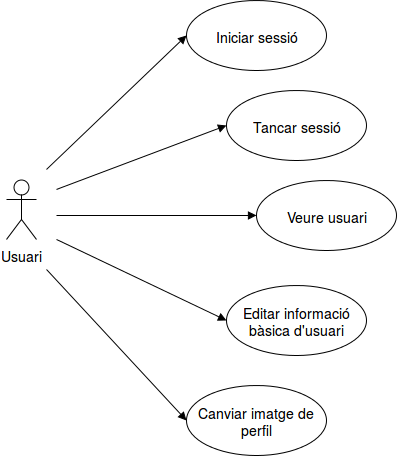
\includegraphics[scale=0.6]{Figures/casosUs_gestioUsuaris.png}
\caption{Diagrama de casos d'ús referent a la gestió d'usuaris}
\end{figure}

\begin{table}[!h]
\centering
\begin{tabular}{|l|L|l|}
\hline
\textbf{Cas d'ús}& \#1 & Iniciar sessió \\ \hline
\textbf{Actor principal} & \multicolumn{2}{l|}{Usuari} \\ \hline
\textbf{Precondició} & \multicolumn{2}{M|}{L'usuari ha accedit a la primera pantalla de l'aplicació.} \\ \hline
\textbf{Trigger} & \multicolumn{2}{M|}{L'usuari vol iniciar sessió al sistema.} \\ \hline
\multicolumn{3}{|T|}{\textbf{Escenari principal d'èxit}} \\ \hline
\multicolumn{3}{|T|}{1. L'usuari clica al botó d'iniciar sessió.}\\
\multicolumn{3}{|T|}{2. El sistema redirigeix l'usuari al llistat de comptes de Google disponibles al dispositiu.}\\
\multicolumn{3}{|T|}{3. L'usuari selecciona el compte desitjat.}\\
\multicolumn{3}{|T|}{4. El sistema redirigeix a l'usuari a la pantalla principal de l'aplicació, ja amb la sessió iniciada.}\\
\hline
\end{tabular}
\label{}
\caption{Cas d'ús \textit{Iniciar sessió}}
\end{table}

\begin{table}[!h]
\centering
\begin{tabular}{|l|L|l|}
\hline
\textbf{Cas d'ús}& \#2 & Tancar sessió \\ \hline
\textbf{Actor principal} & \multicolumn{2}{l|}{Usuari} \\ \hline
\textbf{Precondició} & \multicolumn{2}{M|}{L'usuari ha accedit a la pantalla principal de l'aplicació.} \\ \hline
\textbf{Trigger} & \multicolumn{2}{M|}{L'usuari vol tancar sessió al sistema.} \\ \hline
\multicolumn{3}{|T|}{\textbf{Escenari principal d'èxit}} \\ \hline
\multicolumn{3}{|T|}{1. L'usuari clica sobre la icona de la cantonada esquerra de la barra superior.}\\
\multicolumn{3}{|T|}{2. El sistema mostra a l'usuari un desplegable amb l'opció de tancar sessió.}\\
\multicolumn{3}{|T|}{3. L'usuari clica sobre l'opció de tancar sessió}\\
\multicolumn{3}{|T|}{4. El sistema redirigeix a l'usuari a la primera pantalla de l'aplicació, ja amb la sessió tancada}\\
\hline
\end{tabular}
\label{}
\caption{Cas d'ús \textit{Tancar sessió}}
\end{table}

\begin{table}[!h]
\centering
\begin{tabular}{|l|L|l|}
\hline
\textbf{Cas d'ús}& \#3 & Veure usuari \\ \hline
\textbf{Actor principal} & \multicolumn{2}{l|}{Usuari} \\ \hline
\textbf{Precondició} & \multicolumn{2}{M|}{L'usuari ha accedit a la pantalla principal de l'aplicació.} \\ \hline
\textbf{Trigger} & \multicolumn{2}{M|}{L'usuari vol accedir a la seva informació.} \\ \hline
\multicolumn{3}{|T|}{\textbf{Escenari principal d'èxit}} \\ \hline
\multicolumn{3}{|T|}{1. L'usuari clica sobre el \textit{Navigational drawer} amb l'objectiu de fer-lo desplegar.}\\
\multicolumn{3}{|T|}{2. El sistema desplega el menú lateral.}\\
\multicolumn{3}{|T|}{3. L'usuari clica sobre la seva imatge situada a la part superior del menú lateral.}\\
\multicolumn{3}{|T|}{4. El sistema redirigeix a l'usuari a la pantalla de detall d'usuari.}\\
\hline
\end{tabular}
\label{}
\caption{Cas d'ús \textit{Veure usuari}}
\end{table}

\begin{table}[!h]
\centering
\begin{tabular}{|l|L|l|}
\hline
\textbf{Cas d'ús}& \#4 & Editar informació bàsica d'usuari \\ \hline
\textbf{Actor principal} & \multicolumn{2}{l|}{Usuari} \\ \hline
\textbf{Precondició} & \multicolumn{2}{M|}{L'usuari ha accedit a la pantalla de detall de l'usuari.} \\ \hline
\textbf{Trigger} & \multicolumn{2}{M|}{L'usuari vol modificar la seva informació bàsica.} \\ \hline
\multicolumn{3}{|T|}{\textbf{Escenari principal d'èxit}} \\ \hline
\multicolumn{3}{|T|}{1. L'usuari clica sobre el botó rodó de la dreta de la part inferior de la pantalla.}\\
\multicolumn{3}{|T|}{2. El sistema redirigeix a l'usuari a la pantalla d'editar usuari.}\\
\multicolumn{3}{|T|}{3. L'usuari modifica algun o alguns dels tres camps que té disponibles: nom, cognom i localització. L'usuari clica sobre el botó superior de la dreta per confirmar els canvis.}\\
\multicolumn{3}{|T|}{4. El sistema emmagatzema els canvis i redirigeix a l'usuari a la pantalla de detall d'usuari.}\\
\hline
\multicolumn{3}{|T|}{\textbf{Extensions}} \\ \hline
\multicolumn{3}{|T|}{2.a L'usuari cancel·la els canvis} \\
\multicolumn{3}{|T|}{\tab2.a.1 L'usuari clica sobre la marxa enrere de la barra superior.} \\
\multicolumn{3}{|T|}{\tab2.a.2 El sistema redirigeix a l'usuari a la pantalla de detall de l'usuari sense cap canvi emmagatzemat.} \\\hline
\end{tabular}
\label{}
\caption{Cas d'ús \textit{Editar informació bàsica d'usuari}}
\end{table}

\begin{table}[!h]
\centering
\begin{tabular}{|l|L|l|}
\hline
\textbf{Cas d'ús}& \#5 & Canviar imatge de perfil \\ \hline
\textbf{Actor principal} & \multicolumn{2}{l|}{Usuari} \\ \hline
\textbf{Precondició} & \multicolumn{2}{M|}{L'usuari ha accedit a la pantalla de detall de l'usuari.} \\ \hline
\textbf{Trigger} & \multicolumn{2}{M|}{L'usuari vol modificar la seva imatge de perfil.} \\ \hline
\multicolumn{3}{|T|}{\textbf{Escenari principal d'èxit}} \\ \hline
\multicolumn{3}{|T|}{1. L'usuari clica sobre el botó rodó de la dreta de la part inferior de la pantalla.}\\
\multicolumn{3}{|T|}{2. El sistema redirigeix a l'usuari a la pantalla d'editar usuari.}\\
\multicolumn{3}{|T|}{3. L'usuari clica sobre la imatge d'usuari.}\\
\multicolumn{3}{|T|}{4. El sistema mostra la galeria amb les imatges disponibles dins del dispositiu.}\\
\multicolumn{3}{|T|}{5. L'usuari selecciona la imatge desitjada.}\\
\multicolumn{3}{|T|}{6. El sistema redirigeix a la pantalla d'editar usuari amb la imatge modificada per la seleccionada.}\\
\multicolumn{3}{|T|}{7. L'usuari clica sobre el botó superior de la dreta per confirmar els canvis.}\\
\multicolumn{3}{|T|}{8. El sistema emmagatzema els canvis i redirigeix a l'usuari a la pantalla de detall d'usuari.}\\
\hline
\multicolumn{3}{|T|}{\textbf{Extensions}} \\ \hline
\multicolumn{3}{|T|}{2.a L'usuari cancel·la els canvis} \\
\multicolumn{3}{|T|}{\tab2.a.1 L'usuari clica sobre la marxa enrere de la barra superior.} \\
\multicolumn{3}{|T|}{\tab2.a.2 El sistema redirigeix a l'usuari a la pantalla de detall de l'usuari sense cap canvi emmagatzemat.} \\
\multicolumn{3}{|T|}{6.a L'usuari cancel·la els canvis} \\
\multicolumn{3}{|T|}{\tab6.a.1 L'usuari clica sobre la marxa enrere de la barra superior.} \\
\multicolumn{3}{|T|}{\tab6.a.2 El sistema redirigeix a l'usuari a la pantalla de detall de l'usuari sense cap canvi emmagatzemat.} \\\hline
\end{tabular}
\label{}
\caption{Cas d'ús \textit{Canviar imatge de perfil}}
\end{table}

\clearpage
\subsection{Gestió de l'establiment}
\begin{figure}[H]
\centering
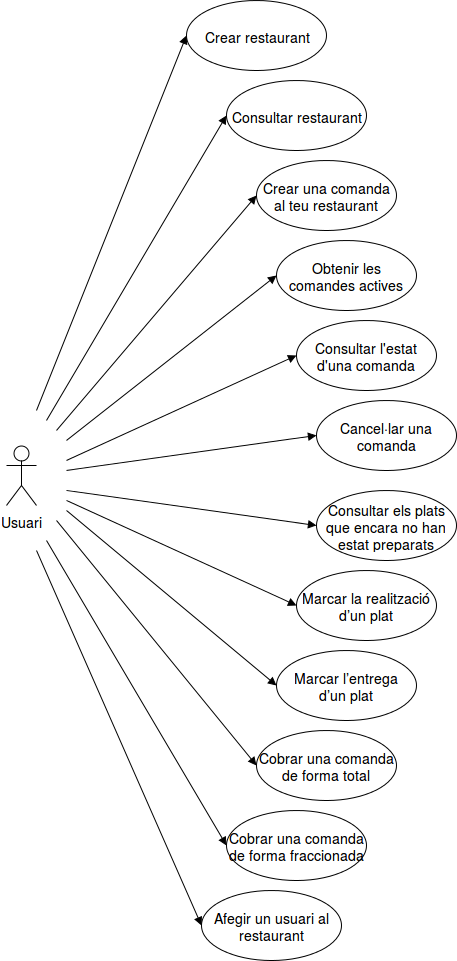
\includegraphics[scale=0.6]{Figures/casosUs_gestioEstabliment.png}
\caption{Diagrama de casos d'ús referent a la gestió de l'establiment}
\end{figure}

\begin{table}[!h]
\centering
\begin{tabular}{|l|L|l|}
\hline
\textbf{Cas d'ús}& \#6 & Crear restaurant \\ \hline
\textbf{Actor principal} & \multicolumn{2}{l|}{Usuari} \\ \hline
\textbf{Precondició} & \multicolumn{2}{M|}{L'usuari ha accedit a la pantalla principal de l'aplicació.} \\ \hline
\textbf{Trigger} & \multicolumn{2}{M|}{L'usuari vol crear un restaurant amb tots els seus detalls i informació.} \\ \hline
\multicolumn{3}{|T|}{\textbf{Escenari principal d'èxit}} \\ \hline
\multicolumn{3}{|T|}{1. L'usuari clica sobre el \textit{Navigational drawer} amb l'objectiu de fer-lo desplegar.}\\
\multicolumn{3}{|T|}{2. El sistema desplega el menú lateral.}\\
\multicolumn{3}{|T|}{3. L'usuari clica sobre la pestanya anomenada \textit{Create restaurant} situada a la part superior del menú lateral.}\\
\multicolumn{3}{|T|}{4. El sistema redirigeix a l'usuari a la pantalla de creació del restaurant.}\\
\multicolumn{3}{|T|}{5. L'usuari completa tots els camps disponibles (nom, descripció, localització, telèfon de contacte, pàgina web i nombre de taules) i després acciona el botó de següent situat a la part inferior-dreta.}\\
\multicolumn{3}{|T|}{6. El sistema redirigeix a l'usuari a la pantalla de creació d'horaris d'apertura.}\\
\multicolumn{3}{|T|}{7. L'usuari completa l'horari d'apertura i de clausura dels set dies de la setmana, i acciona el botó de següent situat a la part inferior-dreta.}\\
\multicolumn{3}{|T|}{8. El sistema redirigeix a l'usuari a la pantalla de creació de plats i menús.}\\
\multicolumn{3}{|T|}{9. L'usuari crea plats i menús accionant sobre l'opció especifica del menú desplegable de la part inferior-dreta especificant el nom, la descripció i el preu, i el conjunt de plats en cas del menú. Un cop finalitzat, l'usuari acciona el botó de la part superior-dreta per finalitzar la creació del restaurant. }\\
\multicolumn{3}{|T|}{10. El sistema redirigeix a l'usuari a la pantalla principal de l'aplicació, ja amb el restaurant creat i vinculat amb l'usuari actual.}\\
\hline
\multicolumn{3}{|T|}{\textbf{Extensions}} \\ \hline
\multicolumn{3}{|T|}{5.a L'usuari cancel·la els canvis en la informació bàsica} \\
\multicolumn{3}{|T|}{\tab5.a.1 L'usuari clica sobre la marxa enrere de la barra superior.} \\
\multicolumn{3}{|T|}{\tab5.a.2 El sistema redirigeix a l'usuari a la pantalla principal de l'aplicació sense cap canvi emmagatzemat.} \\
\multicolumn{3}{|T|}{7.a L'usuari cancel·la els canvis en l'apertura del restaurant} \\
\multicolumn{3}{|T|}{\tab7.a.1 L'usuari clica sobre la marxa enrere de la barra superior.} \\
\multicolumn{3}{|T|}{\tab7.a.2 El sistema redirigeix a l'usuari a la pantalla d'informació bàsica del restaurant sense cap canvi emmagatzemat.} \\
\multicolumn{3}{|T|}{9.a L'usuari cancel·la els canvis en la creació dels plats i menús} \\
\multicolumn{3}{|T|}{\tab9.a.1 L'usuari clica sobre la marxa enrere de la barra superior.} \\
\multicolumn{3}{|T|}{\tab9.a.2 El sistema redirigeix a l'usuari a la pantalla d'horaris d'apertura del restaurant sense cap canvi emmagatzemat.} \\
\hline
\end{tabular}
\label{}
\caption{Cas d'ús \textit{Crear restaurant}}
\end{table}

\begin{table}[!h]
\centering
\begin{tabular}{|l|L|l|}
\hline
\textbf{Cas d'ús}& \#7 & Consultar restaurant \\ \hline
\textbf{Actor principal} & \multicolumn{2}{l|}{Usuari} \\ \hline
\textbf{Precondició} & \multicolumn{2}{M|}{L'usuari ha accedit a la pantalla principal de l'aplicació.} \\ \hline
\textbf{Trigger} & \multicolumn{2}{M|}{L'usuari vol consultar el seu restaurant.} \\ \hline
\multicolumn{3}{|T|}{\textbf{Escenari principal d'èxit}} \\ \hline
\multicolumn{3}{|T|}{1. L'usuari clica sobre el \textit{Navigational drawer} amb l'objectiu de fer-lo desplegar.}\\
\multicolumn{3}{|T|}{2. El sistema desplega el menú lateral.}\\
\multicolumn{3}{|T|}{3. L'usuari clica sobre la pestanya anomenada \textit{See restaurant} del menú lateral.}\\
\multicolumn{3}{|T|}{4. El sistema redirigeix a l'usuari a la pantalla de vista del restaurant.}\\
\hline
\end{tabular}
\label{}
\caption{Cas d'ús \textit{Consultar restaurant}}
\end{table}

\begin{table}[!h]
\centering
\begin{tabular}{|l|L|l|}
\hline
\textbf{Cas d'ús}& \#8 & Crear una comanda al teu restaurant \\ \hline
\textbf{Actor principal} & \multicolumn{2}{l|}{Usuari} \\ \hline
\textbf{Precondició} & \multicolumn{2}{M|}{L'usuari ha accedit a la pantalla de comandes actives.} \\ \hline
\textbf{Trigger} & \multicolumn{2}{M|}{L'usuari vol crear una comanda al seu restaurant amb tots els detalls que la caracteritzen.} \\ \hline
\multicolumn{3}{|T|}{\textbf{Escenari principal d'èxit}} \\ \hline
\multicolumn{3}{|T|}{1. L'usuari clica sobre el botó rodó de la part de la part inferior de la pantalla.}\\
\multicolumn{3}{|T|}{2. El sistema mostra un desplegable amb un petit formulari per introduir la taula a on es realitza la comanda.}\\
\multicolumn{3}{|T|}{3. L'usuari escriu el número de taula a on es realitza la comanda i prem \textit{Acceptar}.}\\
\multicolumn{3}{|T|}{4. El sistema redirigeix a l'usuari a la pantalla de creació de comanda.}\\
\multicolumn{3}{|T|}{5. L'usuari selecciona els plats i menús que desitja el client prement el botó de \textit{+} de cada un dels ítems de la carta. En cas que estiguem parlant d'un menú, s'haurà de seleccionar quins plats es vol del menú determinat. Un cop tot completat, l'usuari clica sobre el botó de la part superior-dreta per finalitzar la creació de la comanda.}\\
\multicolumn{3}{|T|}{6. El sistema redirigeix a l'usuari a la pantalla de comandes actives amb la nova comanda emmagatzemada.}\\
\hline
\multicolumn{3}{|T|}{\textbf{Extensions}} \\ \hline
\multicolumn{3}{|T|}{5.a L'usuari cancel·la els canvis} \\
\multicolumn{3}{|T|}{\tab5.a.1 L'usuari clica sobre la marxa enrere de la barra superior.} \\
\multicolumn{3}{|T|}{\tab5.a.2 El sistema redirigeix a l'usuari a la pantalla de comandes actives sense cap canvi emmagatzemat.} \\\hline
\end{tabular}
\label{}
\caption{Cas d'ús \textit{Crear una comanda al teu restaurant}}
\end{table}

\begin{table}[!h]
\centering
\begin{tabular}{|l|L|l|}
\hline
\textbf{Cas d'ús}& \#9 & Obtenir les comandes actives \\ \hline
\textbf{Actor principal} & \multicolumn{2}{l|}{Usuari} \\ \hline
\textbf{Precondició} & \multicolumn{2}{M|}{L'usuari ha accedit a la pantalla principal de l'aplicació.} \\ \hline
\textbf{Trigger} & \multicolumn{2}{M|}{L'usuari vol consultar les comandes actives.} \\ \hline
\multicolumn{3}{|T|}{\textbf{Escenari principal d'èxit}} \\ \hline
\multicolumn{3}{|T|}{1. L'usuari clica sobre el \textit{Navigational drawer} amb l'objectiu de fer-lo desplegar.}\\
\multicolumn{3}{|T|}{2. El sistema desplega el menú lateral.}\\
\multicolumn{3}{|T|}{3. L'usuari clica sobre la pestanya anomenada \textit{Active orders} del menú lateral.}\\
\multicolumn{3}{|T|}{4. El sistema redirigeix a l'usuari a la pantalla de comandes actives del restaurant.}\\
\hline
\end{tabular}
\label{}
\caption{Cas d'ús \textit{Obtenir les comandes actives}}
\end{table}

\begin{table}[!h]
\centering
\begin{tabular}{|l|L|l|}
\hline
\textbf{Cas d'ús}& \#10 & Consultar l'estat d'una comanda \\ \hline
\textbf{Actor principal} & \multicolumn{2}{l|}{Usuari} \\ \hline
\textbf{Precondició} & \multicolumn{2}{M|}{L'usuari ha accedit a la pantalla de comandes actives.} \\ \hline
\textbf{Trigger} & \multicolumn{2}{M|}{L'usuari vol consultar l'estat d'una comanda.} \\ \hline
\multicolumn{3}{|T|}{\textbf{Escenari principal d'èxit}} \\ \hline
\multicolumn{3}{|T|}{1. L'usuari clica sobre alguna de les comandes que disposa en el llistat.}\\
\multicolumn{3}{|T|}{2. El sistema redirigeix a l'usuari a la vista de detall de la comanda.}\\
\hline
\end{tabular}
\label{}
\caption{Cas d'ús \textit{Consultar l'estat d'una comanda}}
\end{table}

\begin{table}[!h]
\centering
\begin{tabular}{|l|L|l|}
\hline
\textbf{Cas d'ús}& \#11 & Cancel·lar una comanda \\ \hline
\textbf{Actor principal} & \multicolumn{2}{l|}{L'usuari ha accedit a la pantalla de detall de la comanda.} \\ \hline
\textbf{Trigger} & \multicolumn{2}{M|}{L'usuari vol cancel·lar una comanda.} \\ \hline
\multicolumn{3}{|T|}{\textbf{Escenari principal d'èxit}} \\ \hline
\multicolumn{3}{|T|}{1. L'usuari clica sobre la icona de la cantonada esquerra de la barra superior.}\\
\multicolumn{3}{|T|}{2. El sistema mostra a l'usuari un desplegable amb l'opció de cancel·lar la comanda.}\\
\multicolumn{3}{|T|}{3. L'usuari clica sobre l'opció de cancel·lar comanda}\\
\multicolumn{3}{|T|}{4. El sistema redirigeix a l'usuari a la pantalla principal de l'aplicació, ja amb la comanda cancel·lada}\\
\hline
\end{tabular}
\label{}
\caption{Cas d'ús \textit{Cancel·lar una comanda}}
\end{table}

\begin{table}[!h]
\centering
\begin{tabular}{|l|L|l|}
\hline
\textbf{Cas d'ús}& \#12 & Consultar els plats que encara no han estat preparats \\ \hline
\textbf{Actor principal} & \multicolumn{2}{l|}{Usuari} \\ \hline
\textbf{Precondició} & \multicolumn{2}{M|}{L'usuari ha accedit a la pantalla principal de l'aplicació.} \\ \hline
\textbf{Trigger} & \multicolumn{2}{M|}{L'usuari vol consultar els plats que encara no han estat preparats.} \\ \hline
\multicolumn{3}{|T|}{\textbf{Escenari principal d'èxit}} \\ \hline
\multicolumn{3}{|T|}{1. L'usuari clica sobre el \textit{Navigational drawer} amb l'objectiu de fer-lo desplegar.}\\
\multicolumn{3}{|T|}{2. El sistema desplega el menú lateral.}\\
\multicolumn{3}{|T|}{3. L'usuari clica sobre la pestanya anomenada \textit{Kitchen} del menú lateral.}\\
\multicolumn{3}{|T|}{4. El sistema redirigeix a l'usuari a la pantalla de cuina.}\\
\hline
\end{tabular}
\label{}
\caption{Cas d'ús \textit{Consultar els plats que encara no han estat preparats}}
\end{table}

\begin{table}[!h]
\centering
\begin{tabular}{|l|L|l|}
\hline
\textbf{Cas d'ús}& \#13 & Marcar la realització d'un plat \\ \hline
\textbf{Actor principal} & \multicolumn{2}{l|}{Usuari} \\ \hline
\textbf{Precondició} & \multicolumn{2}{M|}{L'usuari ha accedit a la pantalla de cuina.} \\ \hline
\textbf{Trigger} & \multicolumn{2}{M|}{L'usuari vol marcar la realització d'un plat no preparat.} \\ \hline
\multicolumn{3}{|T|}{\textbf{Escenari principal d'èxit}} \\ \hline
\multicolumn{3}{|T|}{1. L'usuari selecciona l'ítem que ja ha preparat i confirma la seva elecció prement \textit{Acceptar}.}\\
\multicolumn{3}{|T|}{2. El sistema emmagatzema el canvi i elimina l'ítem del llistat.}\\
\hline
\end{tabular}
\label{}
\caption{Cas d'ús \textit{Marcar la realització d'un plat}}
\end{table}

\begin{table}[!h]
\centering
\begin{tabular}{|l|L|l|}
\hline
\textbf{Cas d'ús}& \#14 & Marcar l'entrega d'un plat \\ \hline
\textbf{Actor principal} & \multicolumn{2}{l|}{Usuari} \\ \hline
\textbf{Precondició} & \multicolumn{2}{M|}{L'usuari ha accedit a la pantalla de detall de la comanda.} \\ \hline
\textbf{Trigger} & \multicolumn{2}{M|}{L'usuari vol marcar l'entrega d'un plat.} \\ \hline
\multicolumn{3}{|T|}{\textbf{Escenari principal d'èxit}} \\ \hline
\multicolumn{3}{|T|}{1. L'usuari selecciona el botó rodó vinculat amb l'ítem desitjat i que vol marcar com a entregat.}\\
\multicolumn{3}{|T|}{2. El sistema emmagatzema el canvi.}\\
\hline
\end{tabular}
\label{}
\caption{Cas d'ús \textit{Marcar l'entrega d'un plat}}
\end{table}

\begin{table}[!h]
\centering
\begin{tabular}{|l|L|l|}
\hline
\textbf{Cas d'ús}& \#15 & Cobrar una comanda de forma total \\ \hline
\textbf{Actor principal} & \multicolumn{2}{l|}{Usuari} \\ \hline
\textbf{Precondició} & \multicolumn{2}{M|}{L'usuari ha accedit a la pantalla de detall de la comanda.} \\ \hline
\textbf{Trigger} & \multicolumn{2}{M|}{L'usuari vol cobrar una comanda de forma total.} \\ \hline
\multicolumn{3}{|T|}{\textbf{Escenari principal d'èxit}} \\ \hline
\multicolumn{3}{|T|}{1. L'usuari clica al botó rodó de la part inferior-dreta de la pantalla.}\\
\multicolumn{3}{|T|}{2. El sistema mostra un diàleg en el qual et permet elegir fer el cobrament parcialment o no.}\\
\multicolumn{3}{|T|}{3. L'usuari clica sobre \textit{All}.}\\
\multicolumn{3}{|T|}{4. El sistema tanca el diàleg i en mostra un altre confirmant la recol·lecta del total de la comanda.}\\
\multicolumn{3}{|T|}{5. L'usuari clica sobre \textit{Yes}.}\\
\multicolumn{3}{|T|}{6. El sistema tanca el diàleg i emmagatzema les dades marcant com a cobrada la comanda corresponent.}\\
\hline
\end{tabular}
\label{}
\caption{Cas d'ús \textit{Cobrar una comanda de forma total}}
\end{table}

\begin{table}[!h]
\centering
\begin{tabular}{|l|L|l|}
\hline
\textbf{Cas d'ús}& \#16 & Cobrar una comanda de forma fraccionada \\ \hline
\textbf{Actor principal} & \multicolumn{2}{l|}{Usuari} \\ \hline
\textbf{Precondició} & \multicolumn{2}{M|}{L'usuari ha accedit a la pantalla de detall de la comanda.} \\ \hline
\textbf{Trigger} & \multicolumn{2}{M|}{L'usuari vol cobrar una comanda de forma fraccionada.} \\ \hline
\multicolumn{3}{|T|}{\textbf{Escenari principal d'èxit}} \\ \hline
\multicolumn{3}{|T|}{1. L'usuari clica al botó rodó de la part inferior-dreta de la pantalla.}\\
\multicolumn{3}{|T|}{2. El sistema mostra un diàleg en el qual et permet elegir fer el cobrament parcialment o no.}\\
\multicolumn{3}{|T|}{3. L'usuari clica sobre \textit{In groups}.}\\
\multicolumn{3}{|T|}{4. El sistema tanca el diàleg i mostra tots els ítems que encara no han estat cobrats de la comanda.}\\
\multicolumn{3}{|T|}{5. L'usuari selecciona els ítems que vol cobrar i clica sobre el botó rodó de la part inferior de la pantalla.}\\
\multicolumn{3}{|T|}{6. El sistema mostra un diàleg confirmant la recol·lecta dels elements seleccionats dins la comanda.}\\
\multicolumn{3}{|T|}{7. L'usuari clica sobre \textit{Yes}.}\\
\multicolumn{3}{|T|}{8. El sistema tanca el diàleg i emmagatzema les dades marcant com a cobrats els plats corresponents.}\\
\hline
\end{tabular}
\label{}
\caption{Cas d'ús \textit{Cobrar una comanda de forma fraccionada}}
\end{table}

\begin{table}[!h]
\centering
\begin{tabular}{|l|L|l|}
\hline
\textbf{Cas d'ús}& \#17 & Afegir un usuari al restaurant \\ \hline
\textbf{Actor principal} & \multicolumn{2}{l|}{Usuari} \\ \hline
\textbf{Precondició} & \multicolumn{2}{M|}{L'usuari ha accedit a la pantalla de detall del restaurant.} \\ \hline
\textbf{Trigger} & \multicolumn{2}{M|}{L'usuari vol afegir un usuari dins de l'equip del restaurant.} \\ \hline
\multicolumn{3}{|T|}{\textbf{Escenari principal d'èxit}} \\ \hline
\multicolumn{3}{|T|}{1. L'usuari clica sobre el botó rodó de la barra superior.}\\
\multicolumn{3}{|T|}{2. El sistema mostra un diàleg amb un petit formulari per introduir l'adreça de correu electrònic de l'usuari a afegir.}\\
\multicolumn{3}{|T|}{3. L'usuari escriu l'adreça de correu electrònic de l'usuari a afegir.}\\
\multicolumn{3}{|T|}{4. El sistema emmagatzema la informació i tanca el diàleg.}\\
\hline
\multicolumn{3}{|T|}{\textbf{Extensions}} \\ \hline
\multicolumn{3}{|T|}{3.a L'usuari no existeix} \\
\multicolumn{3}{|T|}{\tab3.a.1 L'usuari introdueix una adreça electrònica no registrada a la base de dades de la plataforma.} \\
\multicolumn{3}{|T|}{\tab3.a.2 El sistema reporta la incidència a l'usuari i tanca el diàleg sense cap canvi en la persistència de la plataforma.} \\
\multicolumn{3}{|T|}{3.b L'usuari ja pertany a un restaurant} \\
\multicolumn{3}{|T|}{\tab3.b.1 L'usuari introdueix una adreça electrònica pertanyent a un usuari que ja està vinculat a un restaurant.} \\
\multicolumn{3}{|T|}{\tab3.b.2 El sistema reporta la incidència a l'usuari i tanca el diàleg sense cap canvi en la persistència de la plataforma.} \\
\hline
\end{tabular}
\label{}
\caption{Cas d'ús \textit{Afegir un usuari al restaurant}}
\end{table}

\clearpage
\subsection{Anàlisi de l'establiment}
\begin{figure}[H]
\centering
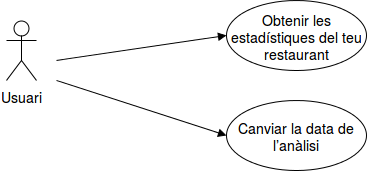
\includegraphics[scale=0.6]{Figures/casosUs_analisiEstabliment.png}
\caption{Diagrama de casos d'ús referent a l'anàlisi de l'establiment}
\end{figure}

\begin{table}[!h]
\centering
\begin{tabular}{|l|L|l|}
\hline
\textbf{Cas d'ús}& \#18 & Obtenir les estadístiques del teu restaurant  \\ \hline
\textbf{Actor principal} & \multicolumn{2}{l|}{Usuari} \\ \hline
\textbf{Precondició} & \multicolumn{2}{M|}{L'usuari ha accedit a la pantalla principal de l'aplicació.} \\ \hline
\textbf{Trigger} & \multicolumn{2}{M|}{L'usuari vol consultar les estadístiques del seu restaurant.} \\ \hline
\multicolumn{3}{|T|}{\textbf{Escenari principal d'èxit}} \\ \hline
\multicolumn{3}{|T|}{1. L'usuari clica sobre el \textit{Navigational drawer} amb l'objectiu de fer-lo desplegar.}\\
\multicolumn{3}{|T|}{2. El sistema desplega el menú lateral.}\\
\multicolumn{3}{|T|}{3. L'usuari clica sobre la pestanya anomenada \textit{Analytics} del menú lateral.}\\
\multicolumn{3}{|T|}{4. El sistema redirigeix a l'usuari a la pantalla d'estadístiques.}\\
\hline
\end{tabular}
\label{}
\caption{Cas d'ús \textit{Obtenir les estadístiques del teu restaurant}}
\end{table}

\begin{table}[!h]
\centering
\begin{tabular}{|l|L|l|}
\hline
\textbf{Cas d'ús}& \#19 & Canviar la data de l'anàlisi  \\ \hline
\textbf{Actor principal} & \multicolumn{2}{l|}{Usuari} \\ \hline
\textbf{Precondició} & \multicolumn{2}{M|}{L'usuari ha accedit a la pantalla d'estadístiques.} \\ \hline
\textbf{Trigger} & \multicolumn{2}{M|}{L'usuari vol canviar la data de visualització per analitzar les estadístiques d'un altre període.} \\ \hline
\multicolumn{3}{|T|}{\textbf{Escenari principal d'èxit}} \\ \hline
\multicolumn{3}{|T|}{1. L'usuari clica sobre el botó amb icona de calendari situat a la barra superior.}\\
\multicolumn{3}{|T|}{2. El sistema mostra un diàleg amb un calendari per seleccionar una data.}\\ 
\multicolumn{3}{|T|}{3. L'usuari selecciona un dia del calendari i prem \textit{Acceptar}.}\\ 
\multicolumn{3}{|T|}{4. El sistema refresca la vista amb la nova data seleccionada i tanca el diàleg.}\\ 
\hline
\end{tabular}
\label{}
\caption{Cas d'ús \textit{Canviar la data de l'anàlisi}}
\end{table}

\clearpage
\subsection{Interacció del client}
\begin{figure}[H]
\centering
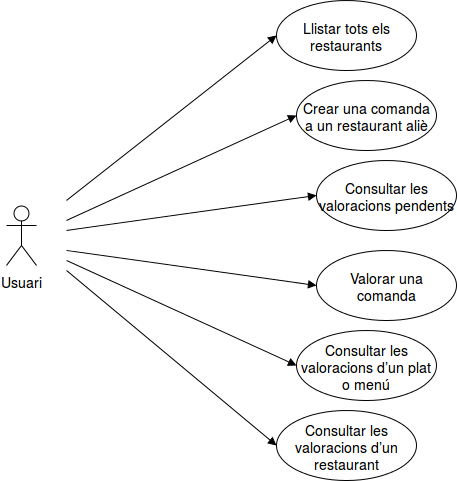
\includegraphics[scale=0.6]{Figures/casosUs_interaccioClient.png}
\caption{Diagrama de casos d'ús referent a la interacció del client}
\end{figure}

\begin{table}[!h]
\centering
\begin{tabular}{|l|L|l|}
\hline
\textbf{Cas d'ús}& \#20 & Llistar tots els restaurants  \\ \hline
\textbf{Actor principal} & \multicolumn{2}{l|}{Usuari} \\ \hline
\textbf{Precondició} & \multicolumn{2}{M|}{L'usuari ha accedit a la pantalla principal de l'aplicació.} \\ \hline
\textbf{Trigger} & \multicolumn{2}{M|}{L'usuari vol consultar els restaurants emmagatzemats dins la plataforma.} \\ \hline
\multicolumn{3}{|T|}{\textbf{Escenari principal d'èxit}} \\ \hline
\multicolumn{3}{|T|}{1. L'usuari clica sobre el \textit{Navigational drawer} amb l'objectiu de fer-lo desplegar.}\\
\multicolumn{3}{|T|}{2. El sistema desplega el menú lateral.}\\
\multicolumn{3}{|T|}{3. L'usuari clica sobre la pestanya anomenada \textit{List restaurants} del menú lateral.}\\
\multicolumn{3}{|T|}{4. El sistema redirigeix a l'usuari a la pantalla referent al llistat de restaurants.}\\
\hline
\end{tabular}
\label{}
\caption{Cas d'ús \textit{Llistar tots els restaurants}}
\end{table}

\begin{table}[!h]
\centering
\begin{tabular}{|l|L|l|}
\hline
\textbf{Cas d'ús}& \#21 & Crear una comanda a un restaurant aliè  \\ \hline
\textbf{Actor principal} & \multicolumn{2}{l|}{Usuari} \\ \hline
\textbf{Precondició} & \multicolumn{2}{M|}{L'usuari ha accedit a la pantalla referent al llistat dels restaurants.} \\ \hline
\textbf{Trigger} & \multicolumn{2}{M|}{L'usuari vol crear una comanda a un restaurant aliè.} \\ \hline
\multicolumn{3}{|T|}{\textbf{Escenari principal d'èxit}} \\ \hline
\multicolumn{3}{|T|}{1. L'usuari selecciona algun dels restaurants del llistat.}\\
\multicolumn{3}{|T|}{2. El sistema redirigeix a l'usuari a la pantalla de vista d'un restaurant.}\\ 
\multicolumn{3}{|T|}{3. L'usuari clica sobre el botó rodó de la barra superior.}\\ 
\multicolumn{3}{|T|}{4. El sistema mostra un desplegable amb un petit formulari per introduir la taula a on es realitza la comanda.}\\
\multicolumn{3}{|T|}{5. L'usuari escriu el número de taula a on es realitza la comanda i prem \textit{Acceptar}.}\\
\multicolumn{3}{|T|}{6. El sistema redirigeix a l'usuari a la pantalla de creació de comanda.}\\
\multicolumn{3}{|T|}{7. L'usuari selecciona els plats i menús que desitja prement el botó de \textit{+} de cada un dels ítems de la carta. En cas que estiguem parlant d'un menú, s'haurà de seleccionar quins plats es vol del menú determinat. Un cop tot completat, l'usuari clica sobre el botó de la part superior-dreta per finalitzar la creació de la comanda.}\\
\multicolumn{3}{|T|}{8. El sistema redirigeix a l'usuari a la pantalla de visualització del restaurant amb la nova comanda emmagatzemada.}\\
\hline
\multicolumn{3}{|T|}{\textbf{Extensions}} \\ \hline
\multicolumn{3}{|T|}{7.a L'usuari cancel·la els canvis} \\
\multicolumn{3}{|T|}{\tab7.a.1 L'usuari clica sobre la marxa enrere de la barra superior.} \\
\multicolumn{3}{|T|}{\tab7.a.2 El sistema redirigeix a l'usuari a la pantalla de visualització del restaurant sense cap canvi emmagatzemat.} \\\hline
\end{tabular}
\label{}
\caption{Cas d'ús \textit{Crear una comanda a un restaurant aliè}}
\end{table}

\begin{table}[!h]
\centering
\begin{tabular}{|l|L|l|}
\hline
\textbf{Cas d'ús}& \#22 & Consultar les valoracions pendents  \\ \hline
\textbf{Actor principal} & \multicolumn{2}{l|}{Usuari} \\ \hline
\textbf{Precondició} & \multicolumn{2}{M|}{L'usuari ha accedit a la pantalla principal de l'aplicació.} \\ \hline
\textbf{Trigger} & \multicolumn{2}{M|}{L'usuari vol consultar les seves valoracions pendents.} \\ \hline
\multicolumn{3}{|T|}{\textbf{Escenari principal d'èxit}} \\ \hline
\multicolumn{3}{|T|}{1. L'usuari clica sobre el \textit{Navigational drawer} amb l'objectiu de fer-lo desplegar.}\\
\multicolumn{3}{|T|}{2. El sistema desplega el menú lateral.}\\
\multicolumn{3}{|T|}{3. L'usuari clica sobre la pestanya anomenada \textit{Pending reviews} del menú lateral.}\\
\multicolumn{3}{|T|}{4. El sistema redirigeix a l'usuari a la pantalla de valoracions pendents.}\\
\hline
\end{tabular}
\label{}
\caption{Cas d'ús \textit{Consultar les valoracions pendents}}
\end{table}

\begin{table}[!h]
\centering
\begin{tabular}{|l|L|l|}
\hline
\textbf{Cas d'ús}& \#23 & Valorar una comanda  \\ \hline
\textbf{Actor principal} & \multicolumn{2}{l|}{Usuari} \\ \hline
\textbf{Precondició} & \multicolumn{2}{M|}{L'usuari ha accedit a la pantalla de valoracions pendents.} \\ \hline
\textbf{Trigger} & \multicolumn{2}{M|}{L'usuari vol valorar una de les comandes que té pendents per valorar.} \\ \hline
\multicolumn{3}{|T|}{\textbf{Escenari principal d'èxit}} \\ \hline
\multicolumn{3}{|T|}{1. Selecciona una de les comandes que té per valorar.}\\
\multicolumn{3}{|T|}{2. El sistema redirigeix a l'usuari a la vista de valoració.}\\ 
\multicolumn{3}{|T|}{3. L'usuari puntua amb una puntuació fins a 5 estrelles cada un dels plats que formen la comanda i afegeix un comentari opcional que complementa la valoració. A més a més, també valora el restaurant de forma global amb una puntuació i un comentari opcional. Un cop finalitzat acciona el botó de la part inferior de la pantalla.}\\ 
\multicolumn{3}{|T|}{4. El sistema emmagatzema les dades introduïdes i redirigeix a l'usuari a la pantalla de valoracions pendents.}\\ 
\hline
\multicolumn{3}{|T|}{\textbf{Extensions}} \\ \hline
\multicolumn{3}{|T|}{3.a L'usuari cancel·la els canvis} \\
\multicolumn{3}{|T|}{\tab3.a.1 L'usuari clica sobre la marxa enrere de la barra superior.} \\
\multicolumn{3}{|T|}{\tab3.a.2 El sistema redirigeix a l'usuari a la pantalla de valoracions pendents sense cap canvi emmagatzemat.} \\\hline
\end{tabular}
\label{}
\caption{Cas d'ús \textit{Valorar una comanda}}
\end{table}

\begin{table}[!h]
\centering
\begin{tabular}{|l|L|l|}
\hline
\textbf{Cas d'ús}& \#24 & Consultar les valoracions d'un plat o menú  \\ \hline
\textbf{Actor principal} & \multicolumn{2}{l|}{Usuari} \\ \hline
\textbf{Precondició} & \multicolumn{2}{M|}{L'usuari ha accedit a la pantalla referent al llistat dels restaurants.} \\ \hline
\textbf{Trigger} & \multicolumn{2}{M|}{L'usuari vol consultar les valoracions d'un plat o menú d'un restaurant aliè.} \\ \hline
\multicolumn{3}{|T|}{\textbf{Escenari principal d'èxit}} \\ \hline
\multicolumn{3}{|T|}{1. L'usuari selecciona algun dels restaurants del llistat.}\\
\multicolumn{3}{|T|}{2. El sistema redirigeix a l'usuari a la pantalla de vista d'un restaurant.}\\ 
\multicolumn{3}{|T|}{3. L'usuari manté clicat sobre un dels plats o menús del restaurant.}\\
\multicolumn{3}{|T|}{4. El sistema mostra un diàleg amb estadístiques i informació bàsica sobre l'ítem seleccionat.}\\
\multicolumn{3}{|T|}{5. L'usuari clica sobre el botó del diàleg amb títol \textit{Reviews}.}\\
\multicolumn{3}{|T|}{6. El sistema redirigeix a l'usuari a la pantalla de valoracions de l'ítem seleccionat.}\\
\hline
\end{tabular}
\label{}
\caption{Cas d'ús \textit{Consultar les valoracions d'un plat o menú.}}
\end{table}

\begin{table}[!h]
\centering
\begin{tabular}{|l|L|l|}
\hline
\textbf{Cas d'ús}& \#25 & Consultar les valoracions d'un restaurant  \\ \hline
\textbf{Actor principal} & \multicolumn{2}{l|}{Usuari} \\ \hline
\textbf{Precondició} & \multicolumn{2}{M|}{L'usuari ha accedit a la pantalla referent al llistat dels restaurants.} \\ \hline
\textbf{Trigger} & \multicolumn{2}{M|}{L'usuari vol consultar les valoracions d'un restaurant.} \\ \hline
\multicolumn{3}{|T|}{\textbf{Escenari principal d'èxit}} \\ \hline
\multicolumn{3}{|T|}{1. L'usuari selecciona algun dels restaurants del llistat.}\\
\multicolumn{3}{|T|}{2. El sistema redirigeix a l'usuari a la pantalla de vista d'un restaurant.}\\ 
\multicolumn{3}{|T|}{3. L'usuari clica sobre la icona de la cantonada esquerra de la barra superior.}\\
\multicolumn{3}{|T|}{4. El sistema mostra a l'usuari un desplegable amb l'opció de consultar les valoracions sobre el restaurant.}\\
\multicolumn{3}{|T|}{5. L'usuari clica sobre l'opció de consultar les valoracions sobre el restaurant.}\\
\multicolumn{3}{|T|}{6. El sistema redirigeix a l'usuari a la pantalla de valoracions del restaurant seleccionat.}\\
\hline
\end{tabular}
\label{}
\caption{Cas d'ús \textit{Consultar les valoracions d'un restaurant}}
\end{table}
% Chapter Template

\chapter{Especificació} % Main chapter title

\label{Chapter5} % Change X to a consecutive number; for referencing this chapter elsewhere, use \ref{ChapterX}

Després d'haver explicat l'origen de \textit{Wisebite}, haver estudiat les solucions actuals del mercat i suggerit una de millor i haver analitzat els requisits i les funcionalitats del sistema, cal especificar els models que representaran les entitats que formaran el projecte. En primera instància, es mostrarà l'esquema conceptual que defineix el treball i s'explicarà cada una de les entitats que l'engloben. Per altra banda, s'analitzarà l'esquema de comportament que interacciona entre l'usuari i el sistema.

%----------------------------------------------------------------------------------------
%	SECTION 1
%----------------------------------------------------------------------------------------

\section{Esquema conceptual}

L'esquema conceptual d'un sistema és la representació gràfica dels models que caracteritzen aquest. En Enginyeria del Software això és conegut com un diagrama de classes\cite{diagramaclases}. Primerament, s'expressarà en format UML i posteriorment s'explicarà textualment.

\begin{figure}[!h]
\centering
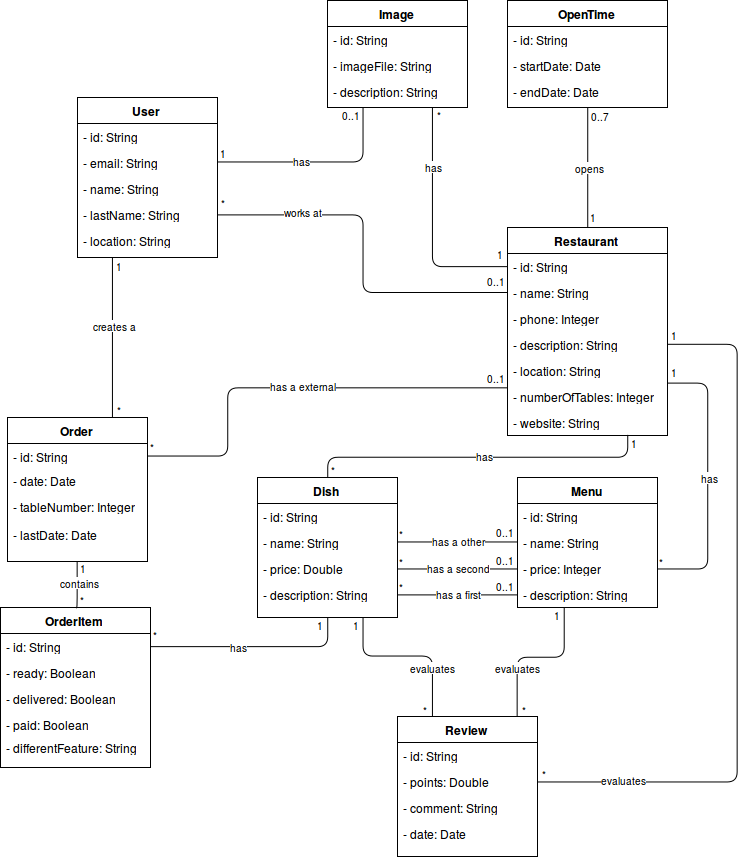
\includegraphics[scale=0.5]{Figures/diagrama_clases.png}
\caption{Diagrama de classes}
\end{figure}

%----------------------------------------------------------------------------------------
%	SECTION 2
%----------------------------------------------------------------------------------------

\clearpage
\section{Esquema del comportament}

TODO: Redactar
% Chapter Template

\chapter{Disseny} % Main chapter title

\label{Chapter6} % Change X to a consecutive number; for referencing this chapter elsewhere, use \ref{ChapterX}

Després d'haver mencionat, de forma molt específica, com és l'aplicació tant en requisits com en objectius, hem de veure com està construïda internament, és a dir, quin tipus d'arquitectura tècnica segueix, quin disseny de base de dades s'ha establert, com s'ha dissenyat el software implementat i amb quins patrons s'ha construït i finalment com s'ha definit la interfície de l'usuari.

%----------------------------------------------------------------------------------------
% SECTION 1
%----------------------------------------------------------------------------------------

\section{Arquitectura del sistema}

Després d'haver explicat quin és l'abast i quins objectius té \textit{Wisebite}, es va prendre la decisió que el projecte esdevingués a una plataforma mòbil per a dispositius Android. La justificació d'aquest fet ve dividida en dos punts, primer el fet que sigui un mòbil i no pas una aplicació web, per exemple, i l'altre pel fet que només s'hagi implementat per Android i no pas per cap altra sistema operatiu d'aquest tipus.
\\\\
En primera instància, el motiu principal pel qual \textit{Wisebite} ha estat implementat i dissenyat per dispositius mòbils és el dinamisme que aporten i del qual no disposen els dispositius de sobretaula. El món de la restauració és un sector de moviment continu, tant per part de l'empleat com per part del client. Un treballador d'un bar o restaurant es mourà de forma contínua per l'establiment i un client no sol acudir al mateix restaurant sempre. En conseqüència, el fet que \textit{Wisebite} estigui disponible en telèfons mòbils o bé tauletes permet als usuaris d'aquesta plataforma interactuar amb ella des de qualsevol lloc i de forma més còmode interactuant amb la pantalla tàctil que disposa el terminal.
\\\\
Per altra banda, \textit{Wisebite} s'ha especialitzat en sistemes operatius Android i no pas en algun altre per un seguit de factors que es comenten a continuació.
\\\\
En primer lloc és important recordar un dels tres factors pels quals sistemes d'aquest tipus no han acabat d'introduir-se dins el sector: el factor econòmic. En el mercat dels dispositius mòbils és vist i reconegut que els dispositius Android, donat el gran número de terminals en els quals opera, són de preu més reduït que pas els sistemes iOS, implementats per Apple. Així doncs, és important oferir hardware barat als establiments que implantin \textit{Wisebite} per així reduir l'impacte econòmic que els pot ocasionar.
\\\\
En segon lloc, per què només per Android i no pas també per iOS? És cert que existeix un seguit de \textit{frameworks} que et permet desenvolupar aplicacions mòbils híbrides, és a dir, per a tots els sistemes operatius mòbils.
\\\\
La problemàtica principal d'aquest tipus de desenvolupament és el fet de no poder utilitzar tots els avantatges que et permet un sistema operatiu natiu en concret. Per exemple, si analitzem les aplicacions mòbils natives d'Android, veiem que tot el \textit{backend} de l'aplicació pot ser escrit en Java, C++ o bé Kotlin i el \textit{frontend} amb llenguatge d'etiquetes com és XML. En canvi, si es realitzes amb un dels \textit{frameworks} que ofereix el mercat s'escriuria en HTML, CSS i JavaScript, com si es tractés d'una pàgina web. Són maneres d'implementar aplicacions molt diferents, i per molt que aquests \textit{frameworks} ho vulguin simular al màxim no ho acaben d'aconseguir del tot. Així doncs, donat que un dels objectius clau que té \textit{Wisebite} és destacar per la seva interfície és molt millor implementar en llenguatge natiu donats els avantatges que t'ofereix.
\\\\
Per tant, donada aquesta justificació, l'aplicació correrà en dispositius exclusivament Android a partir de l'\textit{API 21} o versió \textit{5.0 Lollipop}, és a dir, en un 88.6\%\cite{androidOsAnalytics} dels dispositius de la marca de Google.
\\\\
Aquesta aplicació es comunica amb una base de dades no relacional (NoSQL) anomenada \textit{Firebase}. En apartats posteriors dins d'aquest mateix capítol s'explicarà com s'ha implementat l'esquema de dades dins d'aquest gestor, però abans en aquest apartat és important conèixer el perquè de l'elecció de \textit{Firebase} com a base de dades per a \textit{Wisebite}.
\\\\
\textit{Firebase} va ser comprada per Google el maig del 2016, fet que aporta serietat, fiabilitat i robustesa com a base de dades, és a dir, pertany a una de les institucions més importants dins el sector de la informàtica, per no dir el que més. Tot i així, el factor més important i pel qual es va decidir utilitzar aquesta base de dades no relacional és que la comunicació es realitza en temps real. Aquest aspecte és realment important sabent quina és la temàtica de l'aplicació. Es considera molt important aquest fet, ja que l'actualització automàtica de les dades sense necessitat de refresc manual facilita moltíssim la feina d'un cambrer o d'un cuiner a l'hora d'interactuar amb la plataforma. Així doncs, per aquest fet es va decidir implantar la base de dades dins de \textit{Firebase}.
\\\\
Per últim, l'aplicació emmagatzemarà les dades temporals en un \textit{SQLite} que actuarà de memòria cau dins de \textit{Wisebite}. La justificació de l'ús d'aquesta tecnologia ve donat pel fet que Android la utilitza de forma predefinida en les seves aplicacions natives.
\\\\
Per clarificar més el concepte i veure quina és la interacció de l'usuari amb \textit{Android}, \textit{Firebase} i \textit{SQLite}, es mostra a continuació una gràfica de l'arquitectura tècnica que s'ha decidit utilitzar a \textit{Wisebite}.
\begin{figure}[H]
\centering
\includegraphics[scale=0.25]{Figures/technical_architecture.png}
\caption{Arquitectura tècnica del sistema}
\end{figure}

%----------------------------------------------------------------------------------------
%	SECTION 2
%----------------------------------------------------------------------------------------

\section{Disseny de la base de dades}

Com s'ha comentat en l'apartat anterior, la base de dades de \textit{Wisebite} serà \textit{Firebase}. Aquesta base de dades funciona amb una estructura en forma d'arbre basant-se en el format JSON\cite{json}.
\\\\
Existeix un node pare o arrel anomenat \textit{wisebite-f7a53} del qual pengen tots els nodes restants. Per a tal de dissenyar una bona base de dades NoSQL de tipus clau-valor, com es \textit{Firebase}, és necessari tenir en compte un seguit de conceptes per seguir les bones pràctiques que les mateixes guies del gestor recomanen:
\begin{itemize}
\item El fet d'accedir a un node, fa que hagi de descarregar tot l'arbre del qual penja aquest node (amb tots els seus respectius fills). Per tant, la solució és disgregar els elements. Cal tenir cura en relacionar els components o nodes de la base de dades per poder-los processar correctament. Un bon mètode seria associar els elements via el seu identificador i no pas tot l'element.
\item Per realitzar relacions entre, per exemple, un restaurant i els usuaris als quals hi treballen podríem pensar en afegir un node fill per a cada usuari del restaurant. Això és ineficient en cas de tenir restaurants amb un gran nombre d'usuaris en ells. En conseqüència, la solució seria utilitzar índexs. Per a cada restaurant s'hauria de tenir un llistat d'usuaris on es representen els usuaris pertanyents a ell.
\end{itemize}

\noindent Llavors, en definitiva, el missatge més important és que cal tenir en compte que encara que \textit{Firebase} tingui una estructura en forma d'arbre, no s'ha de construir  esquema de profunditat molt gran, sinó millor crear un arbre amb la major amplada possible. Això farà més eficient les consultes a la base de dades.
\\\\
Després d'haver estudiat i entès quines són les bones pràctiques d'una base de dades no relacional de tipus clau-valor, s'ha dissenyat de tal manera que pengen nou nodes del node arrel, on allà s'emmagatzemen totes les instàncies d'aquella entitat. Cadascuna d'elles serà identificada a partir d'un identificador aleatori. Cadascun d'aquest nodes representen les nou entitats que han estat explicades en capítols anteriors. A continuació es mostra l'estructura de la base de dades en format JSON.

\clearpage
\begin{lstlisting}[language=json,firstnumber=1]
"wisebite-f7a53" : {
   "dish" : {
      "-KlPZWq5d4cFO6NJ0nc4" : {
         "description" : "Classic",
         "id" : "-KlPZWq5d4cFO6NJ0nc4",
         "name" : "Paella",
         "price" : 12,
         "reviews" : {
            "-KlyJ20Nr3OpnA0JLqk5" : true,
            "-Km3Q9par9GavvZHt-4L" : true,
            "-KmNrn1Gxu66N6tc5u32" : true
         }
      },
      ...
   },
   "image" : {
      "-KlPTsD8xjazZ8KceJ6E" : {
         "description" : "Profile photo",
         "id" : "-KlPTsD8xjazZ8KceJ6E",
         "imageFile" : "https://lh5.googleuser..."
      },
      ...
   },
   "menu" : {
      "-KlPeMorCJsXKHh024Ui" : {
         "description" : "nu",
         "id" : "-KlPeMorCJsXKHh024Ui"
         "mainDishes" : {
            "-KlPeLzph1_Sz7UGcnMc" : true
         },
         "name" : "menu",
         "otherDishes" : {
            "-KlPeLzrWp_u0Fx3bNPW" : true
         },
         "price" : 0.5,
         "secondaryDishes" : {
            "-KlPeLzrWp_u0Fx3bNPV" : true
         }
      },
      ...
   },
   "openTime" : {
      "-KlPY8bUts4c9domVn5d" : {
         "endDate" : {
            "date" : 29,
            "day" : 1,
            "hours" : 22,
            "minutes" : 0,
            "month" : 11,
            "seconds" : 0,
            "time" : -180000000,
            "timezoneOffset" : 0,
            "year" : 69
         },
         "id" : "-KlPY8bUts4c9domVn5d",
         "startDate" : {
            "date" : 29,
            "day" : 1,
            "hours" : 8,
            "minutes" : 0,
            "month" : 11,
            "seconds" : 0,
            "time" : -230400000,
            "timezoneOffset" : 0,
            "year" : 69
         }
       },
       ...
    },
   "order" : {
      "-KlZianOlkFpEkNFoiF7" : {
         "date" : {
            "date" : 1,
            "day" : 4,
            "hours" : 19,
            "minutes" : 35,
            "month" : 5,
            "seconds" : 58,
            "time" : 1496338558814,
            "timezoneOffset" : -120,
            "year" : 117
         },
         "id" : "-KlZianOlkFpEkNFoiF7",
         "lastDate" : {
            "date" : 1,
            "day" : 4,
            "hours" : 20,
            "minutes" : 37,
            "month" : 5,
            "seconds" : 53,
            "time" : 1496342273505,
            "timezoneOffset" : -120,
            "year" : 117
         },
         "orderItems" : {
            "-KlZian7yy0XgIJaGrCV" : true,
            "-KlZianHOSo5hbzboxWl" : true,
            "-KlZianKOdNMI1r06jnh" : true,
            "-KlZianMs7fEFfK3JJw7" : true
         },
         "tableNumber" : 9
      },
      ...
   },
   "orderItem" : {
      "-KlYSoFkb_Z7WmMsvNEy" : {
         "delivered" : false,
         "dishId" : "-KlPeMorCJsXKHh024Uh",
         "id" : "-KlYSoFkb_Z7WmMsvNEy",
         "menuId" : null,
         "paid" : true,
         "ready" : false
      },
      ...
   },
   "restaurant" : {
      "-KlPZWqHH5fEgUoCrGG5" : {
         "description" : "De tota la vida, de poble.",
         "dishes" : {
            "-KlPZWq-xR39JAJBEitN" : true,
            "-KlPZWq1k46MlYinfido" : true,
            "-KlPZWq3w_Zwu63am50p" : true,
            "-KlPZWq4OshyHXIufnFO" : true,
            "-KlPZWq5d4cFO6NJ0nc4" : true
         },
         "externalOrders" : {
            "-Kldj4NCYd-3ZN9H93Mh" : true,
            "-Kldk-C2wrOFKZmrtOPB" : true,
            "-Kldt2L6ZRJouCK75rzP" : true,
            "-KlyIcuVp1Lx3U7235PN" : true,
            "-Km3Q3B4u_Sq65WCv0bq" : true,
            "-KmNqGKk-EURs6mBnQNz" : true
         },
         "id" : "-KlPZWqHH5fEgUoCrGG5",
         "location" : "Sant Celoni",
         "menus" : {
            "-KlPZWq7lAVXkCYqe-Z9" : true,
            "-KlPZWqDD_UhNEVauAtt" : true,
            "-KlPZWqF14E1wMPYIHT6" : true
         },
         "name" : "Cerveseria Ceres",
         "numberOfTables" : 30,
         "openTimes" : {
            "-KlPY8bUts4c9domVn5d" : true,
            "-KlPY8bnpSPVrvXvEL6F" : true,
            "-KlPY8brvVHqL0KXCfEi" : true,
            "-KlPY8bz9HQijw46-WWE" : true,
            "-KlPY8c2YzO4D7yZ99zU" : true
         },
         "phone" : 666544283,
         "reviews" : {
            "-KlyJ20VJ77rNt1Yfg2y" : true,
            "-Km3Q9pddyCuqWYlCz-C" : true,
            "-KmNrn1L9CSgClEUHv_I" : true
         },
         "users" : {
            "alsumo95@gmail@com" : true
         },
         "website" : "ceres.com"
       },
       ...
    },
   "review" : {
      "-KltwNoh4fDoG7tIWZYx" : {
         "comment" : "Rico!",
         "date" : {
            "date" : 8,
            "day" : 4,
            "hours" : 9,
            "minutes" : 21,
            "month" : 5,
            "seconds" : 12,
            "time" : 1496906472539,
            "timezoneOffset" : -120,
            "year" : 117
         },
         "id" : "-KltwNoh4fDoG7tIWZYx",
         "points" : 4,
         "userId" : "alsumo95@gmail@com"
      },
      ...
   },
   "user" : {
      "alripol95@gmail@com" : {
         "email" : "alripol95@gmail.com",
         "id" : "alripol95@gmail@com",
         "imageId" : "-Km0MSeurykImTbkBPEl",
         "lastName" : "Ripol",
         "myOrders" : {
            "-Km0RcztK3XoafmEAx4P" : true
         },
         "myRestaurants" : {
            "-Km0Nbs9ioiglQBNVNvv" : true
         },
         "name" : "Albert",
         "ordersToReview" : {
            "-Km0RcztK3XoafmEAx4P" : true
         }
      },
      ...
   }
}
\end{lstlisting}

%----------------------------------------------------------------------------------------
%	SECTION 3
%----------------------------------------------------------------------------------------

\section{Disseny de software}

Durant el transcurs de la carrera, i en especial durant l'especialitat d'Enginyeria del Software, s'ha emfatitzat molt en el concepte que programar bé no és simplement que funcioni el programa implementat, sinó que segueixi uns patrons específics que et permeti tenir un codi fàcil d'entendre i re-usable, ja que al cap i a la fi el codi es llegeix més cops dels que s'escriu.
\\\\
És per això que en la implementació del projecte de \textit{Wisebite} s'ha seguit un conjunt de patrons de disseny de software anomenats patró repositori, patró servei, patró factoria i el més conegut anomenat MVC (Model-Vista-Controlador).

\subsection{Patrons de disseny}

S'ha utilitzat, com s'ha comentat anteriorment, quatre patrons de disseny durant la implementació de \textit{Wisebite}.

\begin{itemize}
\item \textbf{Patró repositori}: utilitzat per evitar l'accés directe a les dades, és a dir, des de la vista o més concretament en Android, des de l'\textit{Activity}. En aquest cas es permet desacoblar al màxim l'accés a \textit{Firebase}. Tota classe que serà traduïda en un objecte persistent en \textit{Firebase}, seguint el model de la base de dades mostrat al capítol anterior, ha d'implementar una interfície \textit{Entity}, i definirem una interfície \textit{Repository} parametritzada, sobre la qual caldrà implementar una classe \textit{RepositoryXXXX} que la implementi (on XXXX defineix l'objecte que emmagatzema el repositori), que seran instanciades i utilitzades amb els seus mètodes ja definits per accedir a \textit{Firebase}. Aquesta classe \textit{RepositoriXXXX} hereta d'una altre anomenada \textit{FirebaseRepository} per així afegir una capa més d'abstracció.
\\
\begin{figure}[h]
\centering
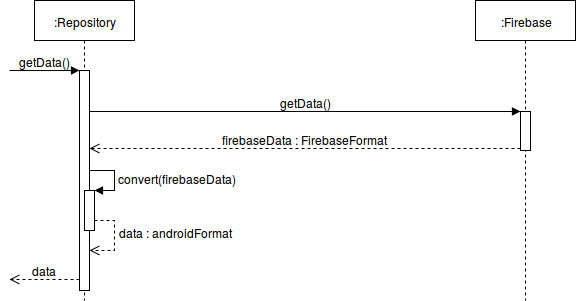
\includegraphics[scale=0.6]{Figures/patro_repositori.png}
\caption{Patró repositori}
\end{figure}

\item \textbf{Patró servei / injecció de dependència}: utilitzat per crear una capa d'abstracció sobre els dipòsits prèviament esmentats. En aquestes noves classes, les quals hereten d'una interfície anomenada \textit{Service}, ens permet executar la lògica del programa, sense necessitat d'accedir directament als repositoris. Aquests serveis contenen una instància única del repositori. Gràcies a la injecció de dependència podem realitzar tests de la lògica del programa sense haver de fer servir la base de dades real mitjançant \textit{mocking} dels repositoris. Malauradament, donat al factor temporal i que especificarem en capítols posteriors, no s'ha posat a la pràctica la utilitat dels tests. Tot i així, el codi del programa està ben preparat per poder afegir tests fàcilment.

\item \textbf{Patró factoria}: utilitzat per a la crida de serveis amb la creació d'un singleton anomenat \textit{ServiceFactory}. Permet abstreure la funcionalitat de creació del servei, permetent així evitar la creació repetitiva del servei a cada ús que se li dóna, fet que comportaria tenir moltes instàncies del mateix objecte repartides per l'execució de l'aplicació. Separa la instanciació del servei del seu ús. Permet que es faci injecció de dependències sense haver de saber l'estructura d'aquesta.

\item \textbf{MVC}: utilitzat per organitzar l'estructura de l'aplicació. En el cas de \textit{Wisebite} en tractar-se d'Android les vistes són les activities. D'altra banda els controladors s'han anomenat serveis.
\end{itemize}

\noindent Totes les classes Java comentades han estat adjuntades a l'apèndix \ref{AppendixA}.

%----------------------------------------------------------------------------------------
%	SECTION 4
%----------------------------------------------------------------------------------------

\section{Disseny de la interfície}

Com es va comentar en capítols anteriors, concretament en l'estudi de mercat, actualment existeixen aplicacions que en qüestió de funcionalitats s'assemblen o s'acosten al que busca \textit{Wisebite}, però la gran majoria d'aquestes no han dedicat molt temps en l'estudi de la gestió de la interfície d'usuari. En canvi, en aquest projecte s'ha dedicat més del temps mínim requerit per construir una interfície el millor possible per l'usuari.
\\\\
El primer factor que es va tenir en compte va ser l'ús de les directrius que marca el \textit{Material Design}, un estil de disseny d'interfícies que va néixer amb l'API 21 o versió 5.0 d'Android. Amb l'aparició d'aquest estil s'ha buscat en tot moment facilitar l'ús de les aplicacions a les persones que els hi costa més utilitzar aplicacions per a smartphones. Interfícies molt més intuïtives, de colors i formes característiques, amb més dinamisme en la navegació per la plataforma i, sobretot, un patró de disseny estable en tots els dispositius del mercat.
\\\\
\textit{Wisebite} ha decidit seguir aquest model, ja que és molt important no canviar molt la interfície a la qual està acostumat l'usuari amb altres aplicacions. Per aquest motiu doncs s'ha decidit seguir els dissenys preestablerts que facilita les guies de \textit{Material Design}.
\\\\
Durant la navegació de l'aplicació s'ha buscat tenir transicions entre vistes per aplicar-li un extra de dinamisme en l'experiència de l'usuari. Es manté en tot moment a l'usuari assabentat de quin és l'estat de l'aplicació per així adquirir un grau més alt d'atenció. S'ha buscat que les vistes fossin les més intuïtives possibles, i s'ha decidit utilitzar una paleta de colors neutra amb l'ús del gris, negre i blanc per no ser massa arriscats en el joc de colors i buscar quelcom no massa lluny de la normalitat.
\\\\
Per aconseguir un producte el més pròxim a l'usuari real s'ha realitzat un seguit d'iteracions que han estat provades per usuaris externs al sistema. Se'ls hi mostrava una versió de l'aplicació, la qual la provaven sense cap tipus de guia prèvia ni aprenentatge i s'estudiaven quins eren els seus moviments naturals a l'hora d'interactuar amb la plataforma. A més a més, s'escoltava l'opinió dels usuaris respecte als aspectes que ells i elles millorarien. Tot i així, la metodologia d'iteracions serà explicada amb més detall en capítols posteriors.
\\\\
Un cop explicat el concepte amb el qual s'ha treballat de base, a continuació es mostren vuit captures de pantalla de la plataforma per així poder visualitzar l'estat del producte final, després d'haver seguit les directrius comentades anteriorment.

\begin{figure}[!h]
\centering
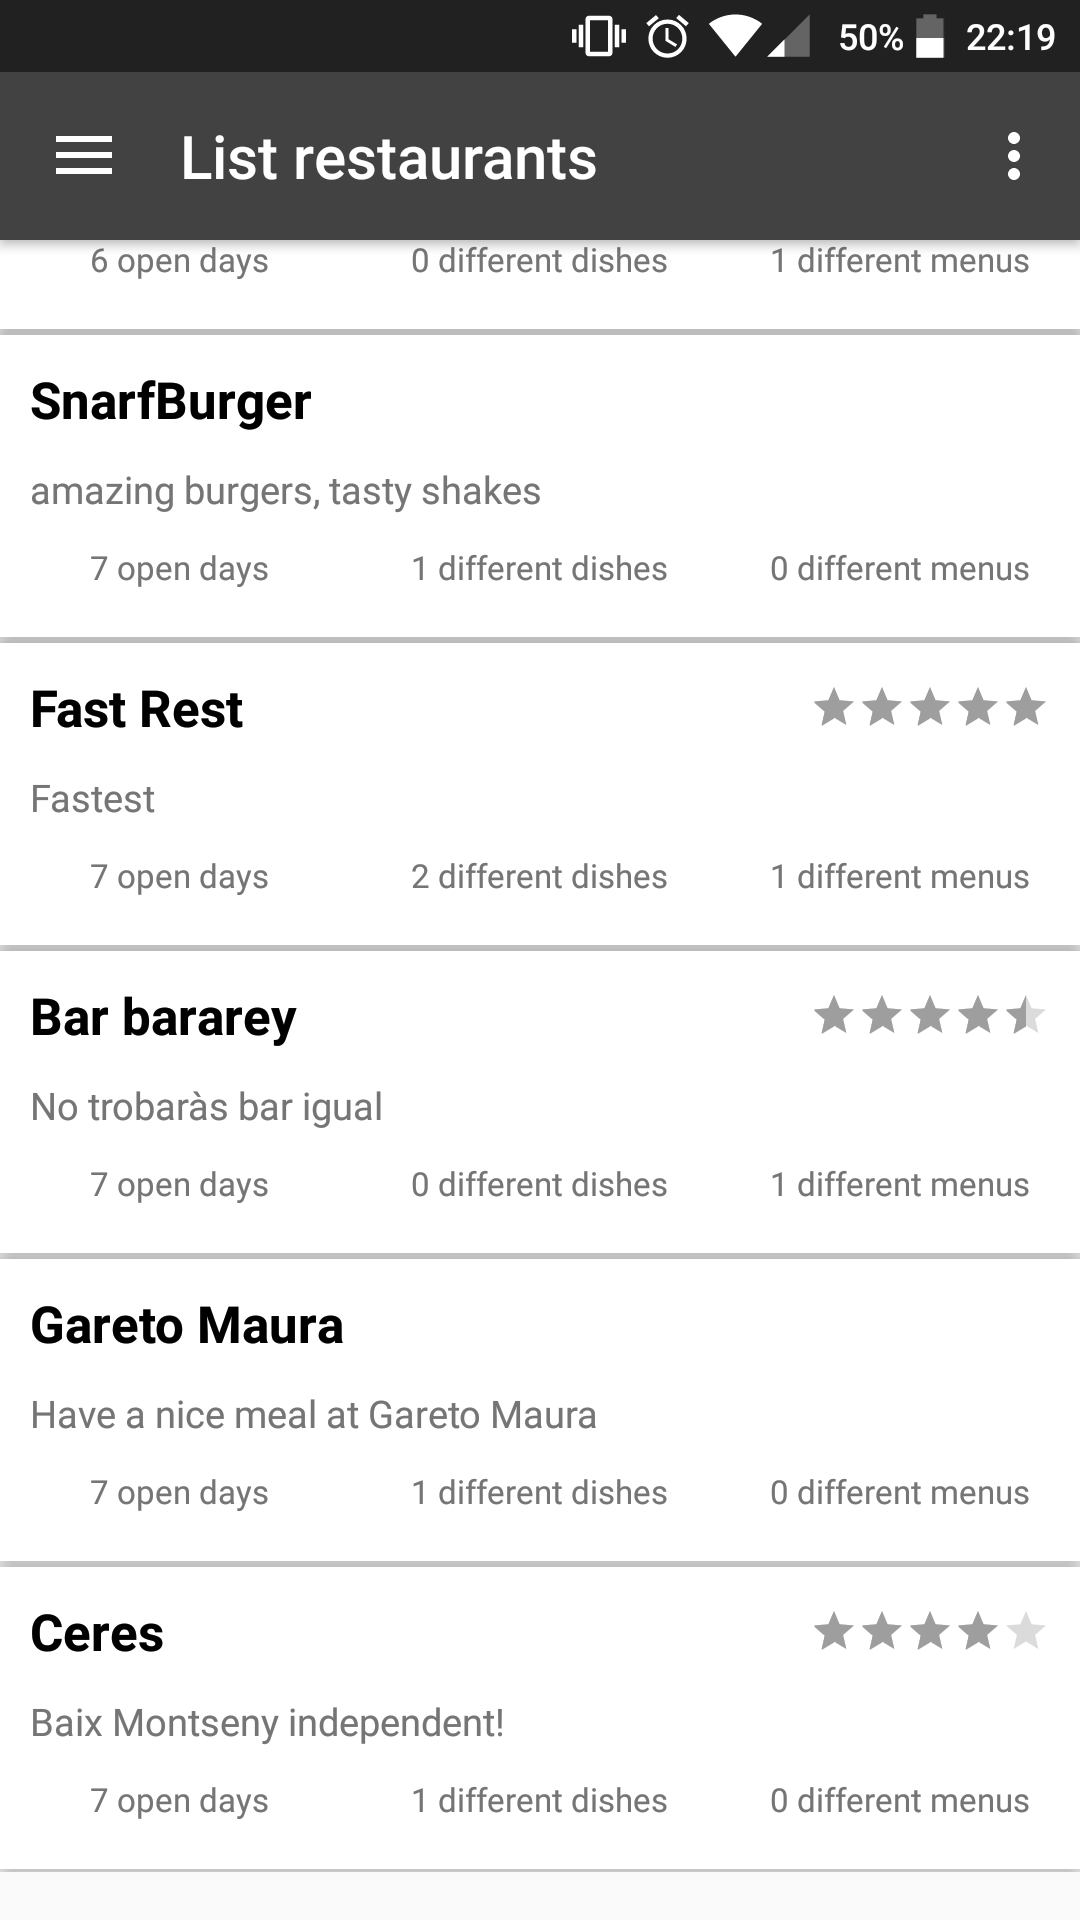
\includegraphics[scale=0.15]{Figures/wisebite_screenshot_1.png}
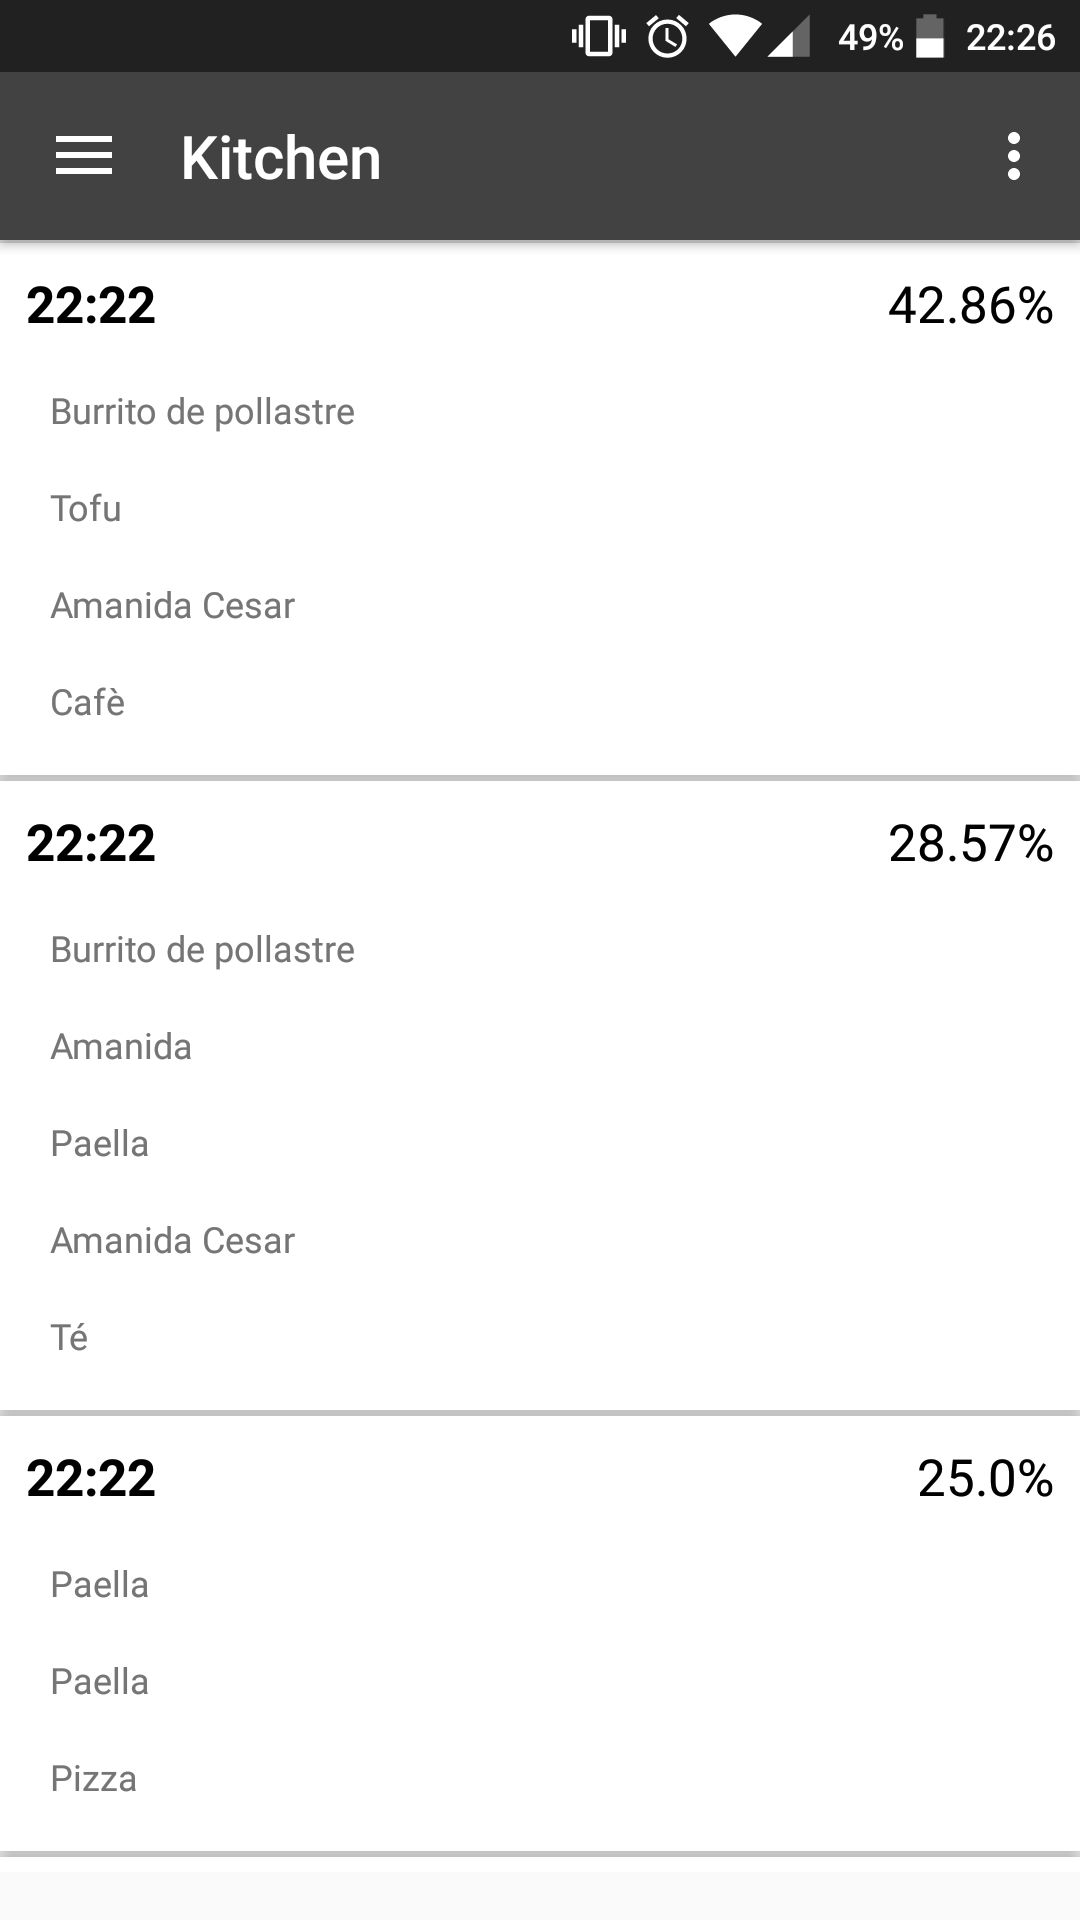
\includegraphics[scale=0.15]{Figures/wisebite_screenshot_2.png}
\caption{Captures de pantalla de Wisebite: llistat de restaurants i mode cuina}
\end{figure}

\begin{figure}[!h]
\centering
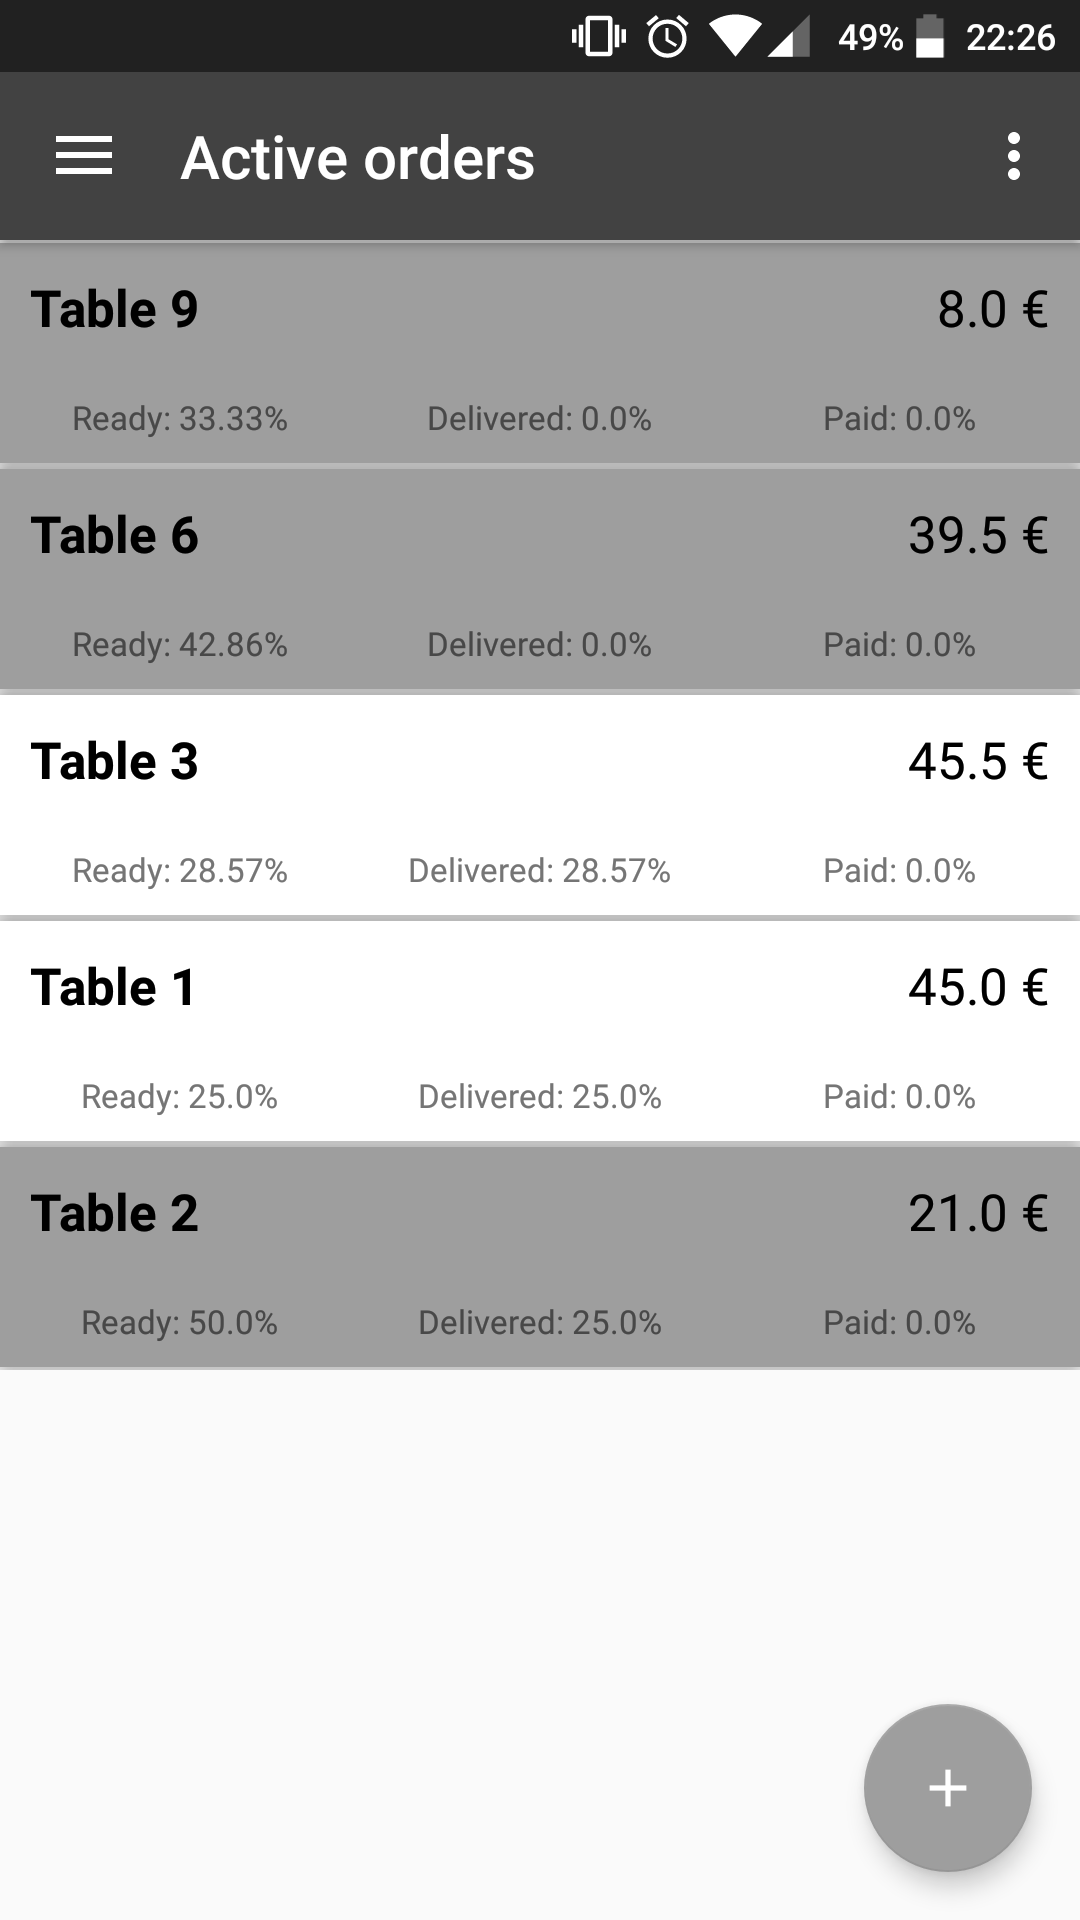
\includegraphics[scale=0.15]{Figures/wisebite_screenshot_3.png}
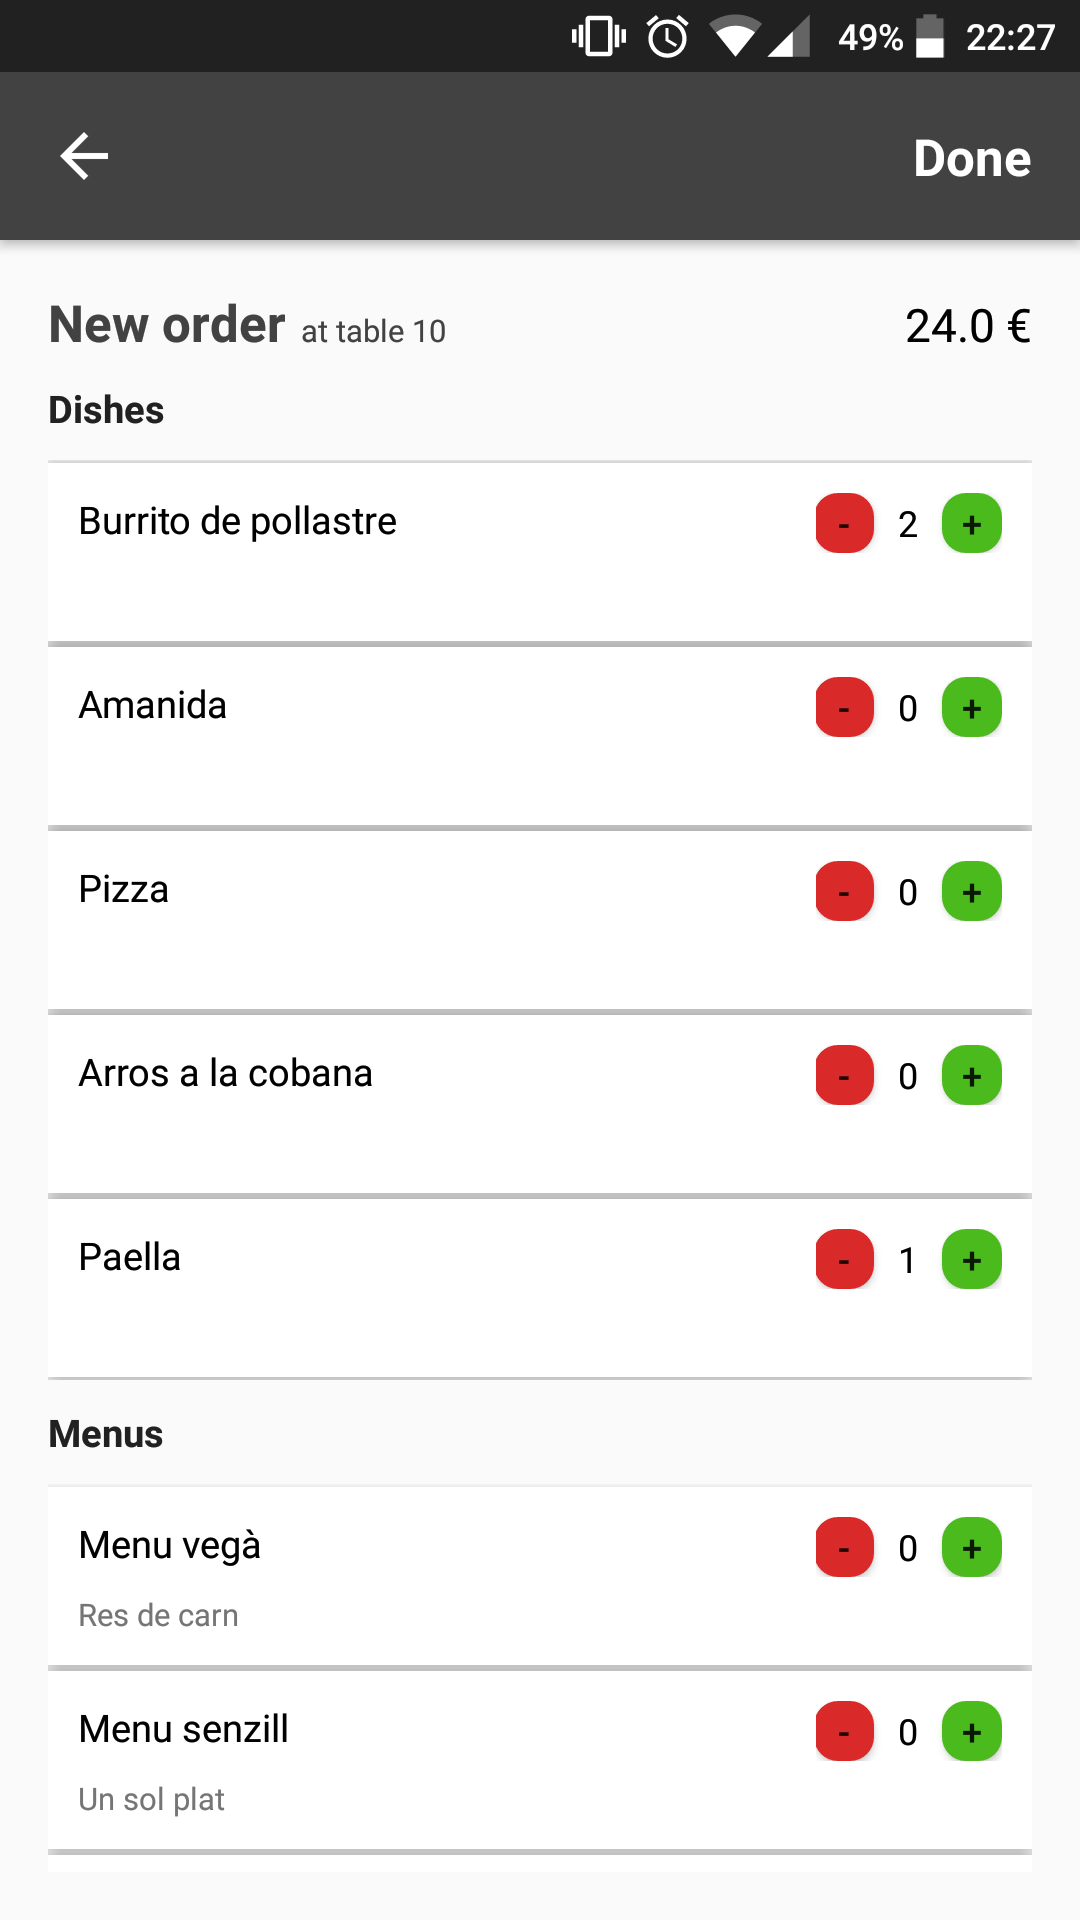
\includegraphics[scale=0.15]{Figures/wisebite_screenshot_4.png}
\caption{Captures de pantalla de Wisebite: llistat de comandes actives i consulta de comanda}
\end{figure}

\begin{figure}[!h]
\centering
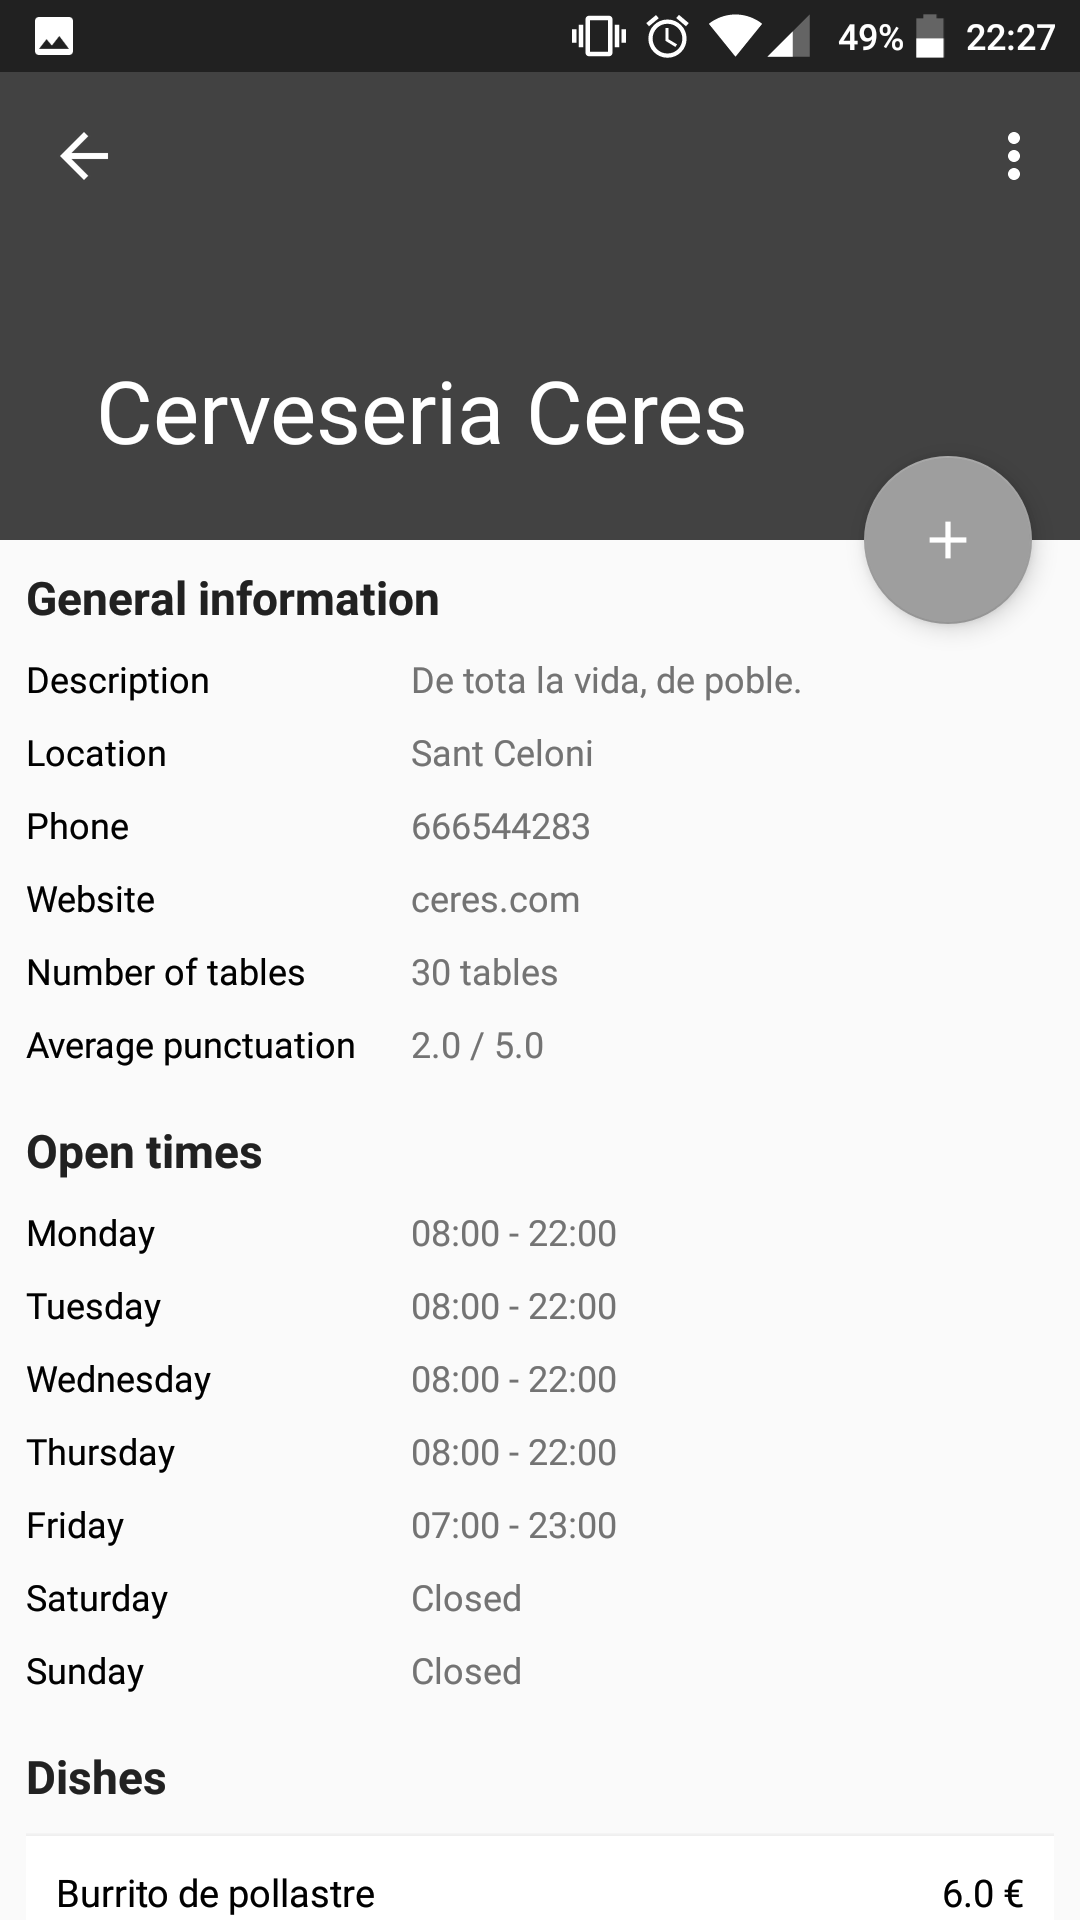
\includegraphics[scale=0.15]{Figures/wisebite_screenshot_5.png}
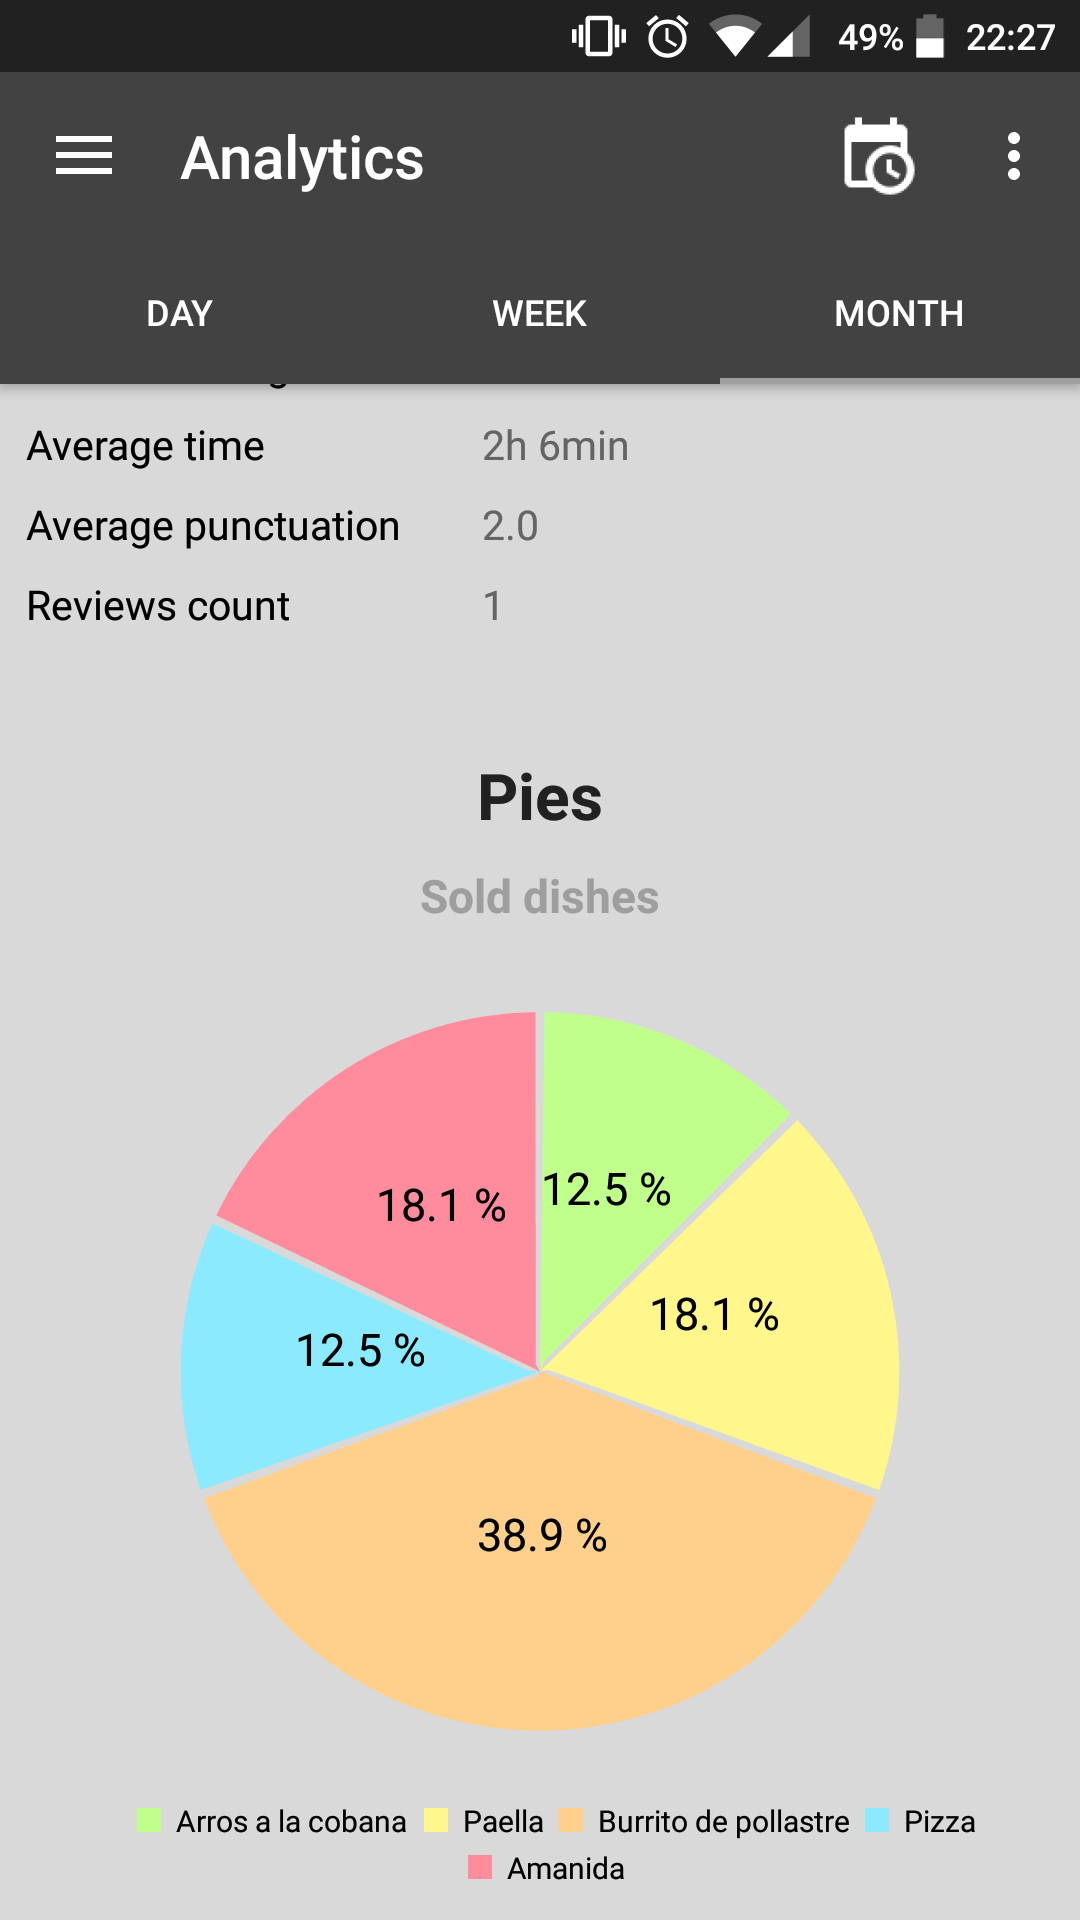
\includegraphics[scale=0.15]{Figures/wisebite_screenshot_6.png}
\caption{Captures de pantalla de Wisebite: consulta de restaurant i estadístiques}
\end{figure}

\begin{figure}[!h]
\centering
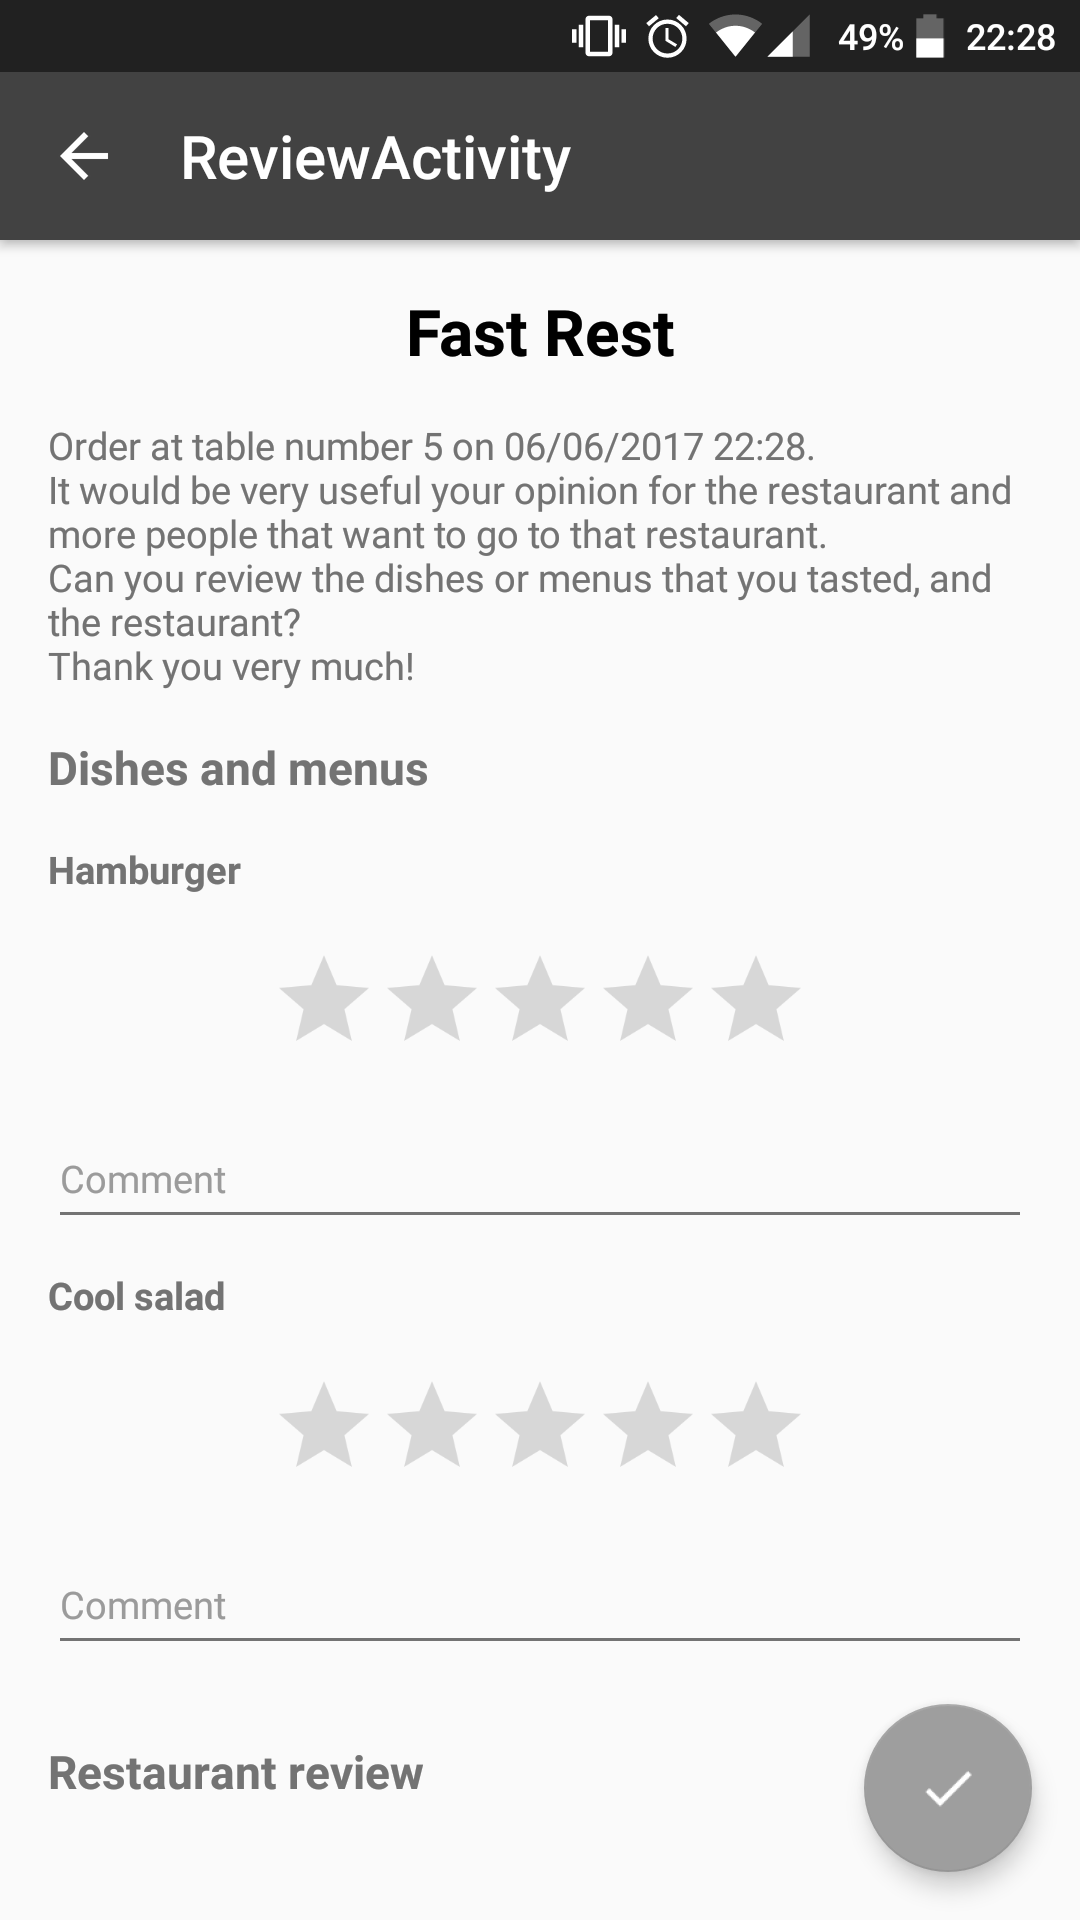
\includegraphics[scale=0.15]{Figures/wisebite_screenshot_7.png}
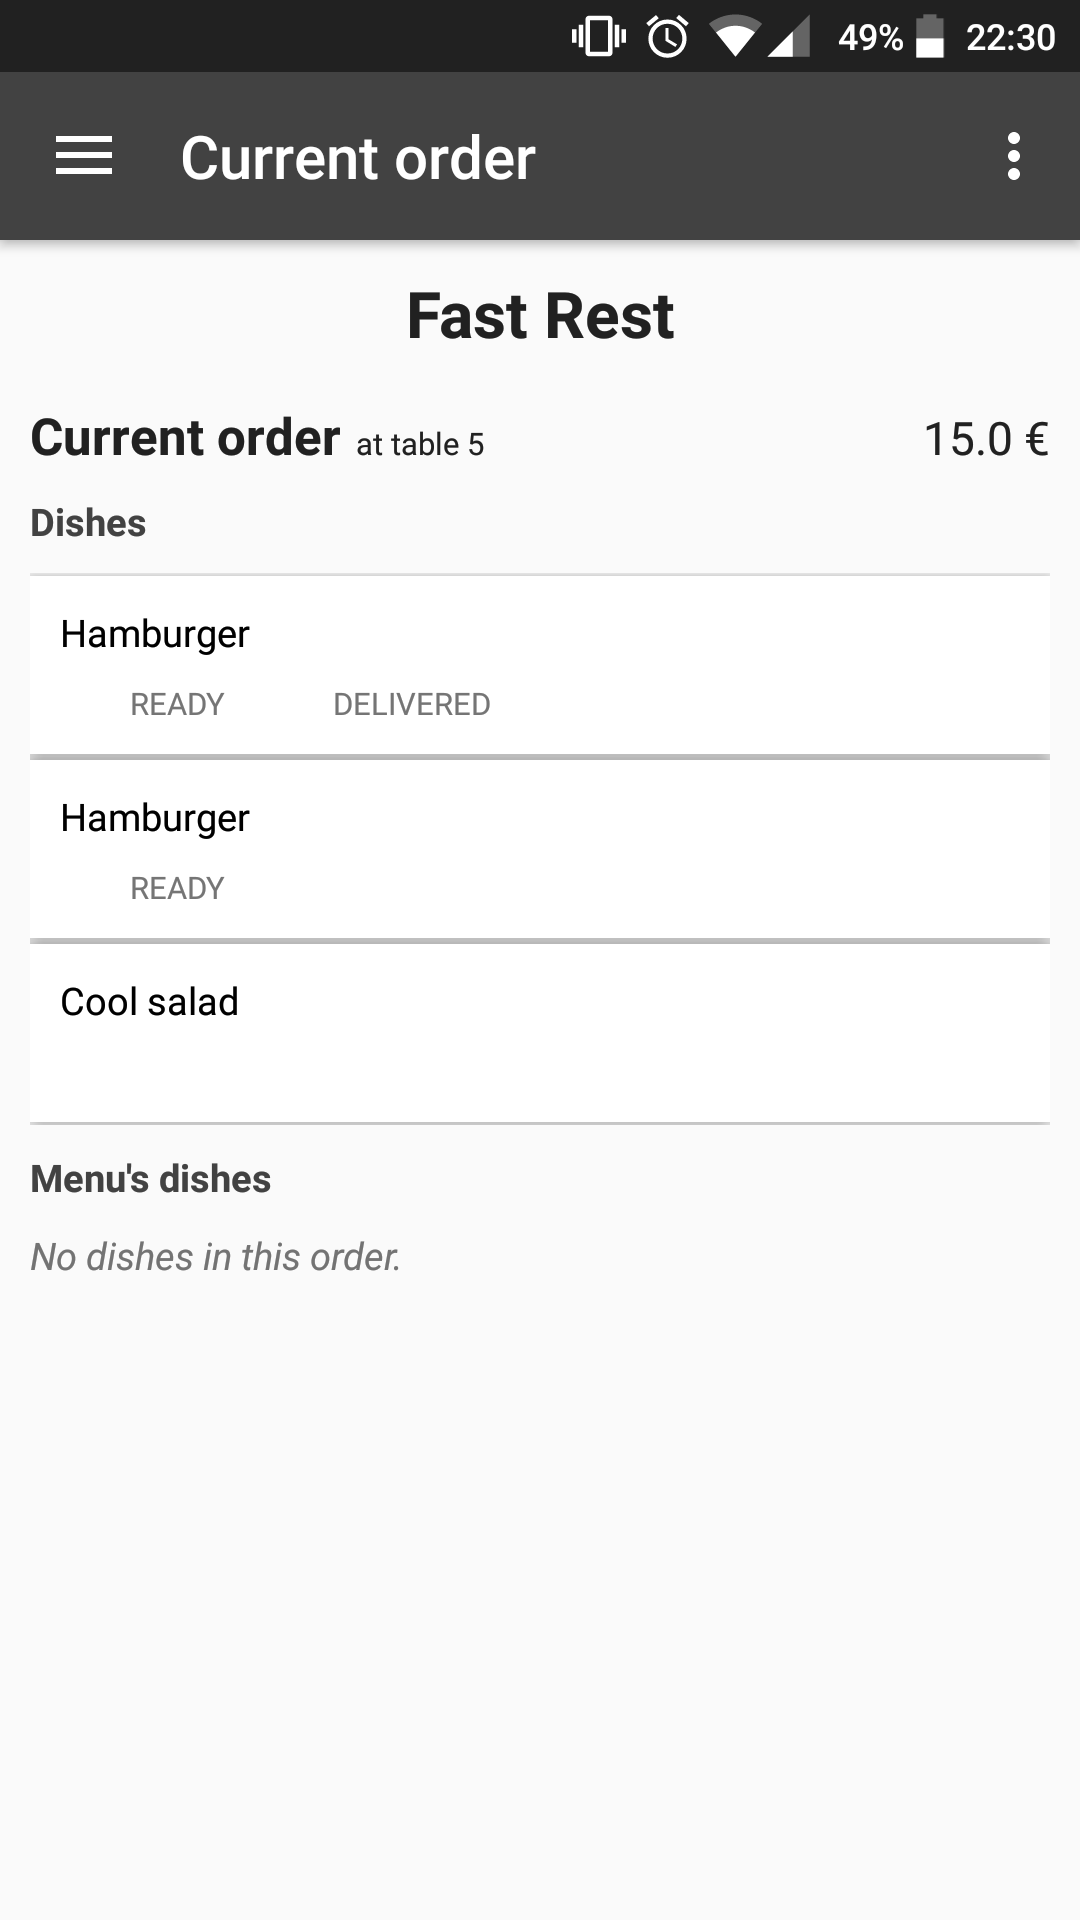
\includegraphics[scale=0.15]{Figures/wisebite_screenshot_8.png}
\caption{Captures de pantalla de Wisebite: valoració i comanda actual}
\end{figure}
% Chapter Template

\chapter{Implementació} % Main chapter title

\label{Chapter7} % Change X to a consecutive number; for referencing this chapter elsewhere, use \ref{ChapterX}

Un cop decidit com serà el sistema, és a dir, quins requisits, objectius i abast tindrà, i quin disseny s'aplicarà en ell, el següent és parla de la implementació per si mateixa. Les decisions preses anteriorment i explicades en capítols anteriors han marcat el que s'explicarà en aquest capítol. En primera instància es realitzarà un repàs per les tecnologies i eines utilitzades durant el desenvolupament de \textit{Wisebite}, i per acabar es seguirà pels detalls de la implementació del projecte.

%----------------------------------------------------------------------------------------
%	SECTION 1
%----------------------------------------------------------------------------------------

\section{Tecnologies i eines utilitzades}

Durant el desenvolupament del projecte s'ha utilitzat tot tipus de tecnologies, és per això que s'ha decidit subdividir-ho en quatre conceptes. Començant pels llenguatges de programació, seguint per les bases de dades, mencionant les eines utilitzades i finalitzant amb les llibreries externes utilitzades.

\subsection{Llenguatge de programació}

\textbf{\large Java}\cite{java}\\
Com es va comentar anteriorment en la decisió de l'arquitectura, es va decidir construir una aplicació Android. Aquest sistema operatiu permet desenvolupar el \textit{backend} de les seves aplicacions natives en Java, C++ i Kotlin. Donat que el desenvolupador tenia més coneixement en desenvolupament d'aplicacions Android en Java, es va decidir utilitzar aquest llenguatge. A més a més, al ser el llenguatge de programació més utilitzat en el món des de ja fa anys, la comunitat d'usuaris és molt gran. En conseqüència, la probabilitat de trobar solucions a possibles problemes que es poden ocasionar és molt més alta que pas amb els altres dos llenguatges.
\\\\
\textbf{\large XML}\cite{xml}\\
El desenvolupament del \textit{frontend} en Android es realitza en llenguatge d'etiquetes, específicament XML. A diferència del \textit{backend}, en aquest cas no es tenia elecció dins del context de desenvolupament d'aplicacions natives.
\\\\
\textbf{\large \LaTeX}\cite{latex}\\
La realització de la memòria del projecte ha estat realitzada amb el llenguatge de software lliure anomenat \LaTeX. És un llenguatge que et permet realitzar documents pdf a través d'unes directives. L'esforç inicial d'aprendre aquest llenguatge es va contemplar en la planificació temporal del projecte, i tot i conèixer que seria d'un període més o menys considerable, es va contemplar l'esforç com útil en el projecte per la professionalitat i la robustesa que reflexa el document.
\\\\
\begin{figure}[H]
\centering

\includegraphics[scale=0.20]{Figures/java.png}

\includegraphics[scale=0.15]{Figures/xml.png}
\hspace{0.8cm}

\includegraphics[scale=0.20]{Figures/latex.png}
\caption{Llenguatges de programació}
\end{figure}

\subsection{Bases de dades}

TODO: Redactar

\subsection{Eines}

TODO: Redactar

\subsection{Llibreries externes}

TODO: Redactar

%----------------------------------------------------------------------------------------
%	SECTION 2
%----------------------------------------------------------------------------------------

\section{Detalls de la implementació}

TODO: Redactar

\subsection{Implementació de l'aplicació}

TODO: Redactar

\subsection{Implementació de la memòria}

TODO: Redactar

% Chapter Template

\chapter{Avaluació del sistema} % Main chapter title

\label{Chapter8} % Change X to a consecutive number; for referencing this chapter elsewhere, use \ref{ChapterX}

%----------------------------------------------------------------------------------------
%	SECTION 1
%----------------------------------------------------------------------------------------

\section{Proves durant el desenvolupament}

Lorem ipsum dolor sit amet, consectetur adipiscing elit. Aliquam ultricies lacinia euismod. Nam tempus risus in dolor rhoncus in interdum enim tincidunt. Donec vel nunc neque. In condimentum ullamcorper quam non consequat. Fusce sagittis tempor feugiat. Fusce magna erat, molestie eu convallis ut, tempus sed arcu. Quisque molestie, ante a tincidunt ullamcorper, sapien enim dignissim lacus, in semper nibh erat lobortis purus. Integer dapibus ligula ac risus convallis pellentesque.

%----------------------------------------------------------------------------------------
%	SECTION 2
%----------------------------------------------------------------------------------------

\section{Proves finals}

Sed ullamcorper quam eu nisl interdum at interdum enim egestas. Aliquam placerat justo sed lectus lobortis ut porta nisl porttitor. Vestibulum mi dolor, lacinia molestie gravida at, tempus vitae ligula. Donec eget quam sapien, in viverra eros. Donec pellentesque justo a massa fringilla non vestibulum metus vestibulum. Vestibulum in orci quis felis tempor lacinia. Vivamus ornare ultrices facilisis. Ut hendrerit volutpat vulputate. Morbi condimentum venenatis augue, id porta ipsum vulputate in. Curabitur luctus tempus justo. Vestibulum risus lectus, adipiscing nec condimentum quis, condimentum nec nisl. Aliquam dictum sagittis velit sed iaculis. Morbi tristique augue sit amet nulla pulvinar id facilisis ligula mollis. Nam elit libero, tincidunt ut aliquam at, molestie in quam. Aenean rhoncus vehicula hendrerit.
% Chapter Template

\chapter{Planificació temporal} % Main chapter title

\label{Chapter9} % Change X to a consecutive number; for referencing this chapter elsewhere, use \ref{ChapterX}

Abans d'iniciar qualsevol projecte, com pot ser aquest treball final de grau, s'ha de dur a terme una anàlisi acurada de la feina a realitzar i quins són els recursos i temps dels quals es disposa per dur-ho a terme. Si es porta a la pràctica una bona anàlisi, sortirà com a resultat una bona planificació inicial que s'adaptarà a la realitat durant tot el transcurs del projecte. Tot i així sempre poden sorgir imprevistos que poden variar la planificació inicial i posar en risc el producte final que es pretén construir. En aquest capítol es presentarà la planificació inicial que es va realitzar, els possibles pla d'acció en cas d'alteracions i el que realment ha passat, és a dir, com ha anat la planificació i si hi ha hagut desviacions.

%----------------------------------------------------------------------------------------
% SECTION 1
%----------------------------------------------------------------------------------------

\section{Calendari}

La durada del treball final de grau és de quatre mesos i mig, és a dir, unes 18 setmanes. Comença el 13 de febrer amb l'inici del quadrimestre i acaba entre els dies 26 i 30 de juny amb la defensa oral del projecte. Tot i així, es podrà donar el projecte per finalitzat una setmana abans amb l'entrega de la memòria final perquè el director i ponents del projecte tinguin temps per analitzar-ho amb deteniment.
\\\\
Cal dir per això que poden sorgir inconvenients durant el transcurs del projecte que alterin la planificació inicial planejada, o per altra banda, haver planificat a la baixa i finalitzar-lo abans de l'esperat. Tot i així, es realitzaran controls periòdics per controlar acordament que la planificació no se surti de la ruta esperada i, en cas que ho faci, corregir el rumb per adaptar-se.
\\\\
Cal mencionar en la planificació, que es té en compte el fet que l'estudiant està cursant altres assignatures i que en períodes esporàdics del quadrimestre hagi de dedicar més temps a tasques d'aquestes, i que en conseqüència deixi en \textit{Stand by} les tasques relacionades amb el treball final de grau.

%----------------------------------------------------------------------------------------
% SECTION 2
%----------------------------------------------------------------------------------------

\section{Recursos}

Durant l'execució d'un projecte, sempre hi ha un ús d'un conjunt de recursos. Per a la descripció d'aquests recursos necessaris per a la realització d'aquest projecte, cal especificar que existeixen tres grups de recursos: personals, materials i de software.

\clearpage
\subsection{Recursos personals}

Durant el període comentat anteriorment, l'estudiant i autor del projecte li dedicarà unes 30 hores setmanals al desenvolupament i realització del treball final de grau. A més a més, se li afegeix l'ajut en correccions, assessorament i seguiment del director d'aquest.

\subsection{Recursos materials}

Serà necessària la presència d'un lloc de treball físic per dur a terme el projecte. Aquest lloc de treball pot ser únic o variat segons la disponibilitat de l'estudiant en aquell moment. A més a més, això comportarà costos extres com per exemple electricitat.
\\\\
Per a la implementació i redacció de la documentació serà necessària la disponibilitat completa d'un ordinador, tant sigui portàtil com de sobretaula. Aquest ordinador haurà de tenir instal·lat tot el programari necessari per construir el projecte. Serà necessari incloure un cost extra per instal·lar dit programari.
\\\\
A més a més, com a últim recurs material, també tenir en compte els servidors en els quals s'emmagatzemarà les dades que utilitzarà la plataforma per funcionar, concretament \textit{Firebase} com s'ha comentat anteriorment.

\subsection{Recursos de software}

Durant tota l'execució del treball final de grau s'utilitzarà un gran nombre de programes software, que seran necessaris per a la realització d'aquest. Un grapat d'aquest programari software ha estat comentat amb més detall en apartats anteriors.
\\\\
En primer terme, s'utilitzarà alguna de les aplicacions disponibles a \textit{Google Apps}\cite{gsuite} com \textit{Drive}, \textit{Docs}, \textit{Sheets} o \textit{Slides}. Totes elles ajudaran a poder redactar la documentació del projecte i emmagatzemar tot ella en un mateix lloc multiplataforma.
\\\\
Per altra banda, en ser una aplicació Android, s'utilitzarà l'entorn de desenvolupament Android Studio\cite{androidstudio}, recomanat pel mateix Google. Amb l'ajut de la seva interfície gràfica, plugins i el IDE en si mateix, facilitarà molt la construcció de la plataforma \textit{Wisebite}.
\\\\
Encara que el treball final de grau no sigui un treball en equip, sinó individual, això no menysprea l'ús d'un control de versions. En aquest projecte s'utilitzarà Git com a eina, i estarà emmagatzemada als servidors de \textit{GitHub}\cite{github}. Amb aquesta eina serà més fàcil poder gestionar l'evolució de l'aplicació i poder recuperar versions antigues.
\\\\
Per últim, en aplicar una metodologia àgil s'utilitzarà \textit{Trello}\cite{trello} per a la gestió i control del projecte. Amb la capacitat de crear targetes dins d'un llistat i associar-li un pes, facilita en gran mesura la implantació de Scrum en aquest projecte.

%----------------------------------------------------------------------------------------
% SECTION 3
%----------------------------------------------------------------------------------------

\section{Descripció de les tasques}

Una part imprescindible per a la planificació temporal del projecte és realitzar una anàlisi molt detallada de les tasques a realitzar durant les tres fases del treball final de grau. Marcant èmfasi en el fet que aquest projecte estarà sota els ideals de la metodologia àgil, per tant, funcionarà via històries d'usuari i iteracions o sprints del projecte. Tota aquesta informació serà explicada a continuació.

\subsection{Fase inicial}

La primera part del projecte es basa en l'especificació general del que es vol construir. En aquesta fase inicial es detallarà el context, estudi de l'art i l'abast per una banda, la planificació temporal i la descripció de les tasques per altra i per últim un informe sobre la gestió econòmica i sostenibilitat del projecte.
\\\\
A més a més d'això, seguint la metodologia Scrum, es crearà el \textit{backlog} inicial del projecte. Un backlog ve a ser un llistat d'històries d'usuari que componen la plataforma, on cada història d'usuari és una característica o funcionalitat de l'aplicació totalment independent a la resta. A cada una d'aquestes històries d'usuari se li haurà d'atribuir un pes valorant el cost que tindrà la seva implementació. Un cop definits aquests pesos serà molt més fàcil poder prioritzar les tasques a realitzar. Una història d'usuari es donarà per finalitzada quan compleixi cada un dels criteris d'acceptació que haurà de tenir dins la targeta de cada història d'usuari.
\\\\
Un cop definit tot això passarem a la següent fase del projecte. Cal tenir cura en realitzar una bona fase inicial, ja que pot condicionar de manera notable el procés del projecte.

\subsection{Iteracions del projecte}

Seguint la metodologia Scrum, s'haurà d'aplicar el desenvolupament incremental i vertical, és a dir, anar implementant les funcionalitats o característiques de la plataforma ordenant-les per prioritat. Per a portar-ho a la pràctica es durà a terme un seguit de cinc sprints o iteracions. A final de cada sprint, tindrem una versió de la plataforma que funcioni i es pugui entregar a un hipotètic client.
\\\\
Un sprint es compon d'un seguit d'històries d'usuari ponderades. L'objectiu és aconseguir que totes elles compleixin els criteris d'acceptació al final del període de l'sprint.
\\\\
El primer sprint comença el 13 de març i tindrà una durada de dues setmanes, com cada un dels quatre sprints restants. Seguint a aquest ritme, està previst finalitzar la cinquena i última iteració per al 22 de maig. Inicialment es planificaran les iteracions perquè totes elles ponderin aproximadament el mateix. Tot i així, segons la velocitat que es vegi en el desenvolupament d'aquestes històries, es replantejarà o no en la retrospectiva que sempre es farà a final d'sprint.
\\\\
Tot i que el 22 de maig encara quedarà un mes per a la lectura del treball final de grau, l'objectiu és finalitzar la implementació per aquelles dates. Així es tindrà suficient temps per dedicar-li a la fase final de projecte.

\subsection{Fase final}

Un cop s'hagi finalitzat les cinc iteracions del projecte es passarà a la fase final d'aquest. En aquesta etapa es redactarà la memòria i la documentació necessària per al projecte. Es disposarà pràcticament d'un mes per a meditar i construir una bona documentació, i preparar la lectura que es tindrà a finals del mes de juny.

%----------------------------------------------------------------------------------------
% SECTION 4
%----------------------------------------------------------------------------------------

\section{Diagrama de Gantt}

Un cop analitzat el calendari del qual disposem, els recursos que seran utilitzats i la descripció detallada de les tasques a realitzar, és important adjuntar el diagrama de Gantt\cite{gantt}. Així es podrà disposar d'una visió completa de quina és la planificació inicial del projecte. Aquest diagrama està adjunt a l'apèndix \ref{Gantt}.

%----------------------------------------------------------------------------------------
% SECTION 5
%----------------------------------------------------------------------------------------

\section{Valoració d'alternatives i pla d'acció}

Durant el desenvolupament del projecte poden sorgir imprevistos que impediran la construcció d'aquest. Pot haver-hi dos tipus de desviacions: mala planificació de temps o imprevistos inesperats o personals.
\\\\
En primer cas, la mala planificació de temps, pot esdevenir de dues maneres. Per una banda, que hagi estat a l'alça. En aquest cas no hi hauria massa problemàtica, ja que si s'acabessin les històries d'una iteració abans de la data límit, s'afegirà la següent història d'usuari del backlog amb esperances de poder finalitzar dins l'sprint. En canvi, per altra banda, pot sorgir que s'hagi estimat a la baixa. En aquest cas, s'intentarà aplicar unes hores extres en el desenvolupament de les històries pendents o, en cas que sigui impossible, deixar-les per fer i replantejar els següents sprints en la retrospectiva.
\\\\
En segon lloc, ens podem trobar amb algun imprevist inesperat o bé personal. En casos com aquest, s'analitzarà el cas en especial, ja que pot sorgir qualsevol tipus de problema. Un cop analitzat, se li intentarà donar una solució amb l'objectiu de poder finalitzar de forma correcta la iteració en la qual estiguem situats. En cas que sigui impossible, es tractarà el tema en concret amb el director del projecte.

%----------------------------------------------------------------------------------------
% SECTION 6
%----------------------------------------------------------------------------------------

\section{Planificació definitiva}

En la primera fase del projecte es va realitzar una planificació inicial a on s'especificava quines tasques es realitzarien durant el Treball Final de Grau, com s'organitzarien i, sobretot, quant temps es dedicaria en cada una d'elles. Després d'haver transcorregut i haver finalitzat el projecte, hi ha hagut punts que es van estimar correctament i s'han pogut dur a terme sense cap tipus de problemàtica però d'altres que s'han vist forçats a modificar. Un cop analitzats es veurà si finalment, fent balanç, ha modificat l'objectiu final de projecte.

\subsection{Acord amb la planificació inicial}

En el seu moment es va definir una metodologia de treball inspirada en la metodologia àgil Scrum, amb un seguit de cinc sprints o iteracions a on es desenvoluparia la implementació del projecte. L'objectiu era definir un \textit{backlog} inicial amb totes les \textit{històries d'usuari} que contindria el projecte i, en cada un dels \textit{sprint plannings}, atribuir un conjunt d'aquestes a aquell sprint.
\\\\
Després d'aquests d'implementar el projecte es pot dir que s'ha seguit aquest patró o metodologia de treball. A més a més, comentar que la durada de les dues setmanes per iteració que es va atribuir a la planificació inicial s'ha respectat amb una variació màxima de 2 o 3 dies.
\\\\
Tot i així, es va decidir repartir les històries d'usuari segons la disponibilitat de la qual disposava l'alumne per implementar-les durant el període de l'sprint. Malgrat aquesta decisió, el conjunt de les cinc iteracions ha complert amb la planificació inicial.

\subsection{Modificacions}

El canvi més important que s'ha realitzat acord amb la planificació inicial del projecte, però que no modifica el fet d'arribar a l'objectiu final en el temps acordat, és l'alteració en l'ordre de les tasques. En el seu moment es va estipular la idea de realitzar durant dos mesos tota la implementació del projecte i, en l'últim més, redactar la memòria documentant tota la implementació realitzada durant la fase intermèdia.
\\\\
El canvi ha estat degut per un seguit de factors. Tant el director del projecte com l'alumne que el porta a càrrec es van adonar que realitzar l'ordre de tasques estipulat inicialment portaria a la problemàtica de no tenir una bona documentació final a entregar. En primer lloc pel poc temps que es disposava en comparació del que es necessita per realitzar una bona memòria, i per altra banda el fet de documentar tot al final podria donar lloc a no realitzar una documentació de la implantació del tot acurada donat el temps entre finalitzar el codi i explicar-lo. A més a més, el fet d'anar intercalant implementació amb documentació faria més amè el transcurs del projecte.
\\\\
Per altra banda, hi ha hagut modificacions en la implementació de les \textit{històries d'usuari}. Inicialment, en realitzar i definir \textit{backlog} inicial, es van crear un seguit de \textit{features} sense contemplar del tot el temps que es disposava per implementar-les. Llavors, durant la realització de la iteració, l'alumne es va adonar que aquestes històries d'usuari aportaven un esforç extra en l'sprint que no es veia reflectit en el resultat final. És a dir, l'esforç que es necessitava per implementar aquestes històries d'usuari no era equivalent al valor que aportava a l'usuari final del producte. En conseqüència, per tal de solucionar aquesta problemàtica, es va decidir presidir d'aquestes \textit{features} donat el temps acotat del projecte.

\subsection{Conclusions}

Finalment, es pot considerar que tot i les modificacions en comparació de la planificació inicial, no hi ha hagut cap problemàtica en arribar de forma correcta al \textit{deadline} del projecte. Ja amb el projecte finalitzat, s'ha implementat les tres fases del treball, corresponents als tres punts que definien l'abast del projecte: gestió interna de l'establiment, anàlisi del restaurant i interacció del client.
\\\\
Paral·lelament s'ha documentat la memòria dins el temps establert i ha donat temps a una revisió detallada d'aquesta.
\\\\
Per fer-se una idea de com ha anat l'evolució tant del codi de l'aplicació com el de la memòria, s'adjunta a continuació dues gràfiques proporcionades per \textit{GitHub} que mostren el temps de dedicació a cada una de les dues tasques: codi i memòria.

\begin{figure}[H]
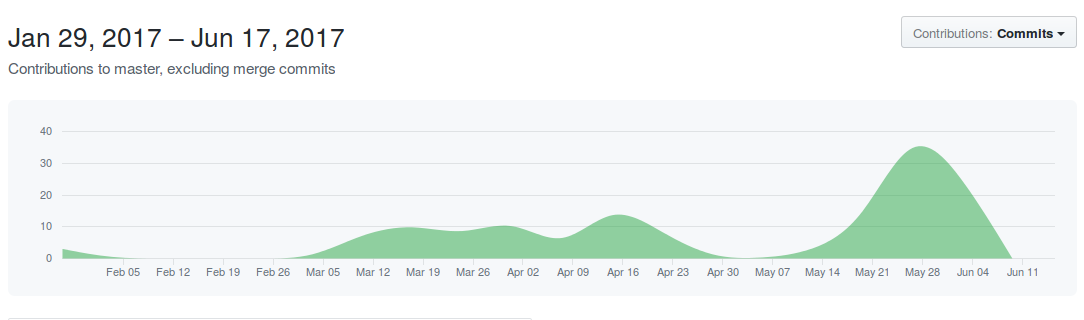
\includegraphics[scale=0.375]{Figures/commits_android.png}
\caption{Contribucions en el codi de l'aplicació}
\end{figure}
\begin{figure}[H]
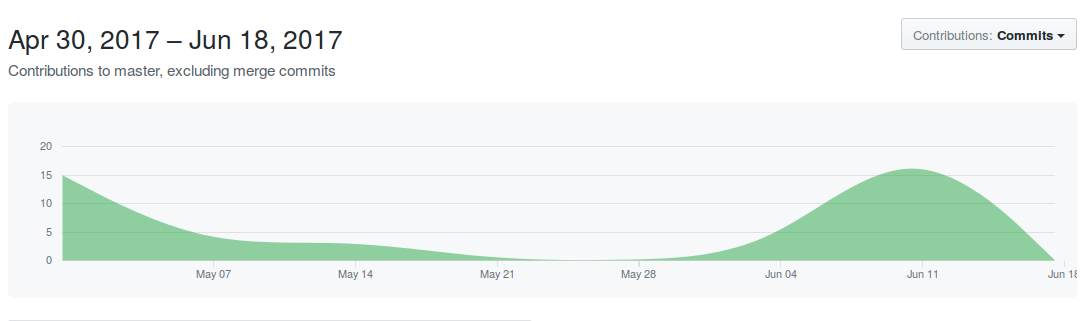
\includegraphics[scale=0.375]{Figures/commits_reports.png}
\caption{Contribucions en la memòria}
\end{figure}
% Chapter Template

\chapter{Gestió econòmica} % Main chapter title

\label{Chapter10} % Change X to a consecutive number; for referencing this chapter elsewhere, use \ref{ChapterX}

En aquest apartat es tractarà el cost econòmic que causarà la construcció d'aquest projecte. El treball final de grau és un projecte no remunerat, és a dir, que l'estudiant no rebrà cap recompensa econòmica per a la realització d'aquest. Tot i així, suposarem l'existència d'un equip de treball compost per un cap de projecte, un grup d'analistes i dissenyadors i un conjunt de programadors i provadors. Per així simular quin cost tindria un projecte d'aquest tipus en cas de ser part d'una \textit{startup}.

%----------------------------------------------------------------------------------------
% SECTION 1
%----------------------------------------------------------------------------------------

\section{Identificació i estimació de costos}

Per a la construcció del pressupost\cite{presupuesto} d'aquest projecte es necessita tenir en compte els costos directes, que representen als recursos humans, els costos indirectes, que es reflecteixen als recursos materials, i a les contingències i imprevistos. Tots ells, després de la seva anàlisi, esdevindran al pressupost final d'aquest projecte.

\subsection{Costos directes}

Els costos directes són el conjunt de despeses que corresponen al grup de recursos humans que necessita el projecte. Tot i que aquest projecte, com s'ha comentat abans, no té cap tipus de remuneració, es fa només amb afany acadèmic i és només individual, suposarem l'existència d'un equip de treball qualificat econòmicament. Per apropar-nos més al mercat s'ha assignat un responsable d'equip a cada una de les tasques reflectides al diagrama de \textit{Gantt}. S'ha estimat que el cap de projecte tindrà un salari al voltant dels 45\euro/hora, el grup d'analistes i dissenyadors 35\euro/hora i l'equip de programadors i provadors de 20\euro/hora.
\\\\
Aleshores, com a resultant d'aquesta anàlisi sorgeix la taula següent amb la quantitat d'hores, cost unitari i total de cada una de les activitats del projecte.
\\
\begin{table}[H]
\centering
\begin{tabular}{ | l | r | r | r |}
\hline
\textbf{ACTIVITAT}&\textbf{HORES}&\textbf{COST UNITARI}&\textbf{COST TOTAL} \\ \hline
Recerca i plantejament de la idea & 15h & 45\euro/hora & 675\euro \\ \hline
Fase inicial & 75h & 45\euro/hora & 3.375\euro \\ \hline
Sprint 1: disseny & 10h & 35\euro/hora & 350\euro \\ \hline
Sprint 1: implementació & 30h & 20\euro/hora & 600\euro \\ \hline
Sprint 2: disseny & 10h & 35\euro/hora & 350\euro \\ \hline
Sprint 2: implementació & 30h & 20\euro/hora & 600\euro \\ \hline
Sprint 3: disseny & 10h & 35\euro/hora & 350\euro \\ \hline
Sprint 3: implementació & 30h & 20\euro/hora & 600\euro \\ \hline
Sprint 4: disseny & 10h & 35\euro/hora & 350\euro \\ \hline
Sprint 4: implementació & 30h & 20\euro/hora & 600\euro \\ \hline
Sprint 5: disseny & 10h & 35\euro/hora & 350\euro \\ \hline
Sprint 5: implementació & 30h & 20\euro/hora & 600\euro \\ \hline
Fase final & 50h & 45\euro/hora & 2.250\euro \\ \hline
\textbf{TOTAL} & 340h & --- & 11.050\euro \\
\hline
\end{tabular}
\caption{Costos directes}
\end{table}
\noindent Les hores calculades per activitat s'han calculat amb el supòsit que ha d'haver-hi un treball, en mitjana, de 30 hores setmanals dedicades al projecte. Finalment, hi haurà una dedicació humana de 340 hores, amb un cost de 11.050\euro\space considerant els supòsits anteriors.

\subsection{Costos indirectes}

Durant tot el projecte apareixeran situacions quotidianes que repercutiran en el pressupost final amb connotativa indirecte com els que s'exposen a continuació.
\\\\
En primer terme, s'ha de valorar la connexió a Internet com a cost indirecte. El seu cost mensual és de 33\euro, no obstant s'ha de tenir en compte que no s'utilitzarà el 100\% del seu ús en tasques relacionades amb el treball final de grau. Per això se li atribueix un 30\% de dedicació.
\\\\
En segon lloc, s'ha de valorar el hardware utilitzat. En aquest projecte només s'utilitzarà un portàtil per al desenvolupament i construcció del projecte i, addicionalment, un telèfon mòbil amb sistema operatiu Android per a realitzar les proves pertinents segons vagi evolucionant el producte. El cost del portàtil se situa als 500\euro\space juntament amb els 310\euro\space del telèfon mòbil. No obstant això, es considera una vida útil de 4 anys per al portàtil i de 2 anys i mig per al mòbil. Per tant, se li atribueix un 10\% i un 17\% de dedicació a cada un dels dispositius tecnològics respectivament.
\\\\
Per últim no oblidar-nos de les impressions en paper que es realitzaran durant el projecte. Tant durant el desenvolupament d'aquest com en la memòria final s'imprimirà documentació. S'ha valorat que s'utilitzaran 500 impressions durant tot el projecte a 0.05\euro\space la unitat.
\\
\begin{table}[H]
\centering
\begin{tabular}{ | l | r | r | r |}
\hline
\textbf{ACTIVITAT}&\textbf{COST}&\textbf{DEDICACIÓ}&\textbf{COST TOTAL} \\ \hline
Internet & 33\euro & 30\% & 10\euro \\ \hline
Hardware: Portàtil & 500\euro & 10\% & 50\euro \\ \hline
Hardware: Telèfon mòbil & 310\euro & 17\% & 53\euro \\ \hline
Impressions & 25\euro & 100\% & 25\euro \\ \hline
\textbf{TOTAL} & --- & --- & 138\euro \\
\hline
\end{tabular}
\caption{Costos indirectes}
\end{table}

\subsection{Contingències}

En tot pressupost sempre s'ha de reservar un 15\% de contingències, que s'aplicaran tant en els costos directes com indirectes.
\\
\begin{table}[H]
\centering
\begin{tabular}{ | l | r | r | r |}
\hline
\textbf{ACTIVITAT}&\textbf{COST}&\textbf{PERCENTATGE}&\textbf{COST TOTAL} \\ \hline
Costos directes & 11.050\euro & 15\% & 12.708\euro \\ \hline
Costos indirectes & 138\euro & 15\% & 159\euro \\ \hline
\textbf{TOTAL} & --- & --- & 12.867\euro \\
\hline
\end{tabular}
\caption{Contingències}
\end{table}

\subsection{Imprevistos}

Durant el transcurs del desenvolupament del projecte és possible que apareguin imprevistos que afectin el pressupost.
\\\\
El primer es considera la mala planificació en temps del projecte. Pot donar-se el cas en què algunes setmanes s'hagi d'invertir més temps en la programació i desenvolupament de la plataforma per complir els terminis establerts en la planificació inicial. S'ha valorat afegir unes 30 hores extres durant tot el projecte, les quals seran atribuïdes al paper de programador o provador, recordant el seu salari de 20\euro/hora. Per tant, es valora aquest cost addicional amb 600\euro.
\\\\
L'altre possible imprevist que es pot trobar el projecte és alguna incidència amb el hardware utilitzat, és a dir, l'ordinador portàtil o el telèfon mòbil. S'ha valorat en 150\euro\space la possible reparació davant d'un presumpte problema que impedeixi el desenvolupament d'aquest projecte.
\\
\begin{table}[H]
\centering
\begin{tabular}{ | l | r |}
\hline
\textbf{ACTIVITAT} &\textbf{COST} \\ \hline
Hores extra & 600\euro \\ \hline
Incidència amb el hardware & 150\euro \\ \hline
\textbf{TOTAL} & 750\euro \\
\hline
\end{tabular}
\caption{Imprevistos}
\end{table}

\subsection{Pressupost final}

Per a la realització del pressupost final no s'ha tingut en compte cap tipus de variació en els costos, com podria ser l'augment de salaris, donat que el projecte és de curta durada. Per altra banda no s'ha tingut en compte cap tipus d'amortització o marge de benefici donat que és un projecte de caràcter acadèmic sense ànim de lucre ni guanyar diners amb el resultat d'aquest.
\\
\begin{table}[H]
\centering
\begin{tabular}{ | l | r |}
\hline
\textbf{ACTIVITAT} &\textbf{COST} \\ \hline
Costos directes & 11.050\euro \\ \hline
Costos indirectes & 138\euro \\ \hline
Continències & 1.679\euro \\ \hline
Imprevistos & 750\euro \\ \hline
\textbf{TOTAL} & 13.617\euro \\
\hline
\end{tabular}
\caption{Pressupost final}
\end{table}

%----------------------------------------------------------------------------------------
% SECTION 2
%----------------------------------------------------------------------------------------

\section{Control de gestió}

Per a portar un bon control de si el pressupost és el correcte i tot va segons hauria d'anar es durà a terme un seguit d'accions per portar-ho tot al dia, i que s'expliquen a continuació.
\\\\
El primer consisteix en el registre d'accions relacionades amb el projecte, sigui programació d'aquest, reunions o redacció de la documentació. Es mantindrà una taula amb un registre de les hores empleades en el projecte detallant en quin àmbit sestà treballant. Aquestes dades es revisaran de forma periòdica, sobretot en les retrospectives de les iteracions, per veure si el temps dedicat en cada una de les tasques és el previst anteriorment.
\\\\
Aleshores al final del projecte s'agafarà aquestes dades i es farà una anàlisi comparant-ho amb el pressupost inicial establert, calculant els costos directes i indirectes reals i els imprevistos que hi ha hagut.
\\\\
Si es veu que hi ha una desviació notable comparant la realitat amb el pressupost planejat, es prendrà cura en veure quin ha estat el punt on s'ha fallat en la planificació i aprendre de l'error.
% Chapter Template

\chapter{Sostenibilitat i compromís social} % Main chapter title

\label{Chapter11} % Change X to a consecutive number; for referencing this chapter elsewhere, use \ref{ChapterX}

En tot projecte, inclòs el de final de grau, es disposa d’una valoració en el que respecta l’economia, la sociabilitat i el medi ambient del projecte. Cada un d’aquests caràcters tindrà associada una valoració, que és explicada posteriorment, que totes juntes esdevindran a la matriu de sostenibilitat\cite{impacto}.

%----------------------------------------------------------------------------------------
%	SECTION 1
%----------------------------------------------------------------------------------------

\section{Sostenibilitat econòmica}

En aquest projecte s’ha realitzat un pressupost on inclou una bona avaluació de costos, incloent-hi recursos materials i humans repartits proporcionalment per cada una de les tasques representades al diagrama de Gantt. En aquest pressupost se li ha afegit també el cost per ajustaments, actualitzacions i reparacions possibles durant la vida del projecte, cosa que el converteix en competitiu en un escenari de producte real.
\\\\
Tot i que el pressupost ha acabat tenint un valor no massa alt, es pot obtenir un menor cost retallant, filant prim o col·laborant amb altres entitats acadèmiques o professionals. No obstant això, ens exposem als riscos que això comporta. 
\\\\
Aleshores, després d’haver realitzat l’estudi econòmic del projecte i haver obtingut un pressupost resultant d’aquest, es pot valorar aquest projecte com notablement bo econòmicament. Finalment ha sorgit un cost, comptant cada un dels detalls, prou baix pels objectius que es vol complir.
\\\\
En conseqüència, el caràcter econòmic del projecte té una valoració de 7.

%----------------------------------------------------------------------------------------
%	SECTION 2
%----------------------------------------------------------------------------------------

\section{Sostenibilitat social}

Com s’ha comentat anteriorment estem en una situació a on, tot i disposar d’alta tecnologia, el món de la restauració no s’acaba de modernitzar. I gran culpa d’això ho té l’elevat cost d’implantar aquesta tecnologia en aquest tipus d’establiments donada la personalització que necessiten. És per això que l’aparició de \textit{Wisebite} pot solucionar aquesta problemàtica.
\\\\
Un dels objectius primordials d’aquest projecte és realitzar un canvi notable en el caràcter social de les persones que treballen o tenen alguna relació amb el món gastronòmic o de la restauració. És per això que, després d’una bona anàlisi, s’extreu com a conclusió que és un punt molt important en el desenvolupament d’aquesta plataforma, ja que el producte final pot esdevenir a molts canvis en el dia a dia de les persones relacionades amb aquest món. No obstant això, cal destacar que no existeix una necessitat alta en l’existència d’aquest tipus de sistemes. Tot i així, l’aparició de \textit{Wisebite} com capgirar la situació i oferir un servei que qualsevol establiment de restauració, sense excepció, pot utilitzar.
\\\\
En conseqüència, el caràcter social rep una valoració de 9.

%----------------------------------------------------------------------------------------
%	SECTION 3
%----------------------------------------------------------------------------------------

\section{Sostenibilitat ambiental}

Aquest projecte no abarca el caràcter ambiental de la matriu de sostenibilitat, ja que no és el seu objectiu. Per tant converteix l’estimació d’aquest punt en una tasca complicada.
\\\\
No obstant això, cal destacar que el poc ús de material contaminant fa que la petjada ecològica no augmenti. Tot i que el projecte no té cap incentiu ni motivació en voler-la reduir. Per tant, ni s’inverteix temps ni recursos en voler-la disminuir o augmentar.
\\\\
Per tant, se li atribueix una valoració de 7.

%----------------------------------------------------------------------------------------
%	SECTION 4
%----------------------------------------------------------------------------------------

\section{Taula de sostenibilitat}

\begin{center}
    \begin{tabular}{ | l | l |}
    \hline
	\textbf{CARÀCTER}								&\textbf{VALORACIÓ}		\\ \hline
    Econòmic										& 7						\\ \hline
    Social											& 9						\\ \hline
    Ambiental										& 7						\\ \hline
    \textbf{TOTAL}					 				& 23					\\ 
    \hline
    \end{tabular}
\end{center}
% Chapter Template

\chapter{Conclusions} % Main chapter title

\label{Chapter12} % Change X to a consecutive number; for referencing this chapter elsewhere, use \ref{ChapterX}

%----------------------------------------------------------------------------------------
%	SECTION 1
%----------------------------------------------------------------------------------------

\section{Resultat}

Lorem ipsum dolor sit amet, consectetur adipiscing elit. Aliquam ultricies lacinia euismod. Nam tempus risus in dolor rhoncus in interdum enim tincidunt. Donec vel nunc neque. In condimentum ullamcorper quam non consequat. Fusce sagittis tempor feugiat. Fusce magna erat, molestie eu convallis ut, tempus sed arcu. Quisque molestie, ante a tincidunt ullamcorper, sapien enim dignissim lacus, in semper nibh erat lobortis purus. Integer dapibus ligula ac risus convallis pellentesque.

%----------------------------------------------------------------------------------------
%	SECTION 2
%----------------------------------------------------------------------------------------

\section{Retrospectiva}

Sed ullamcorper quam eu nisl interdum at interdum enim egestas. Aliquam placerat justo sed lectus lobortis ut porta nisl porttitor. Vestibulum mi dolor, lacinia molestie gravida at, tempus vitae ligula. Donec eget quam sapien, in viverra eros. Donec pellentesque justo a massa fringilla non vestibulum metus vestibulum. Vestibulum in orci quis felis tempor lacinia. Vivamus ornare ultrices facilisis. Ut hendrerit volutpat vulputate. Morbi condimentum venenatis augue, id porta ipsum vulputate in. Curabitur luctus tempus justo. Vestibulum risus lectus, adipiscing nec condimentum quis, condimentum nec nisl. Aliquam dictum sagittis velit sed iaculis. Morbi tristique augue sit amet nulla pulvinar id facilisis ligula mollis. Nam elit libero, tincidunt ut aliquam at, molestie in quam. Aenean rhoncus vehicula hendrerit.

%----------------------------------------------------------------------------------------
%	SECTION 3
%----------------------------------------------------------------------------------------

\section{Futur}

Sed ullamcorper quam eu nisl interdum at interdum enim egestas. Aliquam placerat justo sed lectus lobortis ut porta nisl porttitor. Vestibulum mi dolor, lacinia molestie gravida at, tempus vitae ligula. Donec eget quam sapien, in viverra eros. Donec pellentesque justo a massa fringilla non vestibulum metus vestibulum. Vestibulum in orci quis felis tempor lacinia. Vivamus ornare ultrices facilisis. Ut hendrerit volutpat vulputate. Morbi condimentum venenatis augue, id porta ipsum vulputate in. Curabitur luctus tempus justo. Vestibulum risus lectus, adipiscing nec condimentum quis, condimentum nec nisl. Aliquam dictum sagittis velit sed iaculis. Morbi tristique augue sit amet nulla pulvinar id facilisis ligula mollis. Nam elit libero, tincidunt ut aliquam at, molestie in quam. Aenean rhoncus vehicula hendrerit.

\cleardoublepage
% \phantomsection
\addcontentsline{toc}{chapter}{\listfigurename}
\listoffigures % Prints the list of figures

\cleardoublepage
% \phantomsection
\addcontentsline{toc}{chapter}{\listtablename}
\listoftables % Prints the list of tables

%----------------------------------------------------------------------------------------
%	ABBREVIATIONS
%----------------------------------------------------------------------------------------

\cleardoublepage
% \phantomsection
\addcontentsline{toc}{chapter}{Índex d'abreviacions}
\begin{abbreviations}{ll} % Include a list of abbreviations (a table of two columns)

\textbf{IBM} & \textbf{I}nternational \textbf{B}usiness \textbf{M}achines\\
\textbf{PDA} & \textbf{P}ersonal \textbf{D}igital \textbf{A}ssistant\\
\textbf{TPV} & \textbf{T}erminal \textbf{P}unt de \textbf{V}enda\\
\textbf{GUI} & \textbf{G}raphical \textbf{U}ser de \textbf{I}nterface\\
\textbf{GEP} & \textbf{G}\textbf{E}stió de \textbf{P}rojectes\\

\end{abbreviations}

%----------------------------------------------------------------------------------------
%	BIBLIOGRAPHY
%----------------------------------------------------------------------------------------

\printbibliography[heading=bibintoc]

%----------------------------------------------------------------------------------------

%----------------------------------------------------------------------------------------
%	THESIS CONTENT - APPENDICES
%----------------------------------------------------------------------------------------

\appendix % Cue to tell LaTeX that the following "chapters" are Appendices

% Include the appendices of the thesis as separate files from the Appendices folder
% Uncomment the lines as you write the Appendices

% Appendix A

\chapter{Patrons de disseny} % Main appendix title

\label{AppendixA} % For referencing this appendix elsewhere, use \ref{AppendixA}

\section{Patró repositori}

TODO: Inserir

\section{Patró servei}

TODO: Inserir

\section{Patró factoria}

TODO: Inserir

\end{document}  